%%%%%%%%%%%%%%%%%%%%%%%% Springer-Verlag
\documentclass[epjST]{svjour}

\usepackage{amsmath,amssymb}
\usepackage{float}
\usepackage{imakeidx}
\usepackage[colorlinks=true,linkcolor=blue,citecolor=blue,urlcolor=magenta]{hyperref}
\usepackage[framemethod=TikZ]{mdframed}
\usepackage{footnote}
\usepackage{comment}
\usepackage{doi}
\usepackage{enumitem}
\usepackage{slashed}
\usepackage{xcolor}
\usepackage{xstring}
\usepackage{xparse}
%\usepackage[numbers,authoryear]{natbib}
\usepackage{graphicx}
\usepackage{rotating}
\usepackage{aastex_hack}
\usepackage{appendix}
\makeindex

% Draft number lines on pages
%\usepackage{lineno}
%\linenumbers

\makesavenoteenv{tabular}
\makesavenoteenv{table}
\makesavenoteenv{figure}

% Make Orcid icon
\newcommand{\orcidicon}{\includegraphics[width=0.32cm]{orcid.pdf}}
\newcommand{\orc}[1]{\href{https://orcid.org/#1}{\orcidicon}}

% Author Orcid ID: Define per author
\newcommand{\orcA}{0000-0001-8217-1484}
\newcommand{\orcB}{0000-0001-5038-8427}
\newcommand{\orcC}{0000-0001-5474-2649}
\newcommand{\orcD}{0000-0003-2704-6474}
\newcommand{\orcE}{0000-0002-2289-4856}
\newcommand{\orcF}{0000-0001-9985-1822}

% Useful macros for equations and units
\newcommand{\ts}{\textstyle}
\newcommand*{\TeV}{\text{\,TeV}}
\newcommand*{\GeV}{\text{\,GeV}}
\newcommand*{\MeV}{\text{\,MeV}}
\newcommand*{\keV}{\text{\,keV}}
\newcommand*{\eV}{\text{\,eV}}
\newcommand*{\meV}{\text{\,meV}}
\newcommand*{\Msun}{\mathrm{M}_{\odot}}
\newcommand*{\bb}{\boldsymbol}
\newcommand*{\beqn}{\begin{equation}}
\newcommand*{\eeqn}{\end{equation}}
\newcommand{\beql}[1]{\begin{equation} \label{#1}}
\newcommand{\eeql}[1]{\label{#1} \end{equation} }  
\newcommand{\req}[1]{Eq.\,(\ref{#1})}
\newcommand{\rf}[1]{Fig.\,{\ref{#1}}}
\newcommand{\rt}[1]{Table~{\ref{#1}}}
\newcommand{\rsec}[1]{Sec.\,{\ref{#1}}}
\newcommand{\rchap}[1]{Ch.\,{\ref{#1}}}
\newcommand{\rapp}[1]{Appendix~{\ref{#1}}}
\newcommand{\mydoi}[2]{\href{http://dx.doi.org/#2}{#1}}
\newcommand{\E}{\mathrm{e}}
\newcommand{\ie}{{\em i.e.\/}}  
\newcommand{\eg}{{\em e.g.\/}}  
\newcommand{\ms}[1]{\rule[-#1mm]{0mm}{0mm}}
\newcommand{\grad}{\operatorname{grad}}
\newcommand{\diag}{\mathrm{diag}}

% Andrew's commands
\newcommand{\cccite}[1]{\textit{Published in Ref.~\cite{#1} under the \href{https://creativecommons.org/licenses/by/4.0/}{CC BY 4.0} license}}
\newcommand{\radapt}[1]{\textit{Adapted from Ref.~\cite{#1}}}
\newcommand{\para}[1]{\paragraph{#1}\hfill\break\noindent}
\NewDocumentCommand{\allcite}{m o}{\nocite{#1}\hyperlink{cite.#1}{\StrBefore{#1}{:}\IfNoValueTF{#2}{ et. al. }{ and #2 }(\StrBehind{#1}{:}[\temp]\StrLeft{\temp}{4})}}
\NewDocumentCommand{\allcitep}{m o}{\nocite{#1}\hyperlink{cite.#1}{\StrBefore{#1}{:}\IfNoValueTF{#2}{ et. al. }{ and #2 }(preprint \StrBehind{#1}{:}[\temp]\StrLeft{\temp}{4})}}

% Chris's commands
\newcommand{\reff}[1]{Figure\,({\ref{#1}})}
\newcommand{\wt}[1]{\widetilde{#1}}
\newcommand{\eq}[1]{#1^{(\mathrm{eq})}}
\newcommand{\peq}[1]{#1^{'(\mathrm{eq})}}
\newcommand{\reqs}[2]{Eqs.\,({\ref{#1}}-{\ref{#2}})}
\newcommand{\mk}{|\boldsymbol{k}|}
\newcommand{\ft}[1]{\widetilde{\boldsymbol{#1}}}
\newcommand{\hatv}[1]{\hat{\boldsymbol{#1}}}
\newcommand{\angstrom}{\textup{\AA}}
\newcommand{\bom}[1]{{\color{blue}#1}}
\newcommand{\jr}[1]{{\color{red}#1}}
\newcommand{\cg}[1]{{\color{magenta}#1}}
\newcommand{\mf}[1]{{\color{cyan}#1}}

% Struts for tables 
\newcommand\Tstrut{\rule{0pt}{2.6ex}}
\newcommand\Bstrut{\rule[-0.9ex]{0pt}{0pt}}
\newcommand{\TBstrut}{\Tstrut\Bstrut}

% Equations numbered by section
\numberwithin{equation}{section}

\begin{document}
%%%%%%%%%%%%%%%%%%%%%%%% Mostly JR
\title{Quarks to Cosmos: Particles and Plasma in\\ 
 Cosmological evolution}

\author{
Johann Rafelski${}^1$\orc{\orcA}\thanks{Corresponding author 
\email{johannr@arizona.edu}}, 
Jeremiah Birrell${}^{1,2}$\orc{\orcE}, 
Christopher Grayson${}^1$\orc{\orcF}, 
\newline Andrew Steinmetz${}^1$\orc{\orcC}, 
Cheng Tao Yang${}^1$\orc{\orcB}
}

\institute{${}^1$Department of Physics, The University of Arizona, Tucson, AZ, 85721, USA\\
${}^2$Department of Mathematics, Texas State University, San Marcos, TX, 78666, USA}

\abstract{\vspace{-0.25cm}We describe in the context of the particle physics (PP) standard model (SM) `PP-SM' the understanding of the primordial properties and composition of the Universe in the temperature range $130\GeV>T>20\keV$. The Universe evolution is described using FLRW cosmology. We present a global view on particle content across time and describe the different evolution eras using deceleration parameter $q$. In the considered temperature range the unknown cold dark matter and dark energy content of $\Lambda\mathrm{CDM}$ have a negligible influence allowing a reliable understanding of physical properties of the Universe based on PP-SM energy-momentum alone. We follow the arrow of time in the expanding and cooling Universe: After the PP-SM heavies $(t, h, W, Z)$ diminish in abundance below $T\simeq 50\GeV$, the PP-SM plasma in the Universe is governed by the strongly interacting Quark-Gluon content. Once the temperature drops below $T\simeq 150\MeV$, quarks and gluons hadronize into strongly interacting matter particles comprising a dense baryon-antibaryon content. Rapid disappearance of baryonic antimatter ensues, which adopting the present day photon-to-baryon ratio completes at $T_\mathrm{B}=38.2\MeV$. We study the ensuing disappearance of strangeness and mesons in general. We show that the different eras defined by particle populations are barely separated from each other with abundance of muons fading out just prior to $T=\mathcal{O}(2.5)\MeV$, the era of emergence of the free-streaming neutrinos. We develop methods allowing the study of the ensuing speed of the Universe expansion as a function of fundamental coupling parameters in the primordial epoch. We discuss the two relevant fundamental constants controlling the decoupling of neutrinos. We subsequently follow the primordial Universe as it passes through the hot dense electron-positron plasma epoch. The high density of positron antimatter disappears near $T=20.3\keV$, well after the Big-Bang Nucleosynthesis era: Nuclear reactions occur in the presence of a highly mobile and relatively strongly interacting electron-positron plasma phase. We apply plasma theory methods to describe the strong screening effects between heavy dust particle (nucleons). We analyze the paramagnetic characteristics of the electron-positron plasma when exposed to an external primordial magnetic field.}
\maketitle
%%%%%%%%%%%%%%%%%%%%%%%%%%%%%%%%%%%%%%%
\newpage
\setcounter{tocdepth}{3}
\tableofcontents
%%%%%%%%%%%%%%%%%%%%%%%%%%%%%%%%%%%%%%%

%%%%%%%%%%%%%%%%%%%%%%%%%%%%%%%%%%%%%%% 
\section{Introduction}
%%%%%%%%%%%%%%%%%%%%%%%%%%%%%
\subsection{Theoretical models of the primordial Universe}\label{ssec:UniLab}
In this report we explore the connection between particle, nuclear, and plasma physics in the evolution of the Universe. Our work concerns the domain described by the known laws of physics as determined by laboratory experiments.

Our journey in time through the expanding primordial Universe has the objective of understanding how different evolution eras impact each other. We are seeking to gain deeper insights into the fundamental processes that shaped our cosmos, by providing a clearer picture of the Universe's origin and its ongoing expansion. The question we address is how a very hot soup of elementary matter evolves and connects to the normal matter present today, indirectly observed by the elemental ashes of the Big-Bang nucleosynthesis (BBN)\index{Big-Bang!BBN}. 

{\color{black}In this report we report on our  ongoing work on particle and plasma cosmology. Our aim is to create a continuous description of the primordial Universe spanning and connecting different particle and plasma epochs. This allows the reader to understand the physics spanning the entire temperature domain we explore, $130\GeV>T>20\,\mathrm{keV}$. We will define many topics deserving further study: There are many open questions to which this work provides an introduction.}

{\color{black}This manuscript is not a traditional review, as its focus is on our own ongoing work: We aim here to offer a readable report describing and explaining what can appear at times to be a fragmented body of work. A  guide- and time-line how our theoretical insights were gained over the past dozen years is presented in \rapp{list:Works}.}

{\color{black}As appropriate we highlight in \rapp{list:Works} the key results and provide fields of application not yet fully explored. This helps to create a backdrop of knowledge and introduces further areas of study potentially helping to understand the primordial Universe and sharpen prediction of observable quantities today.} 

%%%%%%%%%%%%%%%%%%%%%%%
\para{Dominance of visible radiation and matter in the primordial Universe}
In this report, we aim to connect various eras of cosmological evolution which can be addressed with some confidence in view of the already known particle and nuclear properties as measured experimentally. By analyzing the primordial Universe as a function of time in~\rf{fig:energy:frac} we are exploring the role of particle physics standard model (PP-SM) in the Universe evolution. We snapshot in this report specific epochs in the primordial Universe, and/or on specific physical conditions such as primordial magnetic fields.

%%%%%%%%%%%%%%%%%%%%%%%%%%%%%%%%%%%%
\begin{sidewaysfigure}
\vspace*{0.62\linewidth}\includegraphics[width=\linewidth]{plots/energyFractions.pdf}\label{fig:energy:frac}
\caption{Evolving in time fractional energy composition of the Universe. See text for discussion. \cccite{Rafelski:2023emw}. \radapt{Birrell:2014ona}.}
 \end{sidewaysfigure}
%%%%%%%%%%%%%%%%%%%%%%%%%%%%%%%%%%

In the cosmic epoch considered here with temperature above $kT=20\keV$, the present day dominant dark matter and dark energy played a negligible role in the cosmos. The changing energy component composition of the Universe\index{Universe!composition} is illustrated in~\rf{fig:energy:frac}. To create the figure we integrate the Universe backwards in time. The initial condition is the assumed composition of the Universe in the current era: $69\%$ dark energy, $26\%$ dark matter, $5\%$ baryons\index{baryon}, while photons and neutrinos comprise less than one percent. We further assumed one massless neutrino and two with $m_\nu=0.1$\,eV. Other neutrino mass values are possible; constraints remain weak\index{neutrino!mass}. How this solution is obtained will become evident at the end of~\rsec{sec:flrw} below. 

As described, there are two unknown dark components as one is able to disentangle these given two independent inputs in the cosmic energy-momentum tensor of homogeneous isotropic matter, pressure and energy density, which can be related by equations of state. The current epoch cosmic accelerated expansion (Nobel price 2011 to Saul Perlmutter, Adam Riess, and Brian P. Schmidt -- a graduate also in physics at The University of Arizona) creates the need for this two component ``darkness''.\index{Universe!darkness}

Dark energy in the conventional definition is akin to $\Lambda$=Einstein's cosmological term. $\Lambda$ is a fixed property of the Universe and does not scale with temperature. In comparison, radiation energy content scales with $T^4$ and is vastly dominant in the temperature range we explore; the dark energy (black line) emerges in a very recent past (on logarithmic time scale, see~\rf{fig:energy:frac}. Cold, {\it i.e.\/}, massive on temperature scale,  dark matter (CDM) content scales with $T^{3/2}$ for $m/T\gg 1$. In the temperature regime of interest to us CDM (blue line in~\rf{fig:energy:frac}) complements the invisible normal baryonic matter (purple line). Both are practically invisible in the Universe inventory in the epoch we explore, emerging just after as a $10^{-5}$ energy fraction shown~\rf{fig:energy:frac}. The further back we look at the hot Universe, the more irrelevant become all forms of matter, including the ``dark'' matter component.\index{Universe!radiation dominated} 

There is considerable tension\index{Hubble parameter!tension} between studies determining the present day speed of cosmic expansion (Hubble parameter)~\cite{DiValentino:2024spr,DiValentino:2021izs}: Extrapolation from more distant past, looking as far back as is possible, {\it i.e.\/}, the recombination epoch near redshift $z=1000$, are smaller than the Universe properties observed and studied in the current epoch. This result stated often asking the question ``$h_0=0.67$ or $0.73$?'' about contemporary Hubble parameter\index{Hubble parameter} $H_0(=100\,h_0$\,(km/Mpc)/s). This unresolved issue arises comparing diverse epochs when the Universe was in its atomic, molecular, stellar forms. One would think that therefore this discrepancy is in principle irrelevant to our particle and plasma study of the primordial Universe. 

However, as we will argue this separation of scales may not be complete. Depending on the details of PP-SM unobserved contents, {\it e.g.\/}, in the neutrino sector, free-streaming not quite massless quantum neutrinos contribute to darkness and may impact the result of extrapolation (``$h_0=0.67$ or $0.73$?'') of the Hubble expansion from recombination epoch to the current epoch. One could argue that the effort to study the ``Unknown'' darkness in cosmology suffers from the lack of the full understanding of the ``Known'' in the primordial cosmos which masquerades as darkness today. This is one of the many motivations for the research effort we pursue. 

%%%%%%%%%%%%%%%%%%%%%%%%%%%%%%%%%%%%%%%%%%
\para{Cosmic plasma in the primordial Universe}
We use units in which the Boltzmann constant $k_\mathrm{B}=1$. In consequence, the temperature $T$ is discussed in this report in units of energy either MeV $\simeq 2 m_{\rm e} c^2$ ($m_{\rm e}$ is the electron mass) or GeV$= 1000$ MeV $\simeq m_{\mathrm N} c^2$ ($m_{\rm N}$ is the mass of a nucleon) or as the Universe cools in keV, one-thousandth of an MeV. The conversion of an MeV to temperature familiar units involves ten additional zeros. This means that when we explore hadronic matter at the `low' temperature: 
\begin{equation} \label{tempval}
100\MeV\equiv 116\times 10^{10}\,\mathrm{K}\, ,
\end{equation}
we exceed the conditions in the center of the Sun at $T=11\times 10^6$\,K by a factor of 100\,000. 

 
The primordial hot Universe fireball underwent several nearly adiabatic phase changes that dramatically evolved its bulk plasma properties as it expanded and cooled. {\color{black} The periods near to a major structural change include the Electro-weak phase transition, QGP hadronization, neutrino decoupling, BBN nucleosynthesis, and development of cosmological scale magnetic fields. These transitions all require the development and/or application of nonequilibrium kinetic theory methods. These boundaries connect the different epochs in the history of the Universe. This report is dedicated to the study of these non-equilibrium transitions which require from the reader the full mastery of the thermal equilibrium conditions we also describe.}

We begin in the temperature range below temperature of electro-weak (EW) boundary at $T=130\GeV$, when massive elementary particles emerged in the electro-weak symmetry broken phase of matter. {\color{black}The cosmic plasma in the primordial Universe evolves within the first hour down to the temperature of about $T\simeq 10\keV$ where this report will end. We will address the four well separated domains of particle plasma all visible by inspection of~\rf{fig:energy:frac}, connect these and extend our study to the two topical cosmological challenges, the BBN and cosmological magnetic field development.}

Notable plasma epochs include:\index{Universe!plasma epochs} 
%$300\MeV >T>0.02\MeV$ ~\cite{Rafelski:2023emw}.
\begin{enumerate}
\item \textbf{Primordial quark-gluon plasma epoch:} 
At early times when the temperature was between $130\GeV>T>0.15\GeV$ we have in the primordial plasma in their thermal abundance all PP-SM building blocks of the Universe as we know them today, including the Higgs particle, the vector gauge electroweak and strong interaction bosons, all three families of leptons and free deconfined quarks: For most of the evolution of QGP all hadrons\index{QGP!hadronization} are dissolved into their constituents $u,d,s,t,b,c,g$. However, as temperature decreases below heavy particle mass, the thermal abundance is much reduced but is in general expected to remain in abundance (chemical) equilibrium due to the presence of strong interactions. \\[0.2cm]
%
However, we will show in~\rsec{Bottom} that near to the QGP phase transition $300\, \mathrm{MeV}>T>150\MeV$, the chemical equilibrium\index{chemical equilibrium} of the bottom quark\index{bottom quark} abundance is broken. The abundance described by the fugacity parameter relatively slowly diminishes, see~\rf{fugacity_bc}, with only a small deviations from stationary state detailed balance, see~\rf{NonFugacity}. The expansion of the Universe through the epoch of the bottom quark abundance disappearance from the particle inventory provides us the arrow of time often searched for, but never found in the current epoch\index{arrow of time}.\\[0.2cm]
%
For general reference we establish the energy density near to the end of the QGP epoch in the Universe by considering a benchmark value at $T\simeq 150\MeV$
\begin{equation} \label{endensval}
%%%\epsilon=1\ \mathrm{GeV fm}^{-3}= 1.8\ \mathrm{x}\ 10^{15}\,\mathrm{g/cc}.
\epsilon=1\,\mathrm{GeV/fm}^3
= 1.8\times 10^{15}\,\mathrm{g\,cm^{-3}} 
=1.8\times 10^{18}\,\mathrm{kg m^{-3}}\,.
\end{equation}
The corresponding relativistic matter pressure converted into human environment unit is
\begin{equation} \label{presval}
P\simeq \ts\frac{1}{3} \epsilon=0.52\times 10^{30} \,\mathrm{bar}\,.
\end{equation}
%
\item \textbf{Hadronic epoch:} Near the Hagedorn temperature\index{Hagedorn!temperature} $T_H\approx 150\MeV$, a phase transformation occurred, forcing the free quarks and gluons to become confined within baryons\index{baryon} and mesons; experimental results confirming the universal nature of the hadronization process were described in Ref.\,\cite{Letessier:2005qe}. In the temperature range $ 150\MeV >T>20\MeV$, the Universe is rich in physical phenomena involving strange mesons and (anti)baryons including long lasting (anti)hyperon abundances~\cite{Fromerth:2012fe,Yang:2021bko}. The antibaryons\index{baryon!antibaryon} disappear from the Universe inventory at temperature $T=38.2\MeV$. However, strangeness remains in the inventory down to $T\approx13\MeV$. The detailed balance assures that the weak decay is compensated by inverse reactions, see~\rsec{Strangeness} for detailed discussion.
%
\item \textbf{Lepton-photon epoch:} For temperature $10\MeV >T>2\MeV$, massless leptons and photons controlled the fate of the Universe: The Universe contained relativistic electrons, positrons, photons, and three species of (anti)neutrinos. During this epoch Massive $\tau^\pm$ disappear from the plasma at high temperature via decay processes. However, $\mu^\pm$ leptons can persist in the primordial Universe until temperature $T=4.2\MeV$.\\[0.2cm]
%
In this temperature epoch neutrinos were still coupled to the charged leptons via the weak interaction~\cite{Birrell:2014ona,Birrell:2012gg}, they freeze-out in the temperature range $3\MeV >T>2\MeV$, exact value depends on the neutrino's flavors and the magnitude of the PP-SM parameters, see~\rsec{Neutrino} for detailed discussion. After neutrino freeze-out, they still play a important role in the Universe expansion via the effective number of neutrinos\index{neutrino!effective number} $N_{\nu}^{\mathrm{eff}}$, which relates to the Hubble parameter value in the current epoch.
%
\item \textbf{Electron-positron epoch:} After neutrinos freeze-out at $T=3\sim 2\MeV$ and become free-streaming in the primordial Universe, the cosmic plasma was dominated by electrons, positrons, and photons. In the $e^+e^-$ plasma, positrons $e^+$ persisted in similar to electron $e^-$ abundance until the temperature $T=20.3\keV$, see~\rsec{Electron} for detailed discussion. Properties of this plasma need to be studied in order to understand the behavior of the nucleon dust dynamics including:
%
\item \textbf{BBN in the midst of the ${\mathbf e^+e^-}$ plasma:}\index{Big-Bang!BBN} Contrary to what was the prevailing context only a few years ago, today it is understood that BBN occurred within a rich electron-positron $e^+e^-$ plasma environment. There are thousands if not millions of ${ e^+e^-}$-pairs for each nucleon undergoing nuclear fusion reactions during the BBN epoch. 
%
\item \textbf{Primordial magnetism:}\index{magnetic!primordial fields} The $e^{+}e^{-}$-pair plasma at temperatures reaching well below BBN epoch in the primordial Universe could be an origin of the present day intergalactic magnetic fields~\cite{Rafelski:2023emw,Steinmetz:2023nsc}. In~\rsec{Electron} we present a detailed discussion of our model: We explore Landau diamagnetic and magnetic dipole moment paramagnetic properties. A relatively small magnitude of the $e^{+}e^{-}$ magnetic moment polarization asymmetry suffices to produce a self-magnetization in the Universe consistent with present day observations. In \rsec{chap:QCD} we present the theoretical developments needed for 
\end{enumerate}

{\color{black} However, the origin of primordial magnetic fields remains unknown. The further back in time that origin could be traced, the stronger the magnetic field will be due to cosmological scaling described in~\rsec{Electron} . It is well possible that the primordial origin could occur when the QGP filled the Universe. We prepare for this possibility that connects directly with the ongoing relativistic heavy ion collision studies by presenting in~\rsec{chap:QCD} the current understanding of the QGP phase in the presence of strong magnetic fields in a linear response model.}

After $e^+e^-$ annihilation finishes at a temperature near 20.3\,keV, the Universe was still opaque to photons due to large photon-electron scattering Thompson cross section. Observational cosmology study of the Cosmic Microwave Background\index{CMB} (CMB)~\cite{Planck:2018vyg} addresses the visible epoch beginning after free electron binding into atoms -- a process referred to as recombination (clearly better called atom-formation). This is complete and the Universe becomes visible to optical experiments at $T_\mathrm{recomb}\approx 0.25\,\mathrm{eV}$. 

%%%%%%%%%%%%%%%%%%%%%%%%%%%%%%%%%
\para{Toward experimental study of primordial particle Universe} Just before quarks and gluons were adopted widely as elementary degrees of freedom in PP-SM, the so-called `Lee-Wick' model of dense primordial matter prompted a high level meeting: The Bear Mountain November 29-December 1, 1974 symposium had a decisive impact on the development of the research program leading to the understanding of primordial particles in the Universe. This meeting was not open to all interested researchers: Only a few dozen were invited to join the participant club, see last page of the meeting report:\index{Bear Mountain!1974 Symposium} \url{https://www.osti.gov/servlets/purl/4061527}. This is an unusual historical fact witnessed by one of us (JR), for further discussion see Ref.\,\cite{Rafelski:2019twp}.\index{Bear Mountain!symposium}

It is noteworthy that our report appears in essence on the 50th-year anniversary of this 1974 meeting and is accompanied by the passing of the arguably the most illustrious symposium participant, T.D.\,Lee (passed away August 4, 2024 at nearly 98\index{Lee-Wick!dense matter}). Within just half a century the newly developed PP-SM knowledge has rendered all but one insight of the 1974 meeting obsolete: The participating representatives of particle and nuclear physics elite of the epoch recognized the novel opportunity to experimentally explore hot and dense hadron (strongly interacting) matter by colliding high energy nuclei (heavy-ions); the initial objective was the discovery of the Lee-Wick super dense matter but the objectives evolved rapidly in following years. One of the symposium participants, Alfred Goldhaber, planted in the Nature magazine~\cite{Goldhaber:1978qp} the seed which grew into the RHIC collider at BNL-New York. 

%%%%%%%%%%%%%%%%%%%%%%%%%%%%%%%%%
\para{Phase transformation in the primordial Universe} Thanks to the tireless effort of Rolf Hagedorn~\cite{Rafelski:2016hnq}\index{Hagedorn}, the European laboratory CERN\index{CERN} was intellectually well positioned to embark on the rapid development of related physics ideas and the required experimental program. The preeminent physics motivation that soon emerged was the understanding of the primordial composition of the hot Universe. The pre-1970 idea advanced by Hagedorn, by Huang and Weinberg~\cite{Huang:1970iq} and in the following by many others, was that the Universe was bound to the maximum Hagedorn temperature of $kT\le kT_H=150-180\MeV$ at which the energy content diverged\index{Universe!maximum Hagedorn temperature}. In the following years and indeed by the time of the Bear Mountain meeting the idea that a symmetry restoring change in phase structure at finite temperature was already taking hold~\cite{Weinberg:1974hy,Harrington:1974fc}, unnoticed by the limited in scope Bear Mountain crowd.

Today we understand Hagedorn temperature $T_H$\index{Hagedorn!temperature} to be the phase transformation to the deconfined phase of matter where quarks and gluons can exist. The first clear statement about the existence of such a phase boundary connecting the Hagedorn hadron gas phase\index{hadrons!gas phase} with the constituent quarks and gluons, and invoking deconfinement at high temperature, was the 1975 work of Cabibbo and Parisi~\cite{Cabibbo:1975ig}. This was followed by a more quantitative characterization within the realm of the MIT bag model by~\cite{Chin:1978gj} and soon after by Rafelski and Hagedorn incorporating Hagedorn bootstrap model of hadronic matter with finite size hadrons melting into QGP, see Ref.\,\cite{Rafelski:2015cxa} and appendices A and B therein. This work implemented Cabibbo-Parisi proposal as well as it was at that time possible.

Could deconfined state of a hot phase of quarks and gluons we call QGP really exist beyond Hagedorn temperature? A broad acceptance of this new insight took decades to take hold. For some, this was natural. In 1992 Stefan Pokorski asked ``What else could be there?'' when one of us (JR) was struggling to convince the large and skeptical academic course crowd at the Heisenberg-MPI in Munich. Those who were like Pokorski convinced that QCD state of matter prevails in the 1970's and 1980's epoch missed the need to smoothly connect quarks to hadrons, or as we say in the title of this work, quarks to cosmos\index{Quarks!to cosmos}, and do this incorporating gluons. 

Neglecting or omitting the gluonic degrees of freedom pushed the transformation temperature in the Universe towards $T=400\MeV$, creating a glaring conflict with the well established Hagedorn hadronic phase temperature limit $T_H\simeq 160\pm 10\MeV$. Yet other large body of work in this epoch addressed the dissolution at ultra high density and {\bf zero temperature} of hadrons into quark constituents, a process of astrophysical interest, without relevance to the understanding of both the the primordial Universe and of dynamic phenomena observed in relativistic heavy-ion collisions\index{heavy-ion!collisions}.

The present day understanding of the primordial QGP Universe was for some reason out of context for most nuclear scientists of the epoch, while to some of us the key issues became clear within less than a decade. Arguably the first Summer School connecting quarks to cosmos and relativistic heavy-ion laboratory experiments was held in the Summer 1992 under the leadership of Hans Gutbrod and one of us (JR) in the small Italian-Tuscan resort Il Ciocco. The following is the abstract of the forward article {\it Big-Bang in the Laboratory}\index{Big-Bang} of the proceedings volume presented more than 30 years ago~\cite{Gutbrod1993}: 

\begin{quote}
`Particle Production in Excited Matter' (the title of the proceeding volume, and of the meeting) happened at the beginning of our Universe. It is also happening in the laboratory when nuclei collide at highly relativistic energies. This topic is one of the fundamental research interests of nuclear physics of today and will continue to be the driving force behind the accelerators of tomorrow. In this work we are seeking to deepen the understanding of the history of time. Unlike other areas of Physics, Cosmology, the study of the birth and evolution of the Universe has only one event to study. But we hope to recreate in the laboratory a state of matter akin to what must have been a stage in the evolution when nucleons were formed. This occurred not too long after the Big-Bang birth of the Universe, when the disturbance of the vacuum made appear an extreme energy density leading to the creation of particles, nucleons, atoms and ultimately nebulas and stars. Figure 1 depicts the evolution of the Universe as we understand it today. On the left-hand scale is shown the decrease of the temperature as a function of time shown on the right side. The cosmological eras associated with the different temperatures and sizes of the Universe are described in between.
\end{quote}

Indeed! Today the ongoing laboratory work at CERN-LHC\index{CERN!LHC} and BNL-RHIC\index{BNL!RHIC} exploring the physics of QGP in the high temperature and high particle density regime reached in relativistic heavy-ion collisions allows us to study elementary strongly interacting matter connecting quarks to the cosmos. These two fields, primordial Universe and ultra relativistic heavy-ion collisions relate to each other very closely. There is little if any relation to the other, dense neutron matter research program. Such matter is found in compact stars; super-novae explosions create at much different matter density temperatures reaching 50\,MeV. 

%%%%%%%%%%%%%%%%%%%%%%%%%%%%%%%%%%%%%%%%%%%%
\para{Comparing Big-Bang with laboratory micro-bang}
The heavy-ion collision micro-bang involves time scales many orders of magnitude shorter compared to the characteristic scale governing the Universe Big-Bang: The expansion time scale of the Universe is determined by the interplay of the gravitational force and the energy content of the hot matter, whereas in the micro-bangs there is no gravitation to slow the explosive expansion.\index{heavy-ion!micro-bang} The initial energy density is reflecting on the nature of strong interactions, and the lifespan of the micro-bang is a fraction of $\tau_\mathrm{MB}\le 10^{-22}$\,s, the time for particles to cross at the speed of light the localized fireball of matter generated in relativistic heavy-ion collision. 

It is convenient to represent the Universe expansion time constant\index{Universe!expansion at hadronization} $\tau_{\mathrm U}$ as the inverse of the Hubble parameter\index{Hubble parameter} at a typical ambient energy density $\rho_0$
\beql{taudef}
\tau_{\mathrm U} \equiv \frac{1}{H[\rho_0=1\,\mathrm{GeV/fm^3}]}=14\,\mu\mathrm{s}
\,.
\eeqn
The Universe is indeed expected to be about 15 orders of magnitude slower in its expansion compared to the exploding micro-bang fireball formed in collisions of relativistic heavy-ion laboratory experiments. 

Above, the value of $\rho_0$ is chosen in the context of the `freezing' of deconfined QGP into hadrons\index{QGP!hadronization} in primordial Universe near to $T_0\simeq 150\MeV$: The strongly interacting degrees of freedom contribute as measured in laboratory relativistic heavy-ion collisions about half to this value, $\rho_h\simeq 0.5\,\mathrm{GeV/fm^3}$; the other half is the contribution of neutrinos, charged leptons, and photons. The fact that these two energy density components are nearly equal is implicit in many results shown in the following, see for example~\rf{EntropyDOF:Fig}: At hadronization we have twice as many (entropic) degrees of freedom than will remain in the radiation dominated Universe once hadrons disappear.

We obtain the relation between $H$ and $\rho$ by remembering one of the fundamental relations in the Friedmann-Lema{\^i}tre-Robertson-Walker (FLRW)\index{cosmology!FLRW} cosmology, the so-called Hubble equation\index{Hubble!equation}
\beql{Hubble:eq}
H^2=\frac{8\pi G_N}{c^2}\,\frac{\rho}{3}=
c^2 \frac{\hbar c}{M_p^2c^4} \,\frac{\rho}{3}
\,.
\eeqn
We introduced here and will use often the Planck mass\index{Planck!mass} $M_p$, defined in terms of $G_N$
\beql{eq:GN}
\frac{1}{c^4}8\pi G_N\equiv \frac{\hbar c}{M_p^2c^4}\,, \qquad 
M_p c^2=2.4353\, 10^{18}\GeV\,.
\eeqn
This definition of $M_p$, while more convenient in cosmology, differs by the factor $1/\sqrt{8\pi}$ from the particle physics convention introduced by particle data group (PDG)~\cite{ParticleDataGroup:2022pth}
\beql{eq:MplPDG}
 \sqrt{8\pi} M_p c^2 \equiv M_p^\mathrm{PDG} c^2 =1.2209\, 10^{19}\GeV\,.
\eeqn

The difference between the ``two bangs'' (heavy-ion and the Universe) due to the very different time scales involved is difficult to resolve. The evolution of the Universe is slow on the hadronic reaction time scale. Given the value of characteristic $\tau_{\mathrm U}$ we obtained, we expect that practically all unstable hadronic particles evolve to fully attain equilibrium, with ample time available to develop a `mixed phase' of QGP and hadrons, and for electromagnetic and even weak interactions to take hold generating complete particle equilibrium. All this can not occur during the life span of the dense matter created in relativistic nuclear-collisions. To understand the Universe based on laboratory experiments running at a vastly different time scale, we must therefore use theoretical models as developed in this report.\index{Big-Bang!micro-bang comparison}

There are other notable differences between the laboratory fireball and the cosmic primordial plasma. The primordial quark-hadron Universe was practically baryon\index{baryon} free comparing the net (less antibaryon) baryon number to cosmic backgrounds of remnant particles. The residual asymmetry level was and remains at $10^{-9}$. In the laboratory micro-bang at the highest CERN-LHC energy,\index{CERN!LHC} we create a fireball of dense matter with a net baryon number per total final particle multiplicity at a fraction of a percent. This matter-antimatter-abundance asymmetry between laboratory and primordial Universe is easily overcome theoretically, since it implies a relatively minor extrapolation. Any small abundance of baryons can be an experimental diagnostic signal for QGP but not a key feature of the matter produced.

%%%%%%%%%%%%%%%%%%%%%%%%%%%%%%%%%%%%%%%%%%%
\para{Can QGP be discovered experimentally?}
This takes us right to the question: Can we really tell apart in these explosive ultra relativistic heavy-ion experiments the two different phases of strongly interacting matter, the deconfined quark gluon plasma and `normal', confined strongly interacting matter? Existence of these two distinct phases is a new paradigm that superseded the Hagedorn singularity at the Hagedorn temperature. In the laboratory, the outcome of ultra-relativistic heavy-ion collisions\index{heavy-ion!collisions} seems to be very much the same irrespective of the applicable paradigm, we achieve the conversion of the kinetic energy of colliding nuclei into many material particles. So is a transient deconfined QGP phase really formed in relativistic heavy collisions? This question haunted this field of research for decades~\cite{Rafelski:2015cxa,Harris:2024aov}, a topic which is not addressed in this work beyond the following few words: 

When one of us (JR) first arrived at CERN in 1977, he found himself immersed into ardent discussions about both what the structure of the hot primordial Universe could be, and if indeed we could figure out how to find the answer in an experiment. Was the Universe perhaps a dense baryon-antibaryon singular Hagedorn Universe? Or was indeed the confinement condition not really retained at high temperature~\cite{Weinberg:1974hy,Harrington:1974fc,Cabibbo:1975ig}? And, above all, how can we tell these models apart doing laboratory experiments? By 1979 it became clear that new experimental ideas and a new observable was needed, sensitive to specific properties of the dense deconfined hot matter if formed in experiments. Strange antibaryon\index{baryon!antibaryon} enhancement was one of the proposed novel approaches and in the opinion of one of us (JR); this was to be later the decisive QGP discovery evidence~\cite{Rafelski:2019twp}.\index{quark-gluon plasma!signature}


%%%%%%%%%%%%%%%%%%%%%%%%%%%%%%%%%%%%%%%%%%%%%%
\subsection{Concepts in equilibrium statistical physics} \label{sec:statphys}
We now recall the fundamental statistical physics concepts necessary to explore the properties of the Universe during its 'first hour'. {\color{black} We begin by considering the laws of equilibrium thermodynamics which provide a framework for understanding the behavior of particle's energy density, pressure, number density and entropy in the Universe. These expressions presume local thermal equilibrium which prevailed in the relatively slowly expanding Universe.}

We will address the general Fermi and Bose distributions\index{Bose!distribution}\index{Fermi!distribution} and its application in the primordial Universe, as well as the cases of special interest to thermodynamics in the primordial Universe. We describe partial freeze-out conditions, {\it i.e.\/}, rise of the chemical nonequilibrium abundance, while kinetic scattering equilibrium is maintained, and the case of free-streaming particles, allowing for switching from radiation like to massive nonrelativistic condition. In the following we use natural units\index{natural units} $c=\hbar=k_\mathrm{B}=1$. While we have shown  $c$ and $\hbar$ explicitly before, we have measured temperature in units of energy, thus implicitly taking $k_\mathrm{B}T\to T$, {\it i.e.\/}, $k_\mathrm{B}=1$.

%%%%%%%%%%%%%%%%%%%%%%%%%%%%%
\para{Quantum statistical distributions}
\index{statistical distribution}
In the primordial Universe, the reaction rates of particles in the cosmic plasma were much greater than the Universe expansion rate $H$. Therefore, the local thermal equilibrium was in general maintained. Assuming the particles are in thermal equilibrium, the dynamical information about local energy density can be estimating using he single-particle quantum statistical distribution function. The general relativistic covariant Fermi/Bose momentum distribution can be written as
\begin{align}
f_{F/B}(\Upsilon_i,p_i)=\frac{1}{\Upsilon^{-1}_i\exp{\left[(u\cdot p_i-\mu_i)/T\right]}\pm1}
\,,
\end{align}
where the plus sign applies for fermions, and the minus sign for bosons. The Lorentz scalar $(u_i\cdot p_i)$ is a scalar product of the particle four momentum $p^\mu_i$ with the local four vector of velocity $u^\mu$. In the absence of local matter flow, the local rest frame is the laboratory frame 
\begin{align}
u^\mu=\left(1,\vec{0}\right),\,\,\,\,\,\,\,\,\, p^\mu_i=\left(E_i,\vec{p}_i\right)\,.
\end{align} 
The parameter\index{fugacity} $\Upsilon_i$\index{Bose!distribution} is the fugacity of a given particle characterizing the pair density and it is the same for both particles and antiparticles. For $\Upsilon_i=1$, the distribution maximizes the entropy content at a fixed particle energy, this maximum is not very pronounced~\cite{Letessier:1993qa}. The parameter $\mu_i$ is the chemical potential\index{chemical potential} for a given particle which is associated to the density difference between particles and antiparticles.

%%%%%%%%%%%%%%%%%%%%%%%%%%
\para{Chemical equilibrium}
In general there are two types of chemical equilibrium\index{chemical equilibrium} associated with the chemical parameters $\Upsilon$ and $\mu$ each. We have:
\begin{itemize}
\item \underline{\it Absolute chemical equilibrium:\/} 
The absolute chemical equilibrium is the level to which energy is shared into accessible degrees of freedom, \eg\ the particles can be made as energy is converted into matter.
The absolute equilibrium is reached when the phase space occupancy approaches unity $\Upsilon\to1$. 
 \item \underline{\it Relative chemical equilibrium:\/}
 The relative chemical equilibrium is associated with the chemical potential $\mu$ which involves reactions that distribute a certain already existent element/property among different accessible compounds. 
 \end{itemize}
The dynamics of absolute chemical equilibrium, in which energy can be converted to and from particles and antiparticles, is especially important. The consequences for the energy conversion to from particles/antiparticle can be seen in the first law of thermodynamics by introducing the chemical potential $\mu_N$ for particle and $\mu_{\bar{N}}$ for antiparticle as follows:
\begin{align}
\mu_N\equiv\mu+T\ln\Upsilon,\qquad{\mu_{\bar{N}}}\equiv{-\mu}+T\ln\Upsilon.
\end{align}
Then the first law of thermodynamics can be written as
\begin{align}
dE&=-PdV+TdS+{\mu_N}dN+{\mu_{\bar{N}}}d{\bar{N}}
\\&=-PdV+TdS+{\mu}(dN-d{\bar{N}})+T\ln{\Upsilon}(dN+d{\bar{N}}).
\end{align}
Here the chemical potential\index{chemical potential}\index{fugacity} $\mu$ is the energy required to change the difference between particles and antiparticles, and $T\ln\Upsilon$ is the energy required to change the total number of particles and antiparticles; the fugacity $\Upsilon$ is the parameter allowing to adjust this energy.

%%%%%%%%%%%%%%%%%%%%%%%%%%%%%%%%%
\para{Boltzmann equation and particle freeze-out}
The Boltzmann equation describes the evolution of {\color{black} a (nonequilibrium)} distribution function $f$ in phase space. General properties of the Boltzmann-Einstein equation\index{Boltzmann-Einstein equation} in an arbitrary spacetime are explored in~\rsec{sec:BoltzmannEinstein}. The Boltzmann equation in the FLRW\index{cosmology!FLRW} Universe takes the Einstein-Vlasov form\index{Einstein-Vlasov equation}
\begin{align}\label{Hubble:Boltzmann}
\frac{\partial f}{\partial t}-\frac{\left(E^2-m^2\right)}{E}H\frac{\partial f}{\partial E}=\frac{1}{E}\sum_{i}\mathcal{C}_i[f]\,,
\end{align}
where $H=\dot{a}/a$\index{Einstein-Vlasov equation!Hubble expansion} is the Hubble parameter\index{Hubble parameter},~\req{dynamic}, see~\rsec{sec:flrw} below for a more detailed cosmology primer. Due to the homogeneity and isotropy of the Universe, the distribution function depends on time $t$ and energy $E=\sqrt{p^2+m^2}$ only. The collision term $\sum_i \mathcal{C}_i$ represents all elastic and inelastic interactions and the index $i$ labels the corresponding physical process. In general, the collision term is proportional to the relaxation time for a given collision as follows~\cite{Anderson:1974nyl}
\begin{align}
\frac{1}{E}\mathcal{C}_i[f]\propto\frac{1}{\tau_\mathrm{rel}}\,,
\end{align}
where $\tau_\mathrm{rel}$ is the relaxation time for the reaction, which characterizes the magnitude of the reaction time to reach chemical equilibrium. 

As the Universe expands, the collision term in the Boltzmann equation competes with the Hubble term. In general, a given particle freezes-out from the cosmic plasma when its interaction rate $\tau_\mathrm{rel}^{-1}$ becomes smaller than the Hubble expansion rate\index{freeze-out}
\begin{align}
H\geqslant\tau_\mathrm{rel}^{-1}.
\end{align}
When this happens, the particle's interactions are not rapid enough to maintain thermal distribution, either because the density of particles becomes so low that the chance of any two particles meeting each other becomes negligible, or because the particle energy becomes too low to interact. The freeze-out process can be categorized into three distinct stages based on the type of freeze-out interactions, we have~\cite{Birrell:2012gg,Rafelski:2023emw}:
\begin{itemize}
\item \underline{\it Chemical freeze-out:\/}\index{freeze-out!chemical} 
As the Universe expands and the temperature drops, the rate of the inelastic scattering (\eg\ production and annihilation reaction) that maintains the equilibrium density becomes smaller than the expansion rate. At this point, the inelastic scattering ceases, and a relic population of particles remain. Prior to the chemical freeze-out temperature, number changing processes are significant and keep the particle in thermal equilibrium, implying that the distribution function has the usual Fermi-Dirac\index{Fermi!distribution} form 
\begin{equation}\label{equilibrium}
f_\mathrm{ch}(t,E)=\frac{1}{\exp[(E-\mu)/T]+1},\qquad \text{ for } T(t)> T_\mathrm{ch}
\,,
\end{equation}
where $T_\mathrm{ch}$ represents the chemical freeze-out temperature. \\[-0.2cm]
%
\item \underline{\it Kinetic freeze-out:\/}\index{freeze-out!kinetic}
After chemical freeze-out, at yet lower temperature in an expanding Universe particles still scatter elastically from other particles and keep thermal equilibrium in the primordial plasma. As the temperature drops, the rate of elastic scattering reaction that maintain the thermal equilibrium become smaller than the expansion rate. At that time, elastic scattering processes cease, and the relic particles do not interact with other particles in the primordial plasma anymore; they free-stream. 

Once chemical freeze-out takes hold, the distribution function has the kinetic equilibrium\index{kinetic equilibrium} form with pair abundance typically below maximum yield~$\Upsilon \le 1$
\begin{equation}\label{kinetic:equilibrium}
f_\mathrm{k}(t,E)=\frac{1}{\Upsilon^{-1}\exp[(E-\mu)/T]+1},\qquad \text{ for }T_k< T(t)< T_\mathrm{ch},
\end{equation}
where $T_k$ represents the kinetic freeze-out temperature. The generalized fugacity\index{fugacity} $\Upsilon(t)$ controls the occupancy of phase space and is necessary once $T(t)<T_\mathrm{ch}$ in order to conserve the particle number. {\color{black} In general we encounter $T_k<T_{\mathrm{ch}}$ allowing us to denote the complete thermal and kinetic freeze-out temperature as $T_\mathrm{F}\simeq T_k$: for $T< T_\mathrm{F}$ all scattering becomes negligible for the considered particle species.}\\[-0.2cm]
%
\item \underline{\it Free streaming:\/}
{\color{black}After freeze-out at $T<T_\mathrm{F}$, all particles have fully decoupled from the primordial plasma and become free-streaming\index{free-streaming}. They ceased influencing the dynamics of the Universe  other than by their gravity contributing  to the energy-momentum tensor. Therefore, the free-streaming momentum distribution follows from the non-interacting  Einstein-Vlasov momentum evolution equation, see \req{VEeqFLR}.  This equation} can be solved~\cite{Choquet-Bruhat:2009xil} as we describe in \rsec{sec:model:ind},  and the free-streaming momentum distribution can be exactly given\index{Einstein-Vlasov equation} as~\cite{Birrell:2012gg}\index{free-streaming!quantum distribution}
\begin{equation}\label{freeStreamDist}
f_\mathrm{fs}(t,E)=\frac{1}{\Upsilon^{-1}\exp{\left[\sqrt{\frac{E^2-m^2}{T_\mathrm{fs}^2}+\frac{m^2}{T^2_\mathrm{F}}}-\frac{\mu}{T_\mathrm{F}}\right]+1}}\,,
\quad T_\mathrm{fs}(t)=\frac{a(t_F)}{a(t)}\,T_\mathrm{F}\,,
\end{equation}
{\color{black}where $t_F$ is the time at which full freeze-out occurs. The free-streaming effective temperature $T_\mathrm{fs}$ is obtained by redshifting the temperature at kinetic freeze-out as shown.}\\[0.2cm] 
%
Considering a massive particle (\eg\ dark matter) freeze-out process from cosmic plasma in the nonrelativistic regime, $m\gg T_\mathrm{F}$. We can use the
Boltzmann\index{Boltzmann!approximation} approximation, and the free-streaming distribution for nonrelativistic particle becomes
\begin{align}\label{freeStreamDistNR}
&f^B_\mathrm{fs}(t,p)=\Upsilon\,e^{-(m+\mu)/T_\mathrm{F}}\exp\left[-\frac{1}{ T_\mathrm{eff}}\frac{p^2}{2m}\right],\quad T_\mathrm{eff}=\left(\frac{a(t_\mathrm{F})}{a(t)}\right)^2T_\mathrm{F}\,,
\end{align}
where we note the effective temperature $T_\mathrm{eff}$ for massive free-streaming particles: The effective temperature for massive particles decreases faster than the Universe temperature cools. The difference in temperatures between cold free-streaming particles and hot cosmic plasma is worth emphasizing. How this would affect the evolution of the primordial Universe requires more detailed study. 
\end{itemize}

The division of the freeze-out process into these three regimes is a simplification of much more complex overlapping dynamical processes. It is, however, a very useful approximation in the study of cosmology~\cite{Rafelski:2023emw,Birrell:2012gg,Mangano:2005cc,Birrell:2014gea}.

%%%%%%%%%%%%%%%%%%%%%%%%%%%%%%%%%%%%%% 
\para{Particle content of the Universe} 
Our detailed understanding of the primordial Universe arises from half a century of research in the fields of cosmology, ultra relativistic heavy-ion collisions, particle, nuclear and plasma physics. Today we believe that the primordial deconfined matter we call quark-gluon plasma (QGP) filled the entire Universe and lasted for about first $20\,\mathrm{\mu s}$ after the Big-Bang~\req{taudef}\index{Big-Bang}. The deconfined condition allows free motion of quarks and gluons along with all other elementary particles. 

This hot primordial particle soup filled the expanding Universe as long as it was well above hadronization\index{QGP!hadronization} Hagedorn temperature\index{Hagedorn!temperature} $T_H\simeq 150\MeV$. Well below $T\ll T_H$, the Universe contained all the building blocks of the usual matter that surrounds us today. Depending on the temperature, many other elementary matter particles could also be present as seen in \rf{fig:energy:frac}. The total particle inventory thus includes:
\begin{itemize}
\item The up $u$ and down $d$ quarks now hidden in protons and neutrons;
\item Electrons, and  three flavors  of (Majorana) neutrinos;\\[-0.2cm]
%
\item[] There were also unstable particles present which can decay but are reformed in hot Universe:\\[-0.2cm]
%
\item Heavy unstable leptons muon $\mu$ and tauon $\tau$;
\item Unstable when bound in present day matter strange $s$, and heavy charm $c$ and bottom $b$ quarks;\\[-0.2cm]
%
\item[] At yet higher temperatures unreachable in laboratory experiments today we encounter all the remaining much heavier standard model particles:\\[-0.2cm]
% 
\item Electroweak theory gauge bosons W$^\pm$ and Z$^0$, the top $t$ quark, and the Higgs particle H.
\item The QGP phase of matter contains also the gluons, particles mediating the strong interaction of deconfined quarks.
\end{itemize}

Using the relativistic covariant Fermi/Bose momentum distribution, the corresponding energy density $\rho_i$\index{particle!energy density}, pressure $P_i$\index{particle!pressure}, and number densities $n_i$\index{particle!density} for particle species $i$ and mass $m_i$ are given by
\begin{align}
\rho_i&=g_i\int\!\!\frac{d^3p}{(2\pi)^3}Ef_{F/B}=\frac{g_i}{2\pi^2}\!\int_{m_i}^\infty\!\!\!dE\,\frac{E^2\left(E^2-m_i^2\right)^{1/2}}{\Upsilon_i^{-1}e^{(E-\mu_i)/T}\pm 1}\,,
\label{energy_density}\\[0.2cm]
P_i&=g_i\int\!\!\frac{d^3p}{(2\pi)^3}\frac{p^2}{3E}f_{F/B}=\frac{g_i}{6\pi^2}\!\int_{m_i}^\infty\!\!\!dE\,\frac{\left(E^2-m_i^2\right)^{3/2}}{\Upsilon_i^{-1} e^{(E-\mu_i)/T}\pm 1}\,,
\label{Pressure_density}\\[0.2cm]
n_i&=g_i\int\!\!\frac{d^3p}{(2\pi)^3}f_{F/B}=\frac{g_i}{2\pi^2}\!\int_{m_i}^\infty\!\!\!dE\,\frac{E(E^2-m_i^2)^{1/2} }{\Upsilon_i^{-1}e^{(E-\mu_i)/T}\pm 1}\,,
\label{number_density}\\[0.2cm]
\sigma_i=&-g_i\int\!\! \frac{d^3p }{(2\pi)^3}(f_{F/B}\ln(f_{F/B})\pm(1\mp f_{F/B})\ln(1\mp f_{F/B}))
\,,
\end{align}
where $g_i$ is the degeneracy of the particle species `$i$'. Inclusion of the fugacity parameter $\Upsilon_i$ allows us to characterize particle properties in chemical nonequilibrium situations. 

{\color{black}Given the above relations for the energy density $\rho_i$, pressure $P_i$, and number densities $n_i$, the entropy density $\sigma_i$\label{entropy_density} for particle species $i$ of mass $m_i$ can be obtained by integration by parts leading to the usual Gibbs–Duhem form}\index{entropy!density}
\begin{align}\label{entropy}
\sigma_i=\frac{S_i}{V}=\frac{\partial P_i}{\partial T}=\left(\frac{\rho_i+P_i}{T}-\frac{\tilde \mu_i}{T}\,n_i\right)\,,\qquad
n_i=\frac{\partial P_i}{\partial \tilde{\mu}_i}\,,\qquad
\tilde \mu_i=T\ln \Upsilon_i +\mu_i\,,
\end{align}
where the chemical potential associated with charge, baryon number, etc., changes sign between particles and antiparticles, while $\Upsilon_i$ does not.

Once full decoupling is achieved, the corresponding free-streaming energy density, pressure, number density and entropy arising from the solution of the Boltzmann-Einstein equation\index{Boltzmann-Einstein equation} differ from the thermal equilibrium \req{energy_density}, \req{Pressure_density}, \req{number_density}, and~\req{entropy} by replacing the mass by a time dependant effective mass $m\,T_\mathrm{fs}(t)/T_\mathrm{F}$ in the exponential, and other related changes which will be derived in~\rsec{sec:model:ind}, see \req{eq:NeutrinoRho}, \req{eq:NeutrinoP}, \req{eq:NumDensity}, and \req{eq:EntropyIntegrand}. Once decoupled, the free-streaming particles maintain their comoving number and entropy density, see~\req{eq:ConstEntropy}.

In general the chemical potential is associated with the baryon number. The net baryon number density relative to the photon number density\index{baryon!per photon ratio} is near to $10^{-9}$. In many situations we can neglect the small chemical potential when calculating the total entropy density\index{entropy!density} in the Universe. The total entropy density in the primordial Universe can be written as
\begin{align}\label{eq:entg}
&\sigma=\sum_i\,\sigma_i=\frac{2\pi^2}{45}g^s_\ast\,T^3,\\
&g^s_\ast=\sum_{i=\mathrm{bosons}}g_i\left({\frac{T_i}{T_\gamma}}\right)^3B\left(\frac{m_i}{T_i}\right)+\frac{7}{8}\sum_{i=\mathrm{fermions}}g_i\left({\frac{T_i}{T_\gamma}}\right)^3F\left(\frac{m_i}{T_i}\right),\label{eq:entg002}
\end{align}
where $g^s_\ast$ counts the effective number of `entropy' degrees of freedom. The functions $B(m_i/T)$ and $F(m_i/T)$ are defined as \index{entropy!degrees of freedom}
\begin{align}
&B\left(\frac{m_i}{T}\right)=\frac{45}{12\pi^4}\int^\infty_{m_i/T}\,dx\sqrt{x^2-\left(\frac{m_i}{T}\right)^2}\left[4x^2-\left(\frac{m_i}{T}\right)^2\right]\frac{1}{\Upsilon^{-1}_ie^x-1},\\
&F\left(\frac{m_i}{T}\right)=\frac{45}{12\pi^4}\frac{8}{7}\int^\infty_{m_i/T}\,dx\sqrt{x^2-\left(\frac{m_i}{T}\right)^2}\left[4x^2-\left(\frac{m_i}{T}\right)^2\right]\frac{1}{\Upsilon^{-1}_ie^x+1}.
\end{align}
In~\rf{EntropyDOF:Fig} we show $g^s_\ast$ as a function of temperature, the effect of particle mass threshold~\cite{Coc:2006rt} is considered in the calculation for all considered particles. When $T$ decreases below the mass of particle $T\ll m_i$, this particle species becomes nonrelativistic and the contribution to $g^s_\ast$ becomes negligible, creating the smooth dependence on $T$ across mass threshold seen in~\rf{EntropyDOF:Fig}: The vertical lines identify particle mass thresholds on temperature axis, $m_e=0.511\MeV$, $m_\mu=105.6\MeV$, and pion average mass $m_\pi\approx138\MeV$.

%%%%%%%%%%%%%%%%%%%%%%%%%
\begin{figure} 
\centerline{\includegraphics[width=0.9\linewidth]
%{./plots/DOF_entropy.jpg}
{./plots/g_entropy.jpg}}
\caption{The entropy degrees of freedom as a function of $T$ in the primordial Universe epoch after hadronization $10^{-2}\MeV \leqslant T \leqslant 150 \MeV$. \radapt{Yang:2024ret}.}
\label{EntropyDOF:Fig} 
\end{figure}
%%%%%%%%%%%%%%%%%%%%%%%%%%%%% 

%%%%%%%%%%%%%%%%%%%%%%%%%%%%%
\para{Departure from detailed balance}
A well-known textbook result for the case of two particle scattering is that the Boltzmann scattering term, the right-hand side in~\req{Hubble:Boltzmann}, vanishes when particles reach thermal equilibrium. The rates of the forward and reverse reactions are equal, resulting in a balance between production and annihilation of particles. Such a balance is called detailed balance\index{detailed balance}. Thermal equilibrium implies both chemical equilibrium\index{chemical equilibrium} (particle abundances are balanced) and kinetic equilibrium (equipartition of energy according to the equilibrium distributions).

Kinetic equilibrium\index{kinetic equilibrium} is usually established much quicker by means of scattering processes not capable of generating particles, thus the approach to kinetic equilibrium often has little impact on the actual particle abundances, that is, on chemical equilibrium. Chemical nonequilibrium is often driven by time dependence of the environment in which particles evolve, for example in~\req{Hubble:Boltzmann} by the Hubble parameter\index{Hubble parameter} $H(t)$ term. The well studied example is the emergence in the BBN era of light isotope abundances with many yields being dependent on the speed of Universe expansion~\cite{Pitrou:2018cgg,Kolb:1990vq,Dodelson:2003ft,Mukhanov:2005sc}. 

In elementary particle context the competition is often between elementary processes and not so much with the Hubble expansion. This can lead to stationary population in detailed balance not in chemical equilibrium, with the actual value of particle fugacity determined by reaction dynamics for a fixed ambient temperature. In the primordial Universe a particle abundance can be in detailed balance and yet not in chemical equilibrium. We will investigate this type of nonequilibrium situation in the primordial Universe for bottom quarks in~\rsec{Bottom} and strange quarks in~\rsec{Strangeness}.

There are thus two environments in the primordial Universe in which we can expect chemical nonequilibrium to arise:
\begin{enumerate}
\item The particle production rate becomes slower than the rate of Universe expansion and the production reaction freeze-out. Once the production reactions freeze-out from the cosmic plasma, the corresponding detailed balance is broken. In the case of unstable particles their abundance decreases via the decay/annihilation reactions.
%
\item The nonequilibrium can also be achieved when the production reaction slows down and is not able to keep up with decay/annihilation reaction. In this case, the Hubble expansion rate can be much longer than the decay and production rate and is not relevant to the nonequilibrium process. The key factor is competition between production and decay/annihilation which can result in chemical nonequilibrium in the primordial Universe in which detailed balance is maintained.
\end{enumerate}
The chemical nonequilibrium conditions in the primordial Universe are of general interest: they are understood to be prerequisite for the arrow of time to take hold in the expanding Universe.
%%%%%%%%%%%%%%%%%%%%%%%%%%%%%%%%%%%%%%


%%%%%%%%%%%%%%%%%%%%%%%%%%%%%%%%%%%%%%%
\subsection{Cosmology Primer}
\label{sec:flrw}
%%%%%%%%%%%%%%%%%%%%%%%%%%%%%%%%%%%%%%
We present now a short review of the Universe dynamics within the FLRW cosmology which will be useful throughout this work. Our objective is to recognize and identify markers clarifying and quantifying the different eras. This section unlike the remainder of the work relies on $\Lambda\mathrm{CDM}$ model of cosmology, which leads to the results seen in~\rf{fig:energy:frac} obtained with a pie-chart energy content of the contemporary Universe comprising: 69\% dark energy, 26\% dark matter, 5\% baryons\index{baryon}, and $<1$\% photons and neutrinos in energy density~\cite{Davis:2003ad,Planck:2018vyg}. 

As noted earlier, for most part our results will remain valid if one day this model evolves to account for tensions in modeling the current Universe Hubble expansion. This is so since our work applies to the primordial Universe period where neither dark energy nor dark matter is relevant; expansion of the Universe is driven nearly solely by radiation and matter-antimatter content and unknown properties of neutrinos do not contribute.\index{Universe!radiation dominated}

%%%%%%%%%%%%%%%%%%%%%%%%%%%%%%%%%%%%%%%
\para{About cosmological sign conventions}
There are several sign conventions\index{cosmology!sign conventions} in use in general relativity. As discussed by Hobson, Efstathiou and Lasenby~\cite{Hobson:2006se}, these conventions differ by three sign factors $S1$, $S2$, $S3$, which appear in the following objects:

\begin{subequations}
\vspace*{3mm}
\indent Metric Signature: 
\beql{conv:metric}\eta^{\mu\nu}=(S1)\text{Diag}(1,-1,-1,-1)
\vspace*{3mm}
\eeqn
\indent Riemann Tensor: 
\beql{conv:Riemann}
R^\mu_{\alpha\beta\gamma}=(S2)(\partial_{\beta}\Gamma^\mu_{\alpha\gamma}-\partial_{\gamma}\Gamma^\mu_{\alpha\beta}+\Gamma^\mu_{\sigma\beta}\Gamma^\sigma_{\gamma\alpha}-\Gamma^\mu_{\sigma\gamma}\Gamma^\sigma_{\beta\alpha})
\vspace*{3mm}
\eeqn
\indent Einstein Equation: 
\beql{conv:EinstEq}
G_{\mu\nu}=(S3)8\pi G_NT_{\mu\nu}
\vspace*{3mm}
\eeqn
\indent Ricci Tensor:
\beql{conv:RicciT}
R_{\mu\nu}=(S2)(S3)R^\alpha_{\mu\alpha\nu}
\vspace*{3mm}
\eeqn
\end{subequations}
\noindent The sign $S3$ comes from the choice of what index is contracted in forming the Ricci tensor. Since that sign factor appears in both $R_{\mu\nu}$ and $R$ it affects the overall sign of $G_{\mu\nu}$ and therefore Einstein's equation as shown above (here the cosmological constant is considered part of $T_{\mu\nu}$). In this work we will use the 
\beql{eq:3S}
\{(S_1), (S_2),(S_3)\}=(+,+,+)
\eeqn
convention.

%%%%%%%%%%%%%%%%%%%%%%%%%%%%%%%%%%
\para{FLRW Cosmology} The Friedmann-Lema{\^i}tre-Robertson-Walker (FLRW)\index{cosmology!FLRW} line element and metric~\cite{Hobson:2006se,Hartle:2003yu,Misner:1973prb,Weinberg:1972kfs} in spherical coordinates is
\begin{gather}
 \label{FLRW} ds^2=dt^2-a^2(t)\left[\frac{dr^2}{1-kr^{2}}+r^{2}d\theta^2+r^{2}\sin\theta^{2}d\phi^2\right]\,,\\[0.3cm]
 g_{\alpha\beta}=
 \begin{pmatrix}
 1&0&0&0\\
 0&-\displaystyle\frac{a^{2}(t)}{1-kr^{2}}&0&0\\
 0&0&-a^{2}(t)r^{2}&0\\
 0&0&0&-a^{2}(t)r^{2}\sin\theta^{2}
 \end{pmatrix}\,.
\end{gather}
The Gaussian curvature $k$ informs the spatial hyper-surfaces defined by comoving observers. The spatial shape of the Universe has the following\index{Universe!geometry} possibilities~\cite{Planck:2018vyg}: infinite flat Euclidean $(k=0)$, finite spherical but unbounded $(k=+1)$, or infinite hyperbolic saddle-shaped $(k=-1)$. Observation indicates our Universe is flat or nearly so. Current observation of cosmic microwave background (CMB)\index{CMB} anisotropy imply the preferred value $k=0$~\cite{Planck:2018vyg,Planck:2015fie,Planck:2013pxb}.

In an expanding (or contracting) Universe which is both homogeneous and isotropic, the scale factor $a(t)$ denotes the change of proper distances $L(t)$ over time as
\begin{gather}
 L(t)=L_{0}\frac{a_{0}}{a(t)}\rightarrow L(z)=L_{0}(1+z)\,,
\end{gather}
where $z$ is the redshift and $L_{0}$ the comoving length. This implies volumes change with $V(t)=V_{0}/a^{3}(t)$ where $V_{0}=L_{0}^{3}$ is the comoving Cartesian volume. In terms of temperature, we can consider the expansion to be an adiabatic process~\cite{Abdalla:2022yfr} which results in a smooth shifting of the relevant dynamical quantities. As the Universe undergoes isotropic expansion, the temperature decreases as 
\begin{gather}
 \label{tscale}
 T(t)=T_{0}\frac{a_{0}}{a(t)}\rightarrow T(z)=T_{0}(1+z)\,,
\end{gather}
where $z$ is the redshift\index{redshift}. The entropy within a comoving volume is kept constant until gravitational collapse effects become relevant. The comoving temperature $T_{0}$ is given by the the present CMB temperature $T_{0}=2.726{\rm\ K}\simeq 2.349\times10^{-4}\eV$~\cite{Planck:2018vyg}, with contemporary scale factor $a_{0}=1$.

The cosmological dynamical equations describing the evolution of the Universe follow from the Einstein equations. In general, the Einstein equation with cosmological constant $\Lambda$ can be written as:
\beqn\label{Einstine}
G^{\mu\nu} -\Lambda g^{\mu\nu}=\frac{\hbar c}{c^4M_p^2} T^{\mu\nu}\,, \quad G^{\mu\nu}=R^{\mu\nu}-\frac{R}{2} g^{\mu\nu}\,,
\quad R= g_{\mu\nu}R^{\mu\nu}\,.
\eeqn
{\color{black}The space curvature $R$ has dimension 1/Length$^2$; the energy momentum tensor $T^{\mu\nu}$ has dimension energy/Length$^3$. These units are maintained by factors $\hbar$ and $c$ shown above. In the following we will in general omit to state explicitly factors $\hbar$ or $c$. We note that given the definition of Planck mass in \req{eq:GN} we see that the appearance of $\hbar$ is purely decorative, allowing to represent Newton's constant  using Planck's mass, there is no quantum physics inherent to above equations.}

Recall that the Einstein tensor\index{Einstein tensor} $G^{\mu\nu}$ is divergence-free and so is the stress energy tensor, $T^{\mu\nu}$\index{stress-energy tensor}. In a homogeneous isotropic spacetime, the matter content is necessarily characterized by two quantities, the energy density $\rho$ and isotropic pressure~$P$
\begin{equation}
 T^\mu_\nu =\mathrm{diag}(\rho, -P, -P, -P)\,.
\end{equation}
 It is common to absorb the Einstein cosmological constant $\Lambda$ into $\rho$ and $P$ by defining dark energy components
\beqn\label{EpsLam}
\rho_\Lambda=M_p^2\Lambda\,, \qquad P_\Lambda=-M_p^2 \Lambda\,.
\eeqn
We implicitly consider this done from now on. 

As the Universe expands, redshift (referring verbally to the increase in de Broglie wavelength $\lambda_\mathrm{dB}=\hbar /p$) reduces the momenta $p$ of particles, thus lowering their contribution to the energy content of the Universe. This cosmic momentum redshift is written as
\begin{alignat}{1}
 \label{Redshift} p_{i}(t) = p_{i,0}\frac{a_{0}}{a(t)}\,.
\end{alignat}
Momentum (and the energy of massless particles $E=pc$) scales with the same factor as temperature. Since mass does not evolve in time, the energy of massive free particles in the Universe scales differently based on their momentum (and thus temperature). Only the energy of hot and relativistic particles decreases inversely with scale factor, like radiation. As the particles transition to nonrelativistic (NR) energies, they decrease with the inverse square of the scale factor, compare \req{freeStreamDist} and \req{freeStreamDistNR}
\begin{alignat}{1}
 \label{EScale} E(t) = E_{0}\frac{a_{0}}{a(t)}\xrightarrow{\mathrm{NR}}\ E_{0}\frac{a_{0}^{2}}{a(t)^{2}}\,.
\end{alignat}
This occurs because of the functional dependence of energy on momentum in the relativistic $E\sim p$ versus nonrelativistic $E\sim p^{2}$ cases.


%%%%%%%%%%%%%%%%%%%%%%%%%%%%%%%%%%%%%%%%%%%%%%%%%%%%%
\para{Hubble parameter and deceleration parameter}
The global Universe dynamics can be characterized by two quantities, the Hubble parameter $H(t)$, a strongly time dependent quantity on cosmological time scales, and the deceleration parameter\index{cosmology!deceleration parameter} $q$,\index{Hubble parameter}
\beqn\label{dynamic}
H(t)\equiv\frac{\dot a }{a} \,, 
\eeqn
\beqn\label{dynamic1}
q\equiv -\frac{a\ddot a}{\dot a^2}\,.
\eeqn
We note the resulting relations
\beqn\label{eq:Hdot1}
 \frac{\ddot a}{a}=-qH^2,
 \eeqn
\beqn\label{eq:Hdot}
 \dot H=-H^2(1+q)\,. 
\eeqn
\index{cosmology!deceleration parameter}

Two dynamically independent equations arise using the metric~\req{FLRW} in the Einstein equation~\req{Einstine}
\beqn\label{hubble}
\frac{8\pi G_N}{3} \rho = \frac{\dot a^2+k}{a^2}
=H^2\left( 1+\frac { k }{\dot a^2}\right),
\qquad
\frac{4\pi G_N}{3} (\rho+3P) =-\frac{\ddot a}{a}=qH^2.
\eeqn
These are also known as the Friedmann equations\index{cosmology!Friedmann equations}. 

There is a simple way to determine dependence of $q$ on Universe structure and dynamics: We can eliminate the strength of the interaction, $G_N$, by solving the equations~\req{hubble} for ${8\pi G_N}/{3}$ and equating the two results to find a relatively simple constraint for the deceleration parameter
\beqn\label{qparam0}
q=\frac 1 2 \left(1+3\frac{P}{\rho}\right)\left(1+\frac{k}{\dot a^2}\right).
\eeqn
From this point on, we work within the flat cosmological model with $k=0$. It is good to recall that one must always satisfy the constraint on $H$ introduced by the first of the Friedmann equations~\req{hubble}, which for $k$=0, flat Universe is the Hubble equation,~\req{Hubble:eq}.

The parameter $q$ and thus time evolution of $H$ according to~\req{eq:Hdot} is determined entirely within the FLRW cosmological model by the matter content of the Universe
\begin{equation}\label{qparam}
q=\frac 1 2 \left(1+3\frac{P}{\rho}\right)\,.
\end{equation}
We note that in FLRW Universe according to~\req{eq:Hdot1} the second derivative of scale parameter $a$ changes sign when the sign of $q$ changes: the Universe decelerates (hence name of $q>0$) initially slowing down due to gravity action. The Universe will reverse this and accelerate under influence of dark energy as $q$ changes sign. Even so, the Hubble parameter according to~\req{qparam} keeps its sign since even when dark energy dominates we asymptotically approach $q=-1$, that is according to~\req{EpsLam} $P=-\rho$. In the dark energy dominated Universe pressure approaches this condition without ever reaching it as normal matter remains within the Universe inventory: In the FLRW Universe $\dot H=0$ is impossible; $H(t)$ is continuously decreasing in its value, we cannot have a minimum in the value of $H$ as some have proposed to explain the Hubble $H_0$ tension\index{Hubble parameter!minimum}. 

%%%%%%%%%%%%%%%%%%%%%%%%%%%%%%%%%%%%%%%%%%
\para{Conservation laws}
In a flat FLRW Universe, the spatial components of the divergence of the stress energy tensor automatically vanish, leaving the single condition
\begin{equation}\label{stress_energy_eq}
\nabla_\mu \mathcal{T}^{\mu 0}=\dot{\rho}+3\left(\rho+P\right)\frac{\dot{a}}{a}=0\,.
\end{equation}
If the set of particles can be portioned into subsets such that there is no interaction between the different subsets, then this condition applies independently to each and leads to an independent temperature for each such subset. We will focus on a single such group and use~\req{stress_energy_eq} to derive an equivalent condition involving entropy and particle number, which illustrates how the entropy of the Universe evolves in time. 

Consider a collection of particles with distributions $f_i$ that are in kinetic equilibrium\index{kinetic equilibrium} \req{kinetic:equilibrium} at a common temperature $T$, with zero chemical potentials and distinct fugacities\index{fugacity} $\Upsilon_i$, and which satisfy~\req{stress_energy_eq}. For the purpose of the following derivation, it is useful to rewrite the fugacities as if they came from chemical potentials, {\it i.e.\/}, define $\hat{\mu}_i$ by $\Upsilon_i=e^{\hat{\mu}_i/T}$. This gives the expressions a familiar thermodynamic form with $\hat{\mu}_i$ playing the role of chemical potential\index{chemical potential} and helps with the calculations, but should not be confused with a chemical potential as discussed above. We already know the particle energy density \req{energy_density}, particle pressure \req{Pressure_density}, particle number density \req{number_density}, and entropy density \req{entropy_density} of a particle of mass $m$ with momentum distribution $f_{F/B}$.

Combining~\req{stress_energy_eq} with the identities in~\req{entropy} we can obtain the rate of change of the total comoving entropy as follows. Letting $\sigma=\sum_i \sigma_i$ be the total entropy density, first compute
\begin{align}\frac{1}{a^3}\frac{d}{dt}(a^3\sigma T)&=\frac{1}{a^{3}}\frac{d}{dt}\left(a^3\left(P+\rho-\sum_i \hat{\mu}_i n_i\right)\right)\\
&=\dot{P}+\dot{\rho}-\sum_i \left(\dot{\hat{\mu}_i}n_i+\hat{\mu}_i\dot{n_i}\right)+3\left(P+\rho-\sum_i \hat{\mu}_i n_i\right)\dot{a}/a\notag\\
&=\frac{\partial P}{\partial T} \dot{T}+\sum_i\frac{\partial P_i}{\partial \hat{\mu}_i} \dot{\hat{\mu}_i}-\sum_i \left(\dot{\hat{\mu}_i}n_i+\hat{\mu}_i\dot{n_i}+3\hat{\mu}_i n_i \dot{a}/a\right)+\nabla_\mu \mathcal{T}^{\mu 0}\notag\\
&=\sigma\dot{T}-\sum_i \left(\hat{\mu}_i\dot{n_i}+3\hat{\mu}_i n_i \dot{a}/a\right)%\notag\\&
=\sigma\dot{T}- a^{-3}\sum_i\hat{\mu}_i\frac{d}{dt}(a^3n_i)\,.\notag
\end{align}
Therefore we find
\begin{align}\label{S:n:eq}
\frac{d}{dt}(a^3\sigma )=&\frac{1}{T}\frac{d}{dt}(a^3\sigma T)-a^3\sigma \frac{\dot T}{T}=-\sum_i\ln(\Upsilon_i)\frac{d}{dt}(a^3n_i)\,.
\end{align}
From this we can conclude that comoving entropy is conserved as long as each particle satisfies one of the following conditions:
\begin{enumerate}
\item
The particle is in chemical equilibrium\index{chemical equilibrium}, {\it i.e.\/}, $\Upsilon_i= 1$;
\item
The particle has frozen out chemically and thus has conserved comoving particle number, {\it i.e.\/}, $\frac{d}{dt}(a^3n_i)$. 
\end{enumerate}
Therefore, under the instantaneous freeze-out assumptions, we can conclude conservation of comoving entropy during all three eras, \req{equilibrium}~-~\eqref{freeStreamDist}, of the evolution of a distribution. 

These observations provide an alternative characterization of the dynamics of a FLRW Universe that is composed of entirely of particles in chemical or kinetic equilibrium. The dynamical quantities are the scale factor $a(t)$; the common temperature $T(t)$, and the fugacity of each particle species $\Upsilon_i(t)$ that is not in chemical equilibrium. 

The dynamics are given by the Hubble equation \req{Hubble:eq}, conservation of the total comoving entropy of all particle species, and conservation of comoving particle number for each species not in chemical equilibrium (otherwise $\Upsilon_i=1$ is constant),
\begin{equation}\label{eq:dynamics}
H^2=\frac{\rho_{tot}}{3M_p^2}\,, \qquad \frac{d}{dt}(a^3\sigma )=0\,,\qquad \frac{d}{dt}(a^3n_i)=0 \,\text{ when } \Upsilon_i\neq 1\,.
\end{equation}
We emphasize here that $\rho_{tot}$ is the total energy density of the Universe, which may be composed of contributions from multiple particle groupings with cross group interactions being absent. In such case, each grouping has its own temperature and independently conserves its comoving entropy. 
%%%%%%%%%%%%%%%%%%%%%%%%%%%%%%%%%%%%%%%%%%%%%%%%%
%

\subsection{Dynamic Universe}\label{sec:dynamic}
%%%%%%%%%%%%%%%%%%%%%%%%%%%%%%%%%%%%%%%%%%%%%%%
\para{Eras of the Universe}
The dynamic Universe\index{Universe!eras} is governed by the total pressure and energy content: For the energy content $\rho=\rho_\mathrm{total}$ we have the sum of all contributions from any form of matter, radiation, particle or field. This includes but is not limited to: dark energy $(\Lambda)$, dark matter (DM), baryons\index{baryon} (B), leptons $(\ell,\nu)$ and photons $(\gamma)$. The same remark applies to pressure $P$. Depending on the age of the Universe, the relative importance of each particle group changes as each dilutes differently under expansion, with dark energy remaining constant, thus emerging in relative importance and accelerating the expansion of the aging Universe today. 

It turns out that $q$, the acceleration-deceleration\index{cosmology!deceleration parameter} parameter~\req{qparam} is a very convenient tool to characterize the different epochs of the Universe~\cite{Rafelski:2013yka}. $q$ is for historical reasons positive under deceleration $q>0$. Conversely, the accelerating Universe has $q<0$. This convention was chosen under the tacit assumption that the Universe should be decelerating, before the discovery of dark energy. The value of $q$ for different eras is found to be:
\begin{itemize}
\item Radiation-dominated\index{Universe!composition} Universe: \beql{Eq:radU}
P=\rho/3 \implies q=1\,.
\eeqn
\item (Nonrelativistic) Matter-dominated Universe: 
\beql{Eq:nonrmU}
P\ll\rho \implies q=1/2\,.
\eeqn
\item Dark energy $\Lambda$-dominated Universe:\index{Universe!dark energy dominated} 
\beql{Eq:darkU} 
P=-\rho \implies q=-1\,.
\eeqn
\end{itemize}
The value of the deceleration parameter is thus, according to~\req{qparam}, an indicator of the transition between different eras of the Universe's history: radiation dominated, matter dominated and dark energy dominated with the Universe switching to accelerating expansion when $q$ changes sign.

To illustrate the power of the era characterization in terms of the acceleration parameter\index{acceleration parameter} we survey its value considering the range of Universe evolution shown in~\rf{fig:today}. The time span covered is in essence the entire lifespan of the Universe, but on a logarithmic time scale there is a lot of room for interesting physics in the tiny blip that happened before neutrino decoupling where on the left the time axis begins. 

%%%%%%%%%%%%%%%%%%%%%%%%%%%%%%%%%%%%%%%
\begin{figure}
\centerline{\includegraphics[width=0.90\linewidth]{plots/Tqtoday.png}}
\caption{Deceleration parameter (blue lines, right-hand scale) shows transitions in the composition of the Universe as a function of time. The left-hand scale indicates the corresponding temperature $T$, dashed is the lower $T$-value for neutrinos. Vertical lines indicate recombination and reionization conditions. \radapt{Rafelski:2013yka}.
\label{fig:today} }
\end{figure}
%%%%%%%%%%%%%%%%%%%%%%%%%%%%%%%%%%%%%%%

On the left-axis in~\rf{fig:today} we see temperature $T$\,[eV] while on right-axis (blue) we see the deceleration parameter $q$. The horizontal dot-dashed lines show the pure radiation-dominated value of $q=1$ and the matter-dominated value of $q=1/2$. The expansion in this era starts off as radiation-dominated. We see relatively long transitions to matter-dominated domain starting around $T=\mathcal{O}(300\eV)$ and ending at $T=\mathcal{O}(10\eV)$. The matter-dominated Universe\index{Universe!matter dominated} begins near recombination and ends right at the edge of reionization. Thereafter begins the transition to a dark energy $\Lambda$-dominated era which is in full swing already at $T=\mathcal{O}(1\eV)$. $q$ changes sign near to $T=\mathcal{O}(200\meV)$. Today $q=-0.5$ indicates we are in the midst of a rapid transition to dark energy $\Lambda$-dominated regime. 

The vertical dot-dashed lines in~\rf{fig:today} show the time of recombination at $T\simeq0.25\eV$, when the Universe became transparent to photons, and reionization at $T\simeq {\cal O}(1\meV)$, when hydrogen in the Universe was again ionized due to light from the first galaxies~\cite{Zaroubi:2012in} is also shown. The usefulness of $q$ to predict the present day value of the Hubble parameter\index{Hubble parameter} is even better appreciated noting that we can easily integrate~\req{eq:Hdot} 
\beqn\label{eq:HdotInt}
H(t)=\frac{H_i}{1+H_i\int_{t_i}^{t}(1+q)dt}=
\frac{H_i}{1+1.5\,H_i\int_{t_i}^{t}(1+P/\rho)dt}\,.
\eeqn
Given an initial (measured) value $H_i$ in an epoch after free electrons disappeared (recombination epoch) the time dependence of $q$ or equivalently, $P/\rho$, see~\rf{fig:today} impacts the current epoch $H(t_0)=H_0$. The Hubble parameter 
$H$\,[s$^{-1}$] (left ordinate, black) and the redshift $z$ (right ordinate, blue) 
\beqn\label{eq:zdef}
z+1\equiv \frac{a_0}{a(t)}\,,
\eeqn
are shown in~\rf{fig:today1} spanning a wide ranging domain following on the domain of interest in this work. 

%%%%%%%%%%%%%%%%%%%%%%%%%%%%%%%%%%%%%%%
\begin{figure}
\centerline{\includegraphics[width=0.90\linewidth]{plots/Hztoday.png}}
\caption{Temporal evolution of the Hubble parameter $H$ (in units 1/s] (left-hand scale) and of redshift $1+z$ (right-hand scale, blue). \radapt{Rafelski:2013yka}. 
\label{fig:today1} }
\end{figure}
%%%%%%%%%%%%%%%%%%%%%%%%%%%%%%%%%%%%%%%

There is a visible deviation from a power law behavior in~\rf{fig:today1} due to the transitions from radiation to matter dominated and from matter to dark energy dominated expansion we saw in~\rf{fig:today}. To achieve an increase $H$ in the current epoch beyond what is expected all it takes is to have the value of $q$ a bit more negative, said differently closer to being dark energy dominated altering the balance between matter, radiation (neutrinos, photons) and dark energy.\index{Universe!particle content} We conclude that it is important to understand the particle content of the Universe which we used to construct these results in order to understand the riddle of the Hubble value tension.\index{Hubble parameter!tension}

%%%%%%%%%%%%%%%%%%%%%%%%%%%%%
\para{Relation between time and temperature}
{\color{black} To determine the relation between time and temperature as the Universe evolves we first  consider} comoving entropy conservation\index{entropy!conservation}, 
\begin{align}
S=\sigma V\propto g^s_\ast T^3a^3=\mathrm{constant},
\end{align}
where $g^s_\ast$ is the entropy degree of freedom and $a$ is the scale factor. Differentiating the entropy with respect to time $t$ we obtain
\begin{align}
\left[\frac{\dot{T}}{g^s_\ast}\frac{dg^s_\ast}{dT}+3\frac{\dot{T}}{T}+3\frac{\dot{a}}{a}\right]g^s_\ast T^3a^3=0,\qquad \dot{T}=\frac{dT}{dt}.
\end{align}
The square bracket has to vanish. Solving for $\dot T $ we obtain
\begin{align}
\frac{dT}{dt}=-\frac{HT}{1+\frac{T}{3g^s_\ast}\frac{d\,g^s_\ast}{dT}}\,.
\end{align}
Taking the integral the relation between time and temperature in the primordial Universe is obtained\index{Universe!time-temperature relation}
\begin{align}\label{time}
t(T)=t_0-\int^T_{T_0} \frac{d\,T }{T\,H}\left[1+\frac{T}{3g^s_\ast}\frac{dg^s_\ast}{dT}\right],\qquad H=\sqrt{\frac{8\pi G_N}{3}\rho_{tot}(T)}
\,,
\end{align}
where $T_0$ and $t_0$ represent the initial temperature and time respectively. $H=\dot a/a$ is the Hubble parameter~\req{dynamic} related to the total energy density $\rho_{tot}$ in the Universe by the Hubble equation~\req{Hubble:eq} restated for convenience. The temperature derivative of the entropy degrees of freedom\index{entropy!degrees of freedom}, $g^\ast_s$ seen in~\rf{EntropyDOF:Fig} allows us to obtain a smooth time-temperature relation shown in~\rf{Fig:Overview}. We are using here the particle inventory in the Universe discussed earlier.

%%%%%%%%%%%%%%%%%%%%%%%%%%%%%%%%%%%%%%%
\begin{figure}
\centerline{\includegraphics[width=0.90\linewidth]{plots/CosmicTimeTemperature.jpg}}
 \caption{The relation between time and temperature in the first hour of the Universe beginning shortly before QGP hadronization\index{QGP!hadronization} $300\MeV >T>0.02\MeV $ and ending with antimatter disappearance. Temperature/time range for several epochs is indicated. \radapt{Yang:2024ret}.}
 \label{Fig:Overview}
\end{figure}
%%%%%%%%%%%%%%%%%%%%%%%%%%%%%%%%%%%%%%%

In~\rf{Fig:Overview} the black line presents the computed relation between time $t$\,[s] (ordinate, increasing scale) and temperature $T$\,[MeV](abscissa, decreasing scale) during the first hour of the evolution of the Universe, reaching down to the temperature $T=10\keV$. Vertical and horizontal lines indicate some characteristic epochal events related to the Universe particle inventory, as marked. 

In the temperature range we consider in this work, $T>0.02\MeV$, particle-matter-radiation content of the Universe is relevant. There is vanishing dependence on $\Lambda$CDM model. However, in the contemporary Universe, the $\Lambda$CDM model uncertainties related to the lack of understanding of `darkness' and the need to know the pie-chart composition of the Universe at least at one `initial' time compound making in our view the direct measurements of $H_0$ a value that the extrapolations from recombination epoch should aim to resolve, eliminating the Hubble tension\index{Hubble parameter!tension}. Such a current epoch biased fit of data would provide as example the so called effective number of neutrino degrees of freedom that we address further below, see~\rsec{sec:model:ind}.


%%%%%%%%%%%%%%%%%%%%%%%%%%%%%%%%%%%%%%%%%
\para{Neutrinos in the cosmos}
%\label{ch:intro}
In the primordial Universe the neutrinos are kept in equilibrium with cosmic plasma via the weak interaction processes, which at temperatures below $\mathcal{O}(20)\MeV$ involve predominantly the $e^+e^-$-pair plasma. However, as the Universe expands, these weak interactions gradually became too slow to maintain equilibrium, neutrinos ceased interacting and decouple from the cosmic background as we describe in this report in detail in the temperature range $T=2.5\pm1.5\MeV$.

According to theoretical models we and others have developed, at around $1\MeV$ all cosmic neutrinos have stopped interacting. Neutrinos evolve as free-streaming\index{free-streaming} particles in the Universe responding only to gravitational background they co-create, as individual particles they are unlikely to interact again in the rapidly expanding and diluting Universe. Today they are the relic neutrino background.\index{neutrino!relic background} We recall that photons become free-streaming much later, near to $0.25$\,eV and today they make up the Cosmic Microwave Background (CMB), currently at a temperature\index{CMB} $T_{\gamma,0} =2.726\,\mathrm{K}=0.2349\MeV$.

The relic neutrino background carries important information about our primordial Universe: If we ever achieve relic neutrino experimental observation we will be observing our Universe when it was about $1$ sec old. Since photons were reheated by ensuing electron-positron annihilation, the neutrino relic background should have a lower temperature and we show below $T_\nu^0\simeq 1.95\,\mathrm{K}\simeq 0.168\MeV$ in the present epoch.
The relic neutrinos have not been directly measured, but their impact on the speed of expansion of the Universe is imprinted on the CMB. Indirect measurements of the relic neutrino background, such as by the Planck satellite~\cite{Planck:2018vyg,Planck:2015fie,Planck:2013pxb}, constrain to some degree in model dependent analysis the neutrino properties such as number of massless degrees of freedom and a bound on mass.

We know that the the neutrinos are not massless particles and we return to discuss how this insight was gained. Their square mass difference $\Delta m^2_{ij}$ has been\index{neutrino!mass} determined~\cite{ParticleDataGroup:2022pth}:
\begin{align}
&\Delta{m}_{21}^2=73.9\pm 2\MeV ^2,\\
&\Delta{m}_{32}^2=2450\pm 30\MeV ^2\,.
\end{align}
Thus neutrino mass\index{neutrino!mass} values can be ordered in the normal mass hierarchy ($m_1\ll m_2<m_3$) or inverted mass hierarchy ($m_3\ll m_1<m_2$). 

All three mass states remained relativistic until the temperature dropped below their rest mass. Today one of the neutrinos could be still relativistic. We will return in~\rsec{ch:nu:today} to discuss the relic massive neutrino flux in the Universe.
 
We will study the neutrino freeze-out\index{neutrino!freeze-out} temperature in the context of the kinetic Boltzmann-Einstein equation\index{Boltzmann-Einstein equation} for the three flavors, and refine the results by noting that there are three different freeze-out processes for neutrinos:
\begin{enumerate}
\item Neutrino chemical freeze-out: the temperature at which neutrino number changing processes such as $e^-e^+\to\nu\overline\nu$ effectively cease. After chemical freeze-out, there are no reactions that, in a noteworthy fashion, can change the neutrino abundance and so particle number is conserved.
%
\item Neutrino kinetic freeze-out: the temperature at which the neutrino momentum exchanging interactions such as $e^\pm\nu\to e^\pm\nu$ are no longer occurring rapidly enough to maintain an equilibrium momentum distribution. 
%
\item Collisions between neutrinos $\nu\nu\to\nu\nu$ are capable of re-equilibrating energy within and between neutrino flavor families. These processes end at a yet lower temperature and the neutrinos will be free-streaming from that point on.
\end{enumerate}

To obtain the freeze-out temperature $T=\mathcal{O}(2.5\pm1.5\mathrm{MeV})$, we solve the Boltzmann-Einstein equation including all required collision terms. To be able to do this
%with the transition matrices from Table.~\ref{T005} and Table.~\ref{T006}. 
%The properties of the neutrino background are influenced by the details of the freeze-out or decoupling process. 
we developed a new method for analytically simplifying the collision integrals and showing that the neutrino freeze-out temperature is controlled by one fundamental coupling constants and particle masses. We give further discussion of these methods in~\rsec{ch:param:studies}. The required mathematical theory and numerical method is developed in Appendices~\ref{ch:vol:forms}, \ref{ch:boltz:orthopoly}, and \ref{ch:coll:simp}. Our report follows the comprehensive investigation of neutrino freeze-out found also in Jeremiah Birrell PhD thesis~\cite{Birrell:2014ona}.\index{neutrino!freeze-out}

The freeze-out temperature we obtain depends only on the magnitude of the symmetry breaking Weinberg angle $\sin^2(\theta_W)$, and a dimensionless relative interaction strength parameter $\eta$,
\begin{align}\label{etaCTY}
\eta\equiv M_p m_e^3 G_F^2, \qquad M_p\equiv\sqrt{\frac{1}{8\pi G_N}}\,, 
\end{align}
a combination of the electron mass $m_e$, Newton constant $G_N$ (expressed above in terms of Planck mass $M_p$,~\req{eq:GN}), and the Fermi constant $G_F$. These dimensionless strength parameters in the present-day vacuum state have the following values
\begin{align}\label{eta0CTY}
\eta_0\equiv \left.M_p m_e^3 G_F^2\right|_0 = 0.04421\,, \qquad \sin^2(\theta_W)=0.2312\,.
\end{align}

The magnitude of neither $\eta$ nor of the Weinberg angle is fixed by known phenomena. Therefore both the interaction strength $\eta$ and $\sin^2(\theta_W)$ could be subject to variation as a function of time or temperature. Therefore it is of interest to study the neutrino freeze-out as function of these parameters. The dependence of neutrino freeze-out temperatures on $\eta$ is shown in~\rf{fig:freeze-outT_eta} and the dependence on the Weinberg angle is shown in~\rf{fig:freeze-outT_B}. The present day vacuum value of Weinberg angle puts the $\nu_\mu,\nu_\tau$ freeze-out temperature, seen in the bottom pane of \rf{fig:freeze-outT_B}, near its maximum value.
 
%%%%%%%%%%%%%%%%%%%%%%%%%%%%%%%%%%%%%%%
\begin{figure}
\centerline{\includegraphics[width=0.82\linewidth]{plots/nu_e_freezeout_GF.pdf}}
\centerline{\includegraphics[width=0.82\linewidth]{plots/nu_mu_freezeout_GF.pdf}}
\caption{Freeze-out temperatures for electron neutrinos (top) and $\mu$, $\tau$ neutrinos (bottom) for the three types of processes, see insert, as functions of interaction strength $\eta>\eta_0$. \cccite{Birrell:2014uka}}
\label{fig:freeze-outT_eta}
 \end{figure}
%%%%%%%%%%%%%%%%%%%%%%%%%%%%%%%%%%%%%%%


%%%%%%%%%%%%%%%%%%%%%%%%%%%%%%%%%%%%%%%
\begin{figure}
\centerline{\includegraphics[width=0.82\linewidth]{plots/nu_e_freezeout.pdf}}
\centerline{\includegraphics[width=0.82\linewidth]{plots/nu_mu_freezeout.pdf}}
\caption{Freeze-out temperatures for electron neutrinos (top) and $\mu$, $\tau$ neutrinos (bottom) for three types of processes, see insert, as functions of the value of the Weinberg angle $\sin^2(\theta_W)$. Vertical line is at present epoch $\sin^2(\theta_W)=0.23$. \cccite{Birrell:2014uka}}
\label{fig:freeze-outT_B}
 \end{figure}
%%%%%%%%%%%%%%%%%%%%%%%%%%%%%%%%%%%%%%%

We do not explore here the pivotal insight that neutrinos in elementary processes are not produced in mass eigenstates but in flavor eigenstates. Due to the difference in the three neutrino masses the propagating flavor eigenstates contain three coherent amplitudes moving at different velocity. This leads to the experimentally observed oscillation of neutrino flavor as function of travel distance.\index{neutrino!flavor oscillation} This is also how the constraints on neutrino masses shown above were obtained.

How does this neutrino mixing impact neutrino freeze-out? We inspect our results to understand the hierarchy of freeze-out: Near to freeze-out temperature the electron-neutrino can still `annihilate' on electrons while the absence of muons and taus in the cosmic plasma at a temperature of a few MeV makes these two neutrino flavors less interactive and their freeze-out temperature is higher. Oscillation thus provides a mechanism in which the heavier flavors remain reactive in matter as they share in the more interactive electron-neutrino component. Conversely, electron-neutrino interaction is weakened since only a part of this flavor wave remains available to interact. The net effect was found negligible in the work of Mangano et. al.~\cite{Mangano:2005cc}. The impact of the cosmic magnetic field on neutrino oscillation is an avenue for further research~\cite{Rafelski:2023zgp}.

In regard to our results one can say that the differences in freeze-out between the three different flavors diminishes allowing for oscillations. We chose not to quantify this effect as the mixing of neutrino mass eigenstates into flavor eigenstates and neutrino masses remain a vibrant research field. Without knowing all the required input parameters the outcome is uncertain. Given the results we obtained and methods we developed we will be able, once the neutrino mixing and masses are well understood, to update our results. 

A discussion of the implications and connections of the results on neutrino freeze-out to other areas of physics, including BBN\index{Big-Bang!BBN} and dark radiation is described in more detail in~\cite{Birrell:2014uka,Dreiner:2011fp,Boehm:2012gr,Blennow:2012de}. 

We now characterize the era $30\MeV>T>0.01\MeV$. At the high end muons\index{muon} and pions are nonrelativistic and are disappearing from the Universe, we then pass through neutrino decoupling and the era where $e^+e^-$-pairs become nonrelativistic. In~\rf{fig:BBN} the black line refers to the left ordinate and shows the temperature as a function of time, dashed the lower value of $T$ for free-streaming neutrinos. We further indicate in~\rf{fig:BBN} the domain of Big-Bang Nucleosynthesis (BBN)~\cite{Iocco:2008va}\index{Big-Bang!BBN}, the period when the lighter elements were synthesized amidst of a $e^+e^-$-pair plasma, which is already reduced in abundance but not entirely eliminated. This insight will keep us very busy in this report. 


%%%%%%%%%%%%%%%%%%%%%%%%%%%%%%%%%%%%%%%
\begin{figure}
\centerline{\includegraphics[width=0.90\linewidth]{plots/TqBBN.png}}
\caption{The first hours in the lifespan of the Universe from the end of baryon antimatter annihilation through BBN: Deceleration parameter\index{cosmology!deceleration parameter} $q$ (blue line, right-hand scale) shows impact of emerging antimatter components; at millisecond scale anti-baryonic matter and at 35\,sec. scale positronic nonrelativistic matter appears. The left-hand scale shows photon $\gamma$ temperature $T$ in\,eV, dashed is the emerging lower value for neutrino $\nu$ which are not reheated by $e^+e^-$ annihilation. Vertical lines bracket the BBN domain. \cccite{Birrell:2014uka}. \radapt{Rafelski:2013yka}} 
\label{fig:BBN}
\end{figure}
%%%%%%%%%%%%%%%%%%%%%%%%%%%%%%%%%%%%%%%

The blue lines in~\rf{fig:BBN} refer to the right ordinate: The horizontal dot-dashed line for $q=1$ shows the pure radiation dominated value with two exceptions. In~\rf{fig:BBN} the unit of time is seconds and the range spans the domain from fractions of a millisecond to a few hours.

The just noted presence of massive pions and muons reduces the value of $q$ towards matter dominated near to the maximal temperature shown. Second, when the temperature is near the value of the electron mass, the $e^+e^-$-pairs are not yet fully depleted but already sufficiently nonrelativistic to cause another dip in $q$ towards matter-dominated value. These dips in $q$ are not large; the Universe is still predominantly radiation-dominated.\index{acceleration parameter} But $q$ provides a sensitive measure of when various mass scales become relevant and is therefore a good indicator for the presence of a reheating period, where some particle population disappears and passes its entropy to the thermal background.

%%%%%%%%%%%%%%%%%%%%%%%%%%%%%%%%%%%%%%%%%%%%
\para{Reheating history of the Universe}%\label{Eralink}
At times where dimensional scales are irrelevant, entropy conservation\index{entropy!conservation} means that temperature scales inversely with the scale factor $a(t)$. This follows from the only contributing scale being $T$ and therefore by dimensional counting $ \rho\simeq 3P \propto T^4$. However, as the temperature drops and at their respective $m\simeq T$ scales, successively less massive particles annihilate and disappear from the thermal Universe. Their entropy reheats the other degrees of freedom and thus in the process, the entropy originating in a massive degree of freedom is shifted into the effectively massless degrees of freedom that still remain. 

This causes the $T\propto 1/a(t)$ scaling to break down; during each of these `reorganization' periods the drop in temperature is slowed by the concentration of entropy in fewer degrees of freedom, leading to a change in the reheating ratio, $R$, defined as\index{reheating}
\begin{equation}\label{redshiftratio}
R\equiv \frac{1+z}{ T_\gamma/T_{\gamma,0}}, \qquad 1+z\equiv \frac{a_{0}}{a(t)}.
\end{equation}
The reheating ratio connects the photon temperature redshift to the geometric redshift, where $a_0$ is the scale factor today (often normalized to $1$) and quantifies the deviation from the scaling relation between $a(t)$ and $T$. There is additional Universe expansion due to reheating of remaining degrees of freedom so that the total entropy is conserved as entropy in particles decreases. This is Universe reheating inflation.\index{Universe!reheating inflation}

The change in $R$ can be computed by the drop in the number of degrees of freedom and we learn from this actual redshift $1+z$. For the just discussed era $30\MeV>T>0.01\MeV$, we show in~\rf{fig:BBN1} in blue the value of $1+z$ as a function of time and in black (left ordinate) the value of $H$[s$^{-1}$]. It is interesting to observe that study of BBN\index{BBN!redshift} extends the range of redshift explored to $10^8<1+z_\mathrm{BBN}<10^9$.

%%%%%%%%%%%%%%%%%%%%%%%%%%%%%%%%%%%%%%%
\begin{figure}
\centerline{\includegraphics[width=0.90\linewidth]{plots/HzBBN.png}} 
\caption{First hours in the evolution of the Universe: Hubble parameter $H$ in units [1/s] (left-hand scale) and the redshift $1+z$ (right-hand scale, blue) spanning the epoch from well below the end of baryon antimatter annihilation through BBN, compare~\rf{fig:BBN}.\index{reheating!inflation} \radapt{Rafelski:2013yka}. \cccite{Birrell:2014uka}} \label{fig:BBN1}
\end{figure}
%%%%%%%%%%%%%%%%%%%%%%%%%%%%%%%%%%%%%%%

We are interested in determining by how much the Universe inflated in addition to its expected expansion in follow-up on particle disappearance from inventory. We begin at the highest temperature to count the particle degrees of freedom: At a temperature on the order of the top quark mass, when all standard model particles were in thermal equilibrium, the Universe was pushed apart by 28 bosonic and 90 fermionic degrees of freedom. The total number of degrees of freedom can be computed as discussed below. 

For bosons we have the following: the doublet of charged Higgs\index{Higgs} particles has $4=2\times2=1+3$ degrees of freedom -- three will migrate to the longitudinal components of $W^\pm, Z$ when the electro-weak vacuum freezes and the EW symmetry breaking arises\index{symmetry!breaking}, while one is retained in the one single dynamical charge-neutral Higgs particle component. In the massless stage, the SU(2)$\times$U(1) theory has 4$\times$2=8 gauge degrees of freedom where the first coefficient is the number of particles $(\gamma, Z, W^\pm)$ and each massless gauge boson has two transverse conditions of polarization. Adding in $8_c\times2_s=16$ gluonic degrees of freedom we obtain 4+8+16=28 bosonic degrees of freedom. 

The count of fermionic degrees of freedom includes three $f$ families, two spins $s$, another factor two for particle-antiparticle duality. We have in each family of flavors a doublet of $2\times 3_c$ quarks, 1-lepton and 1/2 neutrinos (due left-handedness which was not implemented counting spin). Thus we find that a total $3_f\times 2_p\times 2_s\times(2\times 3_c+1_l+1/2_\nu)=90$ fermionic degrees of freedom. We further recall that massless fermions contribute 7/8 of that of bosons in both pressure and energy density. Thus the total number of massless Standard Model particles at a temperature above the top quark mass scale, referring by convention to bosonic degrees of freedom, is $g_{\rm SM}=28+90\times 7/8=106.75$\,.

In~\rf{fig:dof} we show the reheating ratio $R$ \index{Universe!reheating inflation}~\req{redshiftratio} as a function of time beginning in the primordial elementary particle Universe epoch on the left, connecting to the present epoch on the right. The periods of change seen in~\rf{fig:dof} come when the evolution temperature crosses the mass of a particle species that is in equilibrium. One can see drops corresponding to the disappearance of thermal particle yields as indicated. After $e^+e^-$ annihilation on the right, there are no significant degrees of freedom remaining to annihilate and feed entropy into photons, and so $R$ remains constant until today. We do not model in detail the QGP phase transition and hadronization\index{QGP!hadronization} period near $T\simeq O(150\,\MeV), t\simeq 20\,\mu\mathrm{s}$ covering-up the resultant kinky connection. A more precise model using lattice QCD, see \eg~\cite{Borsanyi:2013bia}, together with a high temperature perturbative QCD expansion, see \eg~\cite{Letessier:2002ony}, can be considered. These complex details do not impact this study and so we do not consider these issues further here.

%%%%%%%%%%%%%%%%%%%%%%%%%%%%%%%%%%%%
\begin{sidewaysfigure}
\vspace*{0.65\linewidth}{\includegraphics[height=0.5\linewidth,width=\linewidth]{plots/DOFtime.png}}
\caption{Universe inflation due to the disappearance of degrees of freedom as a function of time $t$\,[ms] (milliseconds). The Universe volume inflated by approximately a factor of 27 above the naive thermal redshift scale as massive particles disappeared successively from the inventory while entropy remained conserved. \radapt{Birrell:2014ona}}\label{fig:dof}
\end{sidewaysfigure}
%%%%%%%%%%%%%%%%%%%%%%%%%%%%%%%%%%%%

As long as the microscopic local dynamics are at least approximately entropy conserving, the total drop in $R$ is entirely determined by the global entropy conservation governing expansion of the Universe based on FLRW\index{cosmology!FLRW} cosmology. Namely, the magnitude of the drop in $R$ seen in~\rf{fig:dof} is a measure of the number of degrees of freedom that have disappeared from the Universe. Consider two times $t_1$ and $t_2$ at which all particle species that have not yet annihilated are effectively massless. By conservation of comoving entropy and scaling $T\propto 1/a$ we have
\begin{equation}\label{r_ratio}
1=\frac{a_1^3S_{1}}{a_2^3 S_2}=\frac{a_1^3\sum_ig_i T_{i,1}^3}{a_2^3\sum_j g_j T_{j,2}^3},\qquad \left(\frac{R_1}{R_2}\right)^3=\frac{\sum_ig_i (T_{i,1}/T_{\gamma,1})^3}{\sum_j g_j (T_{j,2}/T_{\gamma,2})^3}
\,,
\end{equation}
where the sums are over the total number of degrees of freedom present at the indicated time and the degeneracy factors $g_i$ contain the $7/8$ factor for fermions. In the second form we divided the numerator and denominator by $a_{0}T_{\gamma,0}$. 

We distinguish between the temperature of each particle species and our reference temperature, the photon temperature. This is important since today neutrinos are colder than photons, due to photon reheating from $e^+e^-$ annihilation occurring after neutrinos decoupled (this is only an approximation, a point we will study in detail in subsequent chapters). By conservation of entropy one obtains the neutrino to photon temperature ratio of
\begin{equation}\label{T_nu_T_gamma}
T_\nu/T_\gamma=({4}/{11})^{1/3}.
\end{equation}
We will call this the reheating ratio in the decoupled limit. 

We now compute the total drop in $R$ shown in~\rf{fig:dof}. At $T=T_\gamma=\mathcal{O}(130\GeV)$ the number of active degrees of freedom is slightly below $g_{\rm SM}=106.75$ due to the partial disappearance of top quarks $t$ which have mass $174\,\GeV$, but this approximation will be good enough for our purposes. At this primordial time, all the species are in thermal equilibrium with photons.

Today we have $2$ photon and $7/8\times 6$ neutrino degrees of freedom and a neutrino-to-photon temperature ratio~\req{T_nu_T_gamma}. Therefore, for the overall reheating ratio since the primordial elementary particle Universe epoch we have\index{Universe!reheating}
\begin{equation}
\left(\frac{R_{100GeV}}{R_{now}}\right)^3= \frac{g_{SM}}{g_{\rm now}}=\frac{106.75}{2+\frac{7}{8}\times 6\times \frac{4}{11}}\approx 27.3
\end{equation}
which is the fractional change we see in~\rf{fig:dof}. The meaning of this factor is that the Universe approximately inflated by a factor 27 above the thermal redshift scale as massive particles disappeared successively from the inventory. 

Another view of the reheating is implicit in our presentation of particle energy inventory in~\rf{fig:energy:frac}. There the initial highest temperature is on the right at the end of the hadron era marked by the disappearance of muons and pions and other heavier particles as marked. This constitutes a major reheating period, with energy and entropy from these particles being transferred to the remaining $e^+e^-$, photon, neutrino plasma. Continuing to $T=\mathcal{O}(1)\MeV$, we come to the annihilation of $e^+e^-$ and the photon reheating period. Notice that only the photon energy density fraction increases here. As discussed above, a common simplifying assumption is that neutrinos are already decoupled at this time and hence do not share in the reheating process, leading to a difference in photon and neutrino temperatures~\req{T_nu_T_gamma}.

After passing through a long period, from $T=\mathcal{O}(1)\MeV$ until $T=\mathcal{O}(1)$\,eV, where the energy density is dominated by photons and free-streaming neutrinos, we then come to the beginning of the matter dominated regime, where the energy density is dominated by dark matter and baryonic\index{baryon} matter. This transition is the result of the redshifting of the photon and neutrino de Broglie wavelength and hence particle energy, for relativistic particles $\rho\propto T^4$, whereas for nonrelativistic matter $\rho\propto a^{-3}\propto T^3$. Note that our inclusion of neutrino mass\index{neutrino!mass} causes the leveling out of the neutrino energy density fraction during this period, as compared to the continued redshifting of the photon energy.

Finally, as we move towards the present day CMB\index{CMB} temperature of $T_{\gamma,0}=0.235$ meV on the left-hand side, we have entered the dark energy dominated regime. For the present day values, we have used the fits from the Planck data~\cite{Planck:2018vyg,Planck:2015fie,Planck:2013pxb} of $69\%$ dark energy, $26\%$ dark matter and $5\%$ baryons (and zero spatial curvature). The photon energy density is fixed by the CMB temperature $T_{\gamma,0}$ and the neutrino energy density is fixed by $T_{\gamma,0}$ along with the photon to neutrino temperature ratio. Both constitute $<1\%$ of the current energy budget in the pie chart of the Universe.


%%%%%%%%%%%%%%%%%%%%%%%%%%%%%
\para{The baryon-per-entropy density ratio}
An important\index{baryon!entropy ratio}
result of the FLRW cosmology is that following on the era of matter genesis both baryon and entropy content is conserved in the comoving volume, that is the volume where length scales account for the Universe $a(t)$ expansion scale parameter. Therefore the ratio of baryon number density to visible matter entropy density remains constant throughout the evolution of the thermally equilibrated Universe. 

Baryonic dust floating in the Universe dilutes due to volume growth with the $a(t)^3$ factor. The entropy described using the entropic degrees of freedom $g^\ast_s$ seen in~\rf{EntropyDOF:Fig} scales overall with the third power of Temperature and thus with the third power of the same expansion parameter, $a(t)^3$. During the short epochs when mass matters, scattering allows the disappearing massive particles to transfer their entropy to the remaining thermal background such that the scale parameter $a(t)$ inflates in each period of reheating, see prior discussion. 

{\color{black} By these considerations,} we have\index{baryon!entropy ratio}
\begin{align}
\frac{n_B-n_{\overline{B}}}{\sigma}= \left.\frac{n_B-n_{\overline{B}}}{ \sigma}\right|_{t_0}=\mathrm{Const.}\;
\end{align}
The subscript $t_0$ denotes the present day condition, and $\sigma$ is the total entropy density.
The observation gives the present baryon-to-photon\index{baryon!per photon ratio} ratio~\cite{ParticleDataGroup:2022pth} $5.8 \times 10^{-10} \leqslant(n_B-n_{\overline{B}})/n_\gamma\leqslant6.5\times10^{-10}$. This small value quantifies the matter-antimatter asymmetry in the present day Universe, and allows the determination of the present value of baryon per entropy ratio~\cite{Rafelski:2019twp,Fromerth:2002wb,Fromerth:2012fe}:
\begin{align}\label{BaryonEntropyRatio}
\left.\frac{n_B-n_{\overline{B}}}{ \sigma}\right|_{t_0}=\eta_\gamma\left(\frac{n_\gamma}{\sigma_\gamma+\sigma_\nu}\right)_{\!t_0}\!\!\!\!=(8.69\pm0.05)\!\!\times\!\!10^{-11},\qquad \eta_\gamma=\frac{(n_B-n_{\overline{B}})}{n_\gamma},
\end{align}
where the value $\eta_\gamma=(6.14\pm0.02)\times10^{-10}$~\cite{ParticleDataGroup:2022pth} is used in calculation. 

To obtain the above ratio, we have considered the Universe today to be containing photons and free-streaming massless neutrinos~\cite{Birrell:2012gg}, and $\sigma_\gamma$ and $\sigma_\nu$ are the entropy densities for photon and neutrino respectively. We have
\begin{align}
 \frac{\sigma_\nu}{\sigma_\gamma}=\frac{7}{8}\,\frac{g_\nu}{g_\gamma}\left(\frac{T_\nu}{T_\gamma}\right)^3\,,\qquad\frac{T_\nu}{T_\gamma}=\left(\frac{4}{11}\right)^{1/3}
 \,,
\end{align}
and the entropy-per-particle\index{entropy!per particle} for massless bosons and fermions are given by~\cite{Fromerth:2012fe}
\begin{align}
\sigma/n|_\mathrm{boson}\approx 3.60\,,\qquad
\sigma/n|_\mathrm{fermion}\approx 4.20\,.
\end{align}
The evaluation of entropy of free-streaming fluid in terms of effectively massless $m\,a_f/a(t)$ free-streaming particles (neutrinos) needs further consideration, as does the free-streaming particles entropy definition. We will return to consider these very important questions in the near future.

%%%%%%%%%%%%%%%%%%%%%%%%
% Chapters from Cheng Tao Yang's dissertation SOME COMBINED and heavily edited JR
\input{02quarkhadron.tex}
\input{03neutrinoplasma.tex}
%%%%%%%%%%%%%%%%%%%%%%%%
% Chapters from Jeremiah Birrell's dissertation
\input{04Boltzmann_general_theory.tex}
\input{05model_ind_study.tex}
\input{06ParametricStudies.tex}
\input{07NuDistToday.tex}
%%%%%%%%%%%%%%%%%%%%%%%%
%%%%%%%%%%%%%%%%%%%
%%%%%Cheng Tao Leptons, neutrons
\section{Charged Leptons and Neutrons before BBN} 
%%%%%%%%%%%%%%%%%%%%%%%%%%%%%
\subsection{Timeline for charged leptons in early Universe}\label{Electron}
Charged leptons\index{lepton} $\tau^\pm,\mu^\pm,e^\pm$ played significant roles in the dynamics and evolution of the early Universe. They were kept in equilibrium via electromagnetic and weak interactions.  In this chapter, we examine a dynamical model of the abundance of charged leptons $\mu^\pm$ and $e^\pm$ in the early Universe.  Of particular interest in this work is the dense electron-positron plasma present during the early Universe evolution. We study the damping rate and the magnetization\index{magnetization} process in this dense $e^\pm$ plasma in the early Universe.

We comment briefly on the case of $\tau^\pm$ which is different as their mass $m_\tau=1776.86$\,MeV is above a threshold allowing the $\tau^\pm$ to decay into hadrons in about 2/3 of their decays mediated by the charged EW  W-gauge boson; the vacuum lifespan for $\tau^\pm$ is~\cite{ParticleDataGroup:2022pth}
\begin{align}
&\tau_{\tau}=(290.3\pm0.5)\times10^{-15}\,\mathrm{sec}\,.
\end{align}
$\tau^\pm$ disappears from the Universe via multi-particle decay processes at a temperature the Universe is filled with hadronic gas at $T\simeq 75$\,MeV. Therefore, the full understanding of $\tau$ dynamics in the Universe is not of immediate individual importance given the other relevant constituents.

On the other hand understanding the $\mu^\pm$ lepton abundance is required for the understanding of several fundamental questions regarding properties of the primordial Universe after the freeze-out of residual baryon asymmetry\index{baryon!asymmetry} below $T=38$\,MeV. Muons play an important role in the dynamics of the ensuing freeze-out of strangeness flavor in the early Universe. We recall that the strangeness decay often proceeds into muons, energy thresholds permitting;  the charged kaons K$^\pm$ have a 63\% branching into $\mu+\bar \nu_\mu$. 

The disappearance of muons\index{muon} has therefore direct impact in strangeness flavor population in the Universe. Muons are relatively strongly connected to charged pions through the decay and production reaction 
\begin{align}
&\pi^\pm\leftrightarrow \mu^\pm+\nu_\mu\,.
\end{align}
The decay process is nearly exclusive. The back reaction remains active down to relatively low temperature of a few MeV, as long as muons remain in the Universe thermal population inventory.  We conclude that if and when  muons fall out of their thermal abundance equilibrium this would directly impact the detailed balance back-reaction processes involving strangeness.  

The lightest charged leptons $e^\pm$ can persist via the reaction $\gamma\gamma\to e^-e^+$ until below $T\simeq 20.3$\,keV any remaining positron rapidly disappears through annihilation, leaving only residual electrons required to maintain the Universe's charge neutrality\index{charge neutrality} considering the baryon\index{baryon} (proton) abundance. The long lasting existence of an electron-positron plasma down to temperature range just above $T=20$\,keV plays a pivotal role in several aspects of the early Universe: 

1. The primordial electron-positron plasma\index{plasma!electron-positron} has not received the appropriate attention in the context of precision Big-Bang nucleosynthesis (BBN) studies\index{Big-Bang!BBN}. However, the presence of dense $e\bar e$-pair plasma before and during BBN has been recognized already a decade ago by Wang, Bertulani and Balantekin~\cite{Wang:2010px}. The primordial synthesis of light elements is found~\cite{Pitrou:2018cgg} to typically takes place in the temperature range $86\,\mathrm{keV}>T_{BBN}>50\,\mathrm{keV}$. Within this temperature range we show below presence of millions of electron-positron pairs per every charged nucleon and plasma densities which reach millions of times normal atomic particle density~\cite{Yang:2024ret,Grayson:2023flr}. Given that the BBN nucleosynthesis processes occur in an electron-positron-rich plasma environment we explore in this work the effect of modifications in the nuclear repulsive Coulomb potential due to the in plasma screening effects on BBN nuclear reactions~\cite{Grayson:2024okq,Grayson:2024uwg}.  

2. The Universe today is filled with magnetic fields at various scales and strengths, both within galaxies, and in deep extra-galactic space. The origin of these magnetic fields\index{magnetic!fields} is currently unknown. In the early Universe, above temperature $T>20$\,keV, we have a dense nonrelativistic  $e^\pm$ plasma which could prove to be primordial origin of cosmic magnetism as we describe below~\cite{Steinmetz:2023ucp,Rafelski:2023emw,Steinmetz:2023nsc} and \rsec{sec:mag:universe}. We will show that beyond electric currents the magnetic moments of electrons can contribute to spin based magnetization process.

Understanding the abundances of $\mu^+\mu^-$ and $e^+e^-$-pair plasma provides essential insights into the evolution of the primordial Universe.  In the following we discuss the muon density down to their persistence temperature in section \ref{section_muon}, and explore the electron/positron plasma properties, including the QED plasma damping rate and damped dynamic screening in section \ref{section:electron}.

%%%%%%%%%%%%%%%%%%%%%%%%%%%%%%%%%%%%%%%
\para{Muon pairs in the early Universe}\label{section_muon}
Our interest in strangeness flavor freeze-out in the early Universe requires the understanding of the abundance of muons in the early Universe. The specific question needing an answer is at which temperature muons remain in abundance (chemical) equilibrium established predominantly by electromagnetic and weak interaction processes, allowing diverse detailed-balance back-reactions to influence the primordial strangeness abundance.

In the early Universe in the the cosmic plasma muons of mass $m_\mu=105.66$\,MeV can be produced by the following interaction processes~\cite{Yang:2024ret,Rafelski:2021aey}\index{muon!production}
\begin{align} 
&\gamma+\gamma\longrightarrow\mu^++\mu^-,\qquad & e^++e^-\longrightarrow \mu^++\mu^-\;,\\
&\pi^-\longrightarrow\mu^-+\bar{\nu}_\mu,\qquad & \pi^+\longrightarrow\mu^++\nu_\mu\;.
\end{align}
The back reactions for all above processes are in detailed balance, provided all particles shown on the right hand side (RHS) exist in chemical abundance equilibrium in the Universe. We recall the empty space (no plasma) at rest lifetime of charged pions $\tau_\pi=2.6033\times 10^{-8}$\,s. We note that neutral pions decay much faster $\tau_{\pi^0}=8.43\times 10^{-17}$\,s.\index{pion!decay}

Any of the produced muons can decay via the well known reactions
\begin{equation}
\mu^-\rightarrow\nu_\mu+e^-+\bar{\nu}_e,\qquad \mu^+\rightarrow\bar{\nu}_\mu+e^++\nu_e\,,
\end{equation} 
with the empty space (no plasma) at rest lifetime $\tau_{\mu}=2.197 \times 10^{-6}\,\mathrm{s}$.  
 
The temperature range of our interests is the Universe when $m_\mu\gg T$. In this case  the Boltzmann approximation\index{Boltzmann!approximation} is appropriate for studying massive particles such as muons and pions. The thermal decay rate per volume and time  for muons $\mu^\pm$ (and pions $\pi^\pm$) in the Boltzmann limit  are given by~\cite{Kuznetsova:2010pi}:\index{muon!decay rate}
\begin{align}
&R_\mu=\frac{g_\mu}{2\pi^2}\left(\frac{T^3}{\tau_\mu}\right)\left(\frac{m_\mu}{T}\right)^2K_1(m_\mu/T)\;,\\
&R_\pi=\frac{g_\pi}{2\pi^2}\left(\frac{T^3}{\tau_\pi}\right)\left(\frac{m_\pi}{T}\right)^2K_1(m_\pi/T)\;, 
\end{align}
where the lifespan of $\mu^\pm$ and $\pi^\pm$ in the vacuum were given above. This rate accounts for both the density of particles in chemical abundance equilibrium and the effect of time dilation present when particles are in thermal motion with respect to observer at rest in the local reference frame. The quantum effects of Fermi blocking or boson stimulated emission have been neglected using Boltzmann statistics.

%%%%%%%%%%%%%%%%%%%%%%%%%%%%%%%%%
\para{Muon production processes}
The thermal averaged reaction rate per volume for the reaction $a\overline{a}\rightarrow b\overline{b}$ in Boltzmann approximation is given by~\cite{Letessier:2002ony}\index{muon!production rate}
\begin{align}\label{pairR}
R_{a\overline{a}\rightarrow b\overline{b}}=\frac{g_ag_{\overline{a}}}{1+I}\frac{T}{32\pi^4}\int_{s_{th}}^\infty ds\frac{s(s-4m^2_a)}{\sqrt{s}}\sigma_{a\overline{a}\rightarrow b\overline{b}}~K_1(\sqrt{s}/T),
\end{align}
where $s_{th}$ is the threshold energy for the reaction, $\sigma_{a\overline{a}\rightarrow b\overline{b}}$ is the cross section for the given reaction, and $K_1$ is the modified
Bessel\index{Bessel function} function of integer order ``$1$". We introduce the factor $1/1+I$ to avoid the double counting of indistinguishable pairs of particles; we have $I=1$ for an identical pair and $I=0$ for a distinguishable pair.

The leading order invariant matrix elements for the reactions $e^++e^-\to\mu^++\mu^-$ and $\gamma+\gamma\to\mu^++\mu^-$, are introduced in this work by~\cite{Kuznetsova:2008jt}
\begin{align}\label{Mee}
|M_{e\bar e\to\mu\bar\mu}|^2=&32\pi^2\alpha^2\frac{(m_\mu^2-t)^2+(m_\mu^2-u)^2+2m_\mu^2s}{s^2},\quad m_\mu\gg m_e\;,\\[0.2cm]
\label{Mgg}
|M_{\gamma\gamma\to\mu\bar\mu}|^2=&32\pi^2\alpha^2\bigg[\left(\frac{m_\mu^2-u}{m_\mu^2-t}+\frac{m_\mu^2-t}{m_\mu^2-u}\right)+4\left(\frac{m_\mu^2}{m_\mu^2-t}+\frac{m_\mu^2}{m^2_\mu-u}\right)\\[0.1cm]  \nonumber
&\hspace{1cm}-4\left(\frac{m_\mu^2}{m^2_\mu-t}+\frac{m^2_\mu}{m^2_\mu-u}\right)^2\bigg]\;,
\end{align}
 where $s, t, u$ are the Mandelstam variables\index{Mandelstam variables}. The cross section required in \req{pairR} can be obtained by integrating the matrix elements \req{Mee} and \req{Mgg} over the Mandelstam variable $t$~\cite{Kuznetsova:2010pi}. We have
\begin{align}
&\sigma_{e\bar e\to\mu\bar\mu} 
=\frac{64\pi\alpha^2}{48\pi}\left(\frac{1+2m^2_\mu/s}{s-4m_e^2}\right)\sqrt{1-\frac{4m^2_\mu}{s}},\\
&\sigma_{\gamma\gamma\to\mu\bar\mu}=\frac{\pi}{2}\left(\frac{\alpha}{m_\mu}\right)^2(1-\beta^2)\left[(3-\beta^4)\ln\frac{1+\beta}{1-\beta}-2\beta(2-\beta^2)\right],\\
&\beta=\sqrt{1-4m^2_\mu/s}
\end{align}
Substituting the cross sections into \req{pairR} we obtain the production rates for $e\bar e\to\mu\bar\mu$ and $\gamma\gamma\to\mu\bar\mu$ respectively.

In \rf{MuonRatenew:fig} we show the invariant thermal reaction rates per volume and time for rates of relevance, as a function of temperature $T$. It is important to first note that the pion decay rate is smaller compared to the other rates in the domain of temperatures we are interested.

As the temperature decreases in the expanding Universe, the initially dominant production rates ($e\bar e,\gamma\gamma\to\mu\bar\mu$) decrease with decreasing temperature, and eventually cross the $\mu^\pm$ decay rates.  The muon abundance disappears as soon as any known decay rate is faster than the fastest production rate.  We see that irrespective of charged pion  abundance muons persist until the Universe cools below the temperature $T_\mathrm{disappear}=4.195$\,MeV, below that temperature the dominant reaction is the muon decay. Due to the relatively slow expansion of the Universe, the disappearance of muons\index{muon!disappearance} is sudden, and the abundance of muons vanishes as soon as a fast microscopic decay rate surpasses the dominant production rate.
 
%%%%%%%%%%%%%%%%%%%%%%%%%%
\begin{figure}
\centerline{\includegraphics[width=0.9\linewidth]{./plots/MuonRate_new2.jpg}}
\caption{The thermal reaction rate per unit time and units volume for different reactions as a function of temperature. The dominant reactions for $\mu^\pm$ production are ${\gamma+\gamma\to\mu^++\mu^-}$ and $e^++e^-\to\mu^++\mu^-$, and the total production rate crosses the decay rate of $\mu^\pm$ at temperature $T_{dissapear}\approx 4.195$\,MeV. \cccite{Rafelski:2023emw}. \radapt{Yang:2024ret,Rafelski:2021aey}}
\label{MuonRatenew:fig} 
\end{figure}
%%%%%%%%%%%%%%%%%%%%%%%%%%%%%%

Considering the number density for nonrelativistic $\mu^\pm$ in the Boltzmann approximation\index{Boltzmann!approximation}, we obtain
\begin{align}\label{nmupm}
n_{\mu^\pm}=\frac{g_{\mu^\pm}}{2\pi^2}T^3\left(\frac{m_\mu}{T}\right)^2 K_2(m_\mu/T)=g_{\mu^\pm}\left(\frac{m_\mu T}{2\pi}\right)^{3/2}e^{-{m_\mu}/{T}}\;. 
\end{align}
The ration of the number density between $n_{\mu^\pm}$ and baryons\index{baryon} $n_B$ can be written as follows
\begin{align}
\frac{n_{\mu^\pm}}{n_\mathrm{B}}=\frac{n_{\mu^\pm}}{s}\frac{s}{n_\mathrm{B}}=
\frac{n_{\mu^\pm}}{s}\left[\frac{s}{n_\mathrm{B}}\right]_{t_0},
\end{align}
where we assume that $s/n_\mathrm{B}$ the ration of entropy to baryon number remains constant and $t_0$ represent present day value. The present value is given by $(n_B/s)_{t_0}\approx8.69\times10^{-11}$\index{baryon!entropy ratio}. We recall, see \rf{EntropyDOF:Fig}, that the entropy density\index{entropy!density} $s$ can be characterized introducing $g^s_\ast$, the total number of \lq entropic\rq\ degrees of freedom
\begin{align}%\label{entrop}
s=\frac{2\pi^2}{45}g^s_\ast T^3\;.
\end{align}
For temperature $10\,\mathrm{MeV} >T>3 $\,MeV, the massless photons, nearly relativistic electron and positrons, and practically massless neutrinos contribute to the degree of freedom $g^s_\ast$.  In this case, the number density between $n_{\mu^\pm}$ and baryon $n_B$ in the temperature interval we consider $10\,\mathrm{MeV} >T>3 $\,MeV is given by
\begin{align}\label{nmuperbF} 
\frac{n_{\mu^\pm}}{n_\mathrm{B}}=\frac{45}{2\pi^2}\frac{g_{\mu^\pm}}{g^s_\ast}\left(\frac{m_\mu}{2\pi T}\right)^{3/2}e^{-{m_\mu}/{T}}\;\left(\frac{s}{n_\mathrm{B}}\right)_{\!t_0}.
\end{align}

%%%%%%%%%%%%%%%%%%%%%%%%%%%%%%%%%
\para{Comparison of muon and baryon abundance}
In \rf{fig:DensityRatio} we show the muon to baryon density ratio \req{nmuperbF} as a function of $T$\index{muon!to baryon ratio}. We see that the very small muon pair abundance at $T=10$\,MeV exceeds that of residual baryons by a factor 500,000 while at muon disappearance temperature $n_{\mu^\pm}/n_\mathrm{B}(T_\mathrm{disappear})\approx0.911$. The number density $n_{\mu^\pm}$ and $n_\mathrm{B}$  abundances are equal at around the temperature $T_\mathrm{equal}\approx4.212\,\mathrm{MeV} >  T_\mathrm{disappear}$.  This means that the muon abundance may still be able to influence baryon evolution because their number density is comparable to the baryon density. Note that we tacitly assumed that the charge asymmetry balancing the charge in protons is contained in the much more abundant electron-positron pairs, this hypothesis needs to be revisited in the future.

%%%%%%%%%%%%%%%%%%%%%%%%%%%%%%%%%%%%%
\begin{figure}
\centerline{\includegraphics[width=0.9\linewidth]{./plots/DensityRatio_new2.jpg}}
\caption{The density ratio between $\mu^\pm$ and baryons as a function of temperature. The density ratio at muon disappearance temperature is about $n_{\mu^\pm}/n_\mathrm{B}(T_\mathrm{disappear})\approx0.911$, and around the temperature $T\approx4.212$\,MeV the density ratio $n_{\mu^\pm}/n_\mathrm{B}\approx1$. \cccite{Rafelski:2023emw}. \radapt{Yang:2024ret,Rafelski:2021aey}}
\label{fig:DensityRatio}
\end{figure}
%%%%%%%%%%%%%%%%%%%%%%%%

The primary insight of this work is that aside of protons, neutrons and other nonrelativistic particles, both positively and negatively charged muons $\mu^\pm$ are present in thermal equilibrium and in non-negligible abundance exceeding baryon abundance down to  $T>T_\mathrm{dissapear}\approx 4.195$\,MeV. This offers a new and tantalizing model building opportunity for anyone interested in baryon-antibaryon separation in the primordial Universe, strangelet formation, and perhaps other exotic primordial structure formation mechanisms. 

%%%%%%%%%%%%%%%%%%%%%%%%%%%%
\subsection{Electron-positron plasma and BBN}
\label{section:electron}
Following on the neutrino freeze-out\index{neutrino!freeze-out} at $T\approx 2$\,MeV, the Universe is dominated by the electron-positron-photon QED plasma. In this section, we derive the electron-positron density and chemical potential\index{chemical potential} required for local charge neutrality\index{charge neutrality} of the Universe to show that during the normal BBN\index{Big-Bang!BBN} temperature range $86.7\,\mathrm{keV}>\mathrm{T_{BBN}}>50\,\mathrm{keV}$~\cite{Pitrou:2018cgg} the Universe was filled with a dense electron-positron pair-plasma dotted with a dispersed baryonic matter dust. We then examine the microscope collision properties of the electron-positron plasma in the early Universe allowing us to use  appropriately generalized methods of plasma physics in a study of the role of the $e^+e^-$ plasma in the Universe. The time scale of Universe expansion $H^{-1}$ is orders of magnitude larger than the microscopic reaction time scales of interest for all processes we consider, the dynamical processes we consider are  thus occurring in expanding, but stationary Universe.

%%%%%%%%%%%%%%%%%%%%%%%%%%%%%%%%%%%%%%%%%%%%
\para{Electron chemical potential and number density}\index{chemical potential!electron}
We obtain the dependence of electron chemical potential, and hence $e^+e^-$ density, as a function of the photon background temperature $T$ by employing the following physical principles
\begin{enumerate}
\item Charge neutrality of the Universe:
\begin{align}\label{neutrality}
n_{e^-}-n_{{e^+}}=n_p-n_{\overline{p}}\approx\,n_p,
\end{align}
where $n_\ell$ denotes the number density of particle type $\ell$.
\item Neutrinos decouple (freeze-out) at a temperature $T_f\simeq 2$\,MeV, after which they free stream through the Universe with an effective temperature~\cite{Birrell:2012gg}
\begin{align}
 T_\nu(t)=T_f\,\frac{a(t_f)}{a(t)},
\end{align}
where $a(t)$ is the Friedmann-Lema\^{i}tre-Robertson-Walker (FLRW)\index{cosmology!FLRW} Universe scale factor (see cosmology primer \rsec{sec:flrw}) which is a function of cosmic time $t$, and $t_f$ represents the cosmic time when neutrino freezes out.
\item The total comoving entropy is conserved. At $T\leq T_f$, the dominant contributors to entropy are photons, $e^+e^-$, and neutrinos. In addition, after neutrino freeze out, neutrino comoving entropy is independently conserved~\cite{Birrell:2012gg}. This implies that the combined comoving entropy in $e^+e^-\gamma$ is also conserved for $T\leq T_f$.\index{entropy!conservation}
\end{enumerate} 
Motivated by the fact that comoving entropy in $\gamma$, $e^+e^-$ is conserved after neutrino freeze-out, we rewrite the charge neutrality condition, \req{neutrality}, in the form
\begin{align}\label{charge_neutral_cond2}
n_{e^-}-n_{{e^+}}=X_p\frac{n_B}{s_{\gamma,e^\pm}} s_{\gamma,e^\pm},\qquad X_p\equiv\frac{n_p}{n_B},
\end{align}
where $n_B$ is the number density of baryons, $s_{\gamma,e^\pm}$ is the combined entropy density\index{entropy!density} in photons, electrons, and positrons. During the Universe expansion, the comoving entropy and baryon number are conserved quantities; hence the ratio $n_B/s_{\gamma,e^\pm}$ is conserved. We have
\begin{align}
\frac{n_B}{s_{\gamma,e^\pm,}}=\left(\frac{n_B}{s_{\gamma,e^\pm}}\right)_{t_0}\!\!\!\!=\left(\frac{n_B}{s_{\gamma}}\right)_{t_0}\!\!\!\!=\left(\frac{n_B}{n_\gamma}\right)_{t_0}\left(\frac{n_\gamma}{s_{\gamma}}\right)_{t_0},
\end{align}
where the subscript $t_0$ denotes the present day value, and the second equality is obtained by observing that the present day $e^+e^-$-entropy density is negligible compared to the photon entropy density. We can evaluate the ratio introducing the present day baryon-to-photon ratio: $B/N_\gamma =n_B/n_\gamma= 0.605\times10^{-9}$ as obtained from the Cosmic Microwave Background (CMB)~\cite{ParticleDataGroup:2022pth}\index{CMB}, and the entropy per particle for a massless boson: $(s/n)_{\mathrm{boson}}\approx 3.602$.

The total entropy density of photons, electrons, and positrons can be written as
\begin{align}\label{entropy_per_baryon}
s_{\gamma,e^\pm}=\frac{2\pi^2}{45}g_\gamma\,T^3+\frac{\rho_{e^\pm}+P_{e^\pm}}{T}-\frac{\mu_e}{T}(n_{e^-}-n_{{e^+}}),
 \end{align}
where $ \rho_{e^\pm}=\rho_{e^-}+\rho_{e^+}$ and $P_{e^\pm}=P_{e^-}+P_{{e^+}}$ are the total energy density and pressure of electrons and positron respectively.

By incorporating \req{charge_neutral_cond2} and \req{entropy_per_baryon}, the charge neutrality condition can be expressed as
\begin{align}\label{charge_neutral_cond3}
 &\left[1+X_p\left(\frac{n_B}{n_\gamma}\right)_{t_0}\left(\frac{n_\gamma}{s_{\gamma}}\right)_{t_0}\frac{\mu_e}{T}\right]\frac{n_{e^-}-n_{{e^+}}}{T^3}\notag\\
 &\qquad\qquad\qquad=X_p\left(\frac{n_B}{n_\gamma}\right)_{t_0}\left(\frac{n_\gamma}{s_{\gamma}}\right)_{t_0} \left(\frac{2\pi^2}{45}g_\gamma+\frac{\rho_{e^\pm}+P_{e^\pm}}{T^4}\right).
\end{align}

Using Fermi distribution, the number density of electrons over positrons in the early Universe is given by
\begin{align}\label{ee_density}
n_{e^-}-n_{{e^+}}&=\frac{g_e}{2\pi^2}\left[\int_0^\infty\frac{p^2dp}{\exp{\left((E-\mu_e)\right)/T}+1}\right.\left.-\int_0^\infty\frac{p^2dp}{\exp{\left((E+\mu_e)/T\right)}+1}\right]\notag\\
&=\frac{g_e}{2\pi^2}\,{T^3}\,\tanh(b_e)M_e^3\int_{1}^\infty \!\!\!\!\frac{ \eta \sqrt{\eta^2-1} d\eta}{1+\cosh(M_e\eta)/\cosh(b_e)},
\end{align}
where we have introduced the dimensionless variables as follows: 
\begin{align}\label{Variables}
\eta=\frac{E}{m_e},\qquad M_e=\frac{m_e}{T},\qquad b_e=\frac{\mu_e}{T}.
\end{align}
Substituting \req{ee_density} into \req{charge_neutral_cond3} and giving the value of $X_p$, then the charge neutrality condition can be solved to determine $\mu_e/T$ as a function of $M_e$ and $T$. 

%%%%%%%%%%%%%%%%%%%%%%%%%%%%%%%%%%%%%%%%%%%%%%%%%%%%%%
\begin{figure}
\centerline{\includegraphics[width=0.90\linewidth]{plots/chap03BBN/May152023_EPDensity_Chemical}}
\caption{Left axis: The chemical potential of electrons as a function of temperature (brown line). Right axis: the ratio of electron (positron) number density to baryon density as a function of temperature. The solid blue line is the electron density, the red  line is the positron density, and the green dashed line is obtained setting for comparison $\mu_e=0$. The vertical black dotted lines are bounds of BBN epoch. \cccite{Grayson:2023flr}. \radapt{Yang:2024ret}}
\label{BBN:Electron}
\end{figure}
%%%%%%%%%%%%%%%%%%%%%%%%%%%%%%%%%

In \rf{BBN:Electron} (left axis), we show (left axis, brown line) the electron chemical potential\index{chemical potential} as a function of temperature we obtain solving \req{charge_neutral_cond3} numerically employing the following parameters: proton concentration $X_p=0.878$ as derived from observation~\cite{ParticleDataGroup:2022pth} and $n_B/n_\gamma=6.05\times10^{-10}$ from CMB. We can see the value of chemical potential is comparatively small $\mu_e/T\approx10^{-6}\sim10^{-7}$ during the BBN epoch temperature range, implying a very small asymmetry in the number of electrons and positrons in plasma is needed to neutralize proton charge. 

The ratio of electron (positron) number density to baryon density (right axis) shows that the Universe was filled with an electron-positron rich plasma during the BBN temperature range epoch here set in the temperature range $86\,\mathrm{keV}>\mathrm{T_{BBN}}>50\,\mathrm{keV}$. When the temperature is {\it e.g.\/} around $T=70\,\mathrm{keV}$, the density of electrons and positrons is comparatively large $n_{e^\pm}\approx10^7\,n_B$. At $90$\,keV, the electron and positron density is near the solar core density, compare Fig.~19 in Ref.~\cite{Rafelski:2023emw}. Near and below   the temperature  $T=20.3\,\mathrm{keV}$, the positron density decreases rapidly, transforming the pair-plasma into an electron-baryon plasma.

%%%%%%%%%%%%%%%%%%%%%%%%%%%%%%%%%%%%%%%%%%%%
\para{QED plasma damping rate}
\index{plasma!QED damping}
The reactions of interest for the evaluation of the QED plasma damping are the (inverse) Compton scattering\index{Compton scattering}, the M{\o}ller\index{M{\o}ller scattering} scattering, and the Bhabha\index{Bhabha scattering} scattering, respectively
\begin{align}
e^\pm+\gamma\longrightarrow e^\pm+\gamma,\qquad e^\pm+e^\pm\longrightarrow e^\pm+e^\pm,\qquad e^\pm+e^\mp\longrightarrow e^\pm+e^\mp.
\end{align}
The general formula for thermal reaction rate per volume is discussed in~\cite{Letessier:2002ony} (Eq.(17.16), Chapter 17). For inverse Compton scattering we have
\begin{align}
R_{e^{\pm}\gamma}=\frac{g_eg_\gamma}{16\left(2\pi\right)^5}T\int_{m_e^2}^\infty\!\!\!\!ds\frac{K_1(\sqrt{s}/T)}{\sqrt{s}}\int^0_{-(s-m_e^2)^2/s}\!\!\!\!\!\!dt\, |M_{e^{\pm}\gamma}|^2,
\end{align} 
and for M{\o}ller and Bhabha reactions we have
\begin{align}
&R_{e^\pm e^\pm}=\frac{g_eg_e}{16\left(2\pi\right)^5}T\!\!\int_{4m_e^2}^\infty\!\!\!\!ds\frac{K_1(\sqrt{s}/T)}{\sqrt{s}}\int^0_{-(s-4m_e^2)}\!\!\!\!\!\!dt\,|M_{e^\pm e^\pm}|^2,\\[0.3cm]
&R_{e^\pm e^\mp}=\frac{g_eg_e}{16\left(2\pi\right)^5}T\!\!\int_{4m_e^2}^\infty\!\!\!\!ds\frac{K_1(\sqrt{s}/T)}{\sqrt{s}}\int^0_{-(s-4m_e^2)}\!\!\!\!\!\!dt\,|M_{e^\pm e^\mp}|^2,
\end{align}
where $g_i$ is the degeneracy of particle $i$, $|M|^2$ is the matrix element for a given reaction, $K_1$ is the Bessel\index{Bessel function} function of order $1$, and $s,t,u$ are Mandelstam variables\index{Mandelstam variables}. The leading order matrix element associated with inverse Compton scattering can be expressed in the Mandelstam variables~\cite{Kuznetsova:2011wt,Kuznetsova:2009bq} we have\index{Compton scattering}
\begin{align}
|M_{e^\pm\gamma}|^2\!=32 \pi^2\alpha^2\bigg[&4\left(\frac{m_e^2}{m_e^2-s}+\frac{m_e^2}{m_e^2-u}\right)^2\notag\\
&\qquad\qquad-\frac{4m_e^2}{m_e^2-s}-\frac{4m_e^2}{m_e^2-u} -
 \frac{m_e^2-u}{m_e^2-s} -\frac{m_e^2-s}{m_e^2-u}\bigg],
\end{align}
and for M{\o}ller\index{M{\o}ller scattering} and Bhabha scattering we have \index{Bhabha scattering}
\begin{align}
|M_{e^{\pm}e^{\pm}}|^{2}\!=64\pi^{2}\alpha^{2}\bigg[&
\frac{s^{2}+u^{2}+8m_e^{2}(t-m_e^{2})}{2(t-m^2_{\gamma})^{2}}\notag\\
&\quad+\frac{{s^{2}+t^{2}}+8m_e^{2}
(u-m_e^{2})}{2(u-m_{\gamma}^2)^{2}} + \frac{\left( {s}-2m_e^{2}\right)\left({s}-6m_e^{2}\right)}
{(t-m_{\gamma}^2)(u-m_{\gamma}^2)} \bigg],
\end{align}
and
\begin{align}
|M_{e^\pm e^\mp}|^{2}=64\pi^{2}\alpha^{2}
\bigg[&\frac{s^{2}+u^{2}+8m_e^{2}(t-m_e^{2})}{2(t-m^2_{\gamma})^{2}}\notag\\
&\quad+\frac{u^{2}+t^{2}+8m_e^{2}
(s-m_e^{2})}{2(s-m^2_{\gamma})^{2}}  +   \frac{\left({u}-2m_e^{2}\right)\left({u}-6m_e^{2}\right)}
   {(t-m^2_{\gamma})(s-m^2_{\gamma})} \bigg],
\label{M_fi_b}
\end{align}
where we introduce the photon mass $m_\gamma$ to account the plasma effect and avoid singularity in reaction matrix elements. 

The photon mass $m_\gamma$ in plasma is equal to the plasma frequency $\omega_p$, where we have~\cite{Kislinger:1975uy}\index{photon!plasma mass}
\begin{align}
m^2_\gamma=\omega^2_{p}=8\pi\alpha\int\frac{d^3p_e}{(2\pi)^3}\left(1-\frac{p_e^2}{3E_e^2}\right)\frac{f_e+f_{\bar e}}{E_e},
\end{align}
where $E_e=\sqrt{p_e^2+m^2_e}$. In the BBN temperature range $86\,\mathrm{keV}>T_{BBN}>50\,\mathrm{keV}$ we have $m_e\gg T$ and considering the nonrelativistic limit for electron-positron plasma, we obtain
\begin{align}
m^2_\gamma=\frac{4\pi\alpha}{2m_e}\left(\frac{2m_eT}{\pi}\right)^{3/2}e^{-m_e/T}\cosh\left(\frac{\mu_e}{T}\right).
\end{align}
In the BBN temperature range, we have $\mu_e/T\ll1$, which implies the equal number of electrons and positrons in plasma.

To discuss the collisions plasma by the linear response theory, it is convenient to define the average relaxation rate for the electron-positron plasma as follows:\index{plasma!electron-positron}
\begin{align}\label{Kappa}
\kappa=\frac{R_{e^\pm e^\pm}+R_{e^\pm e^\mp}+R_{e^\pm\gamma}}{\sqrt{n_{e^-}n_{e^+}}}\approx\frac{R_{e^\pm e^\pm}+R_{e^\pm e^\mp}}{\sqrt{n_{e^-}n_{e^+}}},
\end{align}
where the density function ${\sqrt{n_{e^-}n_{e^+}}}$ in the Boltzmann limit is given by
\begin{align}
{\sqrt{n_{e^-}n_{e^+}}}=\frac{g_e}{2\pi^3}T^3\left(\frac{m_e}{T}\right)^2K_2(m_e/T).
\end{align}

In \rf{RelaxationRate:fig}, we show the reaction rates for M{\o}ller reaction, Bhabha reaction, and inverse Compton scattering as a function of temperature. For temperatures $T>12.0$\,keV, the dominant reactions in plasma are M{\o}ller and Bhabha scatterings between electrons and positrons. Thus in the BBN temperature range, we can neglect the inverse Compton scattering. The total relaxation rate $\kappa$ (black line) is approximately constant, $\kappa=10\sim12$\,keV, during the BBN. However, at $T<20.3$\,keV the relaxation rate $\kappa$ decreases rapidly because the plasma changes its nature when positrons disappear.

%%%%%%%%%%%%%%%%%%%%%%%%%%%%%%%
\begin{figure} 
\centerline{\includegraphics[width=0.9\linewidth]{./plots/May152023Kappa_EPPlasma}}
\caption{The relaxation rate $\kappa$ (black line) as a function of temperature in the nonrelativistic electron-positron plasma, compared to reaction rates  for M{\o}ller reaction $e^-+e^-\to e^-+e^-$ (blue dashed line), Bhabha reaction $e^-+e^+\to e^-+e^+$ (red dashed line), and inverse Compton scattering $e^-+\gamma\to e^-+\gamma$ (green dashed line) respectively. The Debye mass $m_D=\omega_{p}\sqrt{m_e/T}$ (purple line) is also shown. \cccite{Grayson:2023flr}. \radapt{Yang:2024ret}}
\label{RelaxationRate:fig}
\end{figure}
%%%%%%%%%%%%%%%%%%%%%%%%


%%%%%%%%%%%%%%%%%%%%%%%%%%%%%%%
\para{Self-consistent damping rate}
In electron-positron plasma, the photon mass appears as $m_\gamma^2$ in the transition matrices for M{\o}ller and Bhabha reactions, which is one of important parameters in the calculation of the relaxation rate in $e^\pm$ plasma. When evaluating M{\o}ller and Bhabha scattering, we included as is common practice the temperature-dependent mass of the photon obtained in plasma theory without damping. However, in general, the effective mass of the photon depends at a given temperature on all properties of the QED plasma. 

Considering the linear response theory, the dispersion relation for the photon in nonrelativistic $e^\pm$ plasma is given by~\cite{Formanek:2021blc}
\begin{align}\label{dispersion_damping}
w^2=|k|^2+\frac{w}{w+i\kappa}w_{pl}^2,
\end{align}
where $w_{pl}$ is the plasma frequency and $\kappa$ is the average collision rate of $e^\pm$ plasma. The effective plasma frequency in damped plasma can be solved by considering the case $|k|^2=0$~\cite{Formanek:2021blc}
\begin{align}\label{plasmafrequency_damped}
w_{\pm}=-i\frac{\kappa}{2}\pm\sqrt{w^2_{pl}-\frac{\kappa^2}{4}}.
\end{align}
The result shows that the plasma frequency in damped plasma $w_\pm$ is a function of $\kappa$ which we are computing.  

However, the effective photon mass in damped plasma is also a function of the scattering rate. We have
\begin{align}\label{PhotonMass_self}
m_\gamma=w_\pm(w_{pl},\kappa)=m_\gamma(w_{pl},\kappa),
\end{align}
where the photon mass $m_\gamma=w_+$ for the under-damped plasma $w_{pl}>\kappa/2$, and $m_\gamma=w_-$ for over-damped plasma $w_{pl}<\kappa/2$. \req{PhotonMass_self} shows that computed damping strength $\kappa$ is the dominant scale for collisional plasma and it is also the main parameter determining the photon mass in plasma. 

Substituting the effective photon mass  \req{PhotonMass_self} into the definition of the average relaxation rate \req{Kappa}, we obtain a self-consistent equation for damping rate $\kappa$   
\begin{align}\label{RealaxtionSelf}
\kappa\,\left[\frac{g_e}{2\pi^3}T^3\left(\frac{m_e}{T}\right)^2K_2(m_e/T)\right]=\frac{g_eg_e}{32\pi^4}T\!\! \int_{4m_e^2}^\infty\!\!\!\!ds&
\frac{s(s-4m^2_e)}{\sqrt{s}}K_1(\sqrt{s}/T)\times\\&\notag
\bigg[\sigma_{e^\pm e^\pm}(s,w_{pl},\kappa)+\sigma_{e^\pm e^\mp}(s,w_{pl},\kappa)\bigg],
\end{align}
where the cross sections depend on the parameter $w_{pl}$ and $\kappa$, and the variable $\kappa$ appears on both sides of the equation so we need solve the equation numerically to determine the $\kappa$ value that satisfies this condition.


Depending on the nature of the plasma (overdamped or underdamped plasma), we can establish the photon mass in collision plasma based on two distinct conditions as follows:
\begin{itemize}
\item Case 1. The plasma frequency is larger than the collision rate $w_{pl}>\kappa/2$, we have
\begin{align}
m_\gamma=w_+=-i\frac{\kappa}{2}+\sqrt{w^2_{pl}-\frac{\kappa^2}{4}}.
\end{align}
\item Case 2. The plasma frequency is smaller than the collision rate $w_{pl}<\kappa/2$, we have
\begin{align}\label{PhotonMassPlasma}
m_\gamma=w_-=-i\left(\frac{\kappa}{2}+\sqrt{\frac{\kappa^2}{4}-w^2_{pl}}\right).
\end{align}
\end{itemize}
In \rf{RelaxationRate002:fig} we see that during the BBN epoch $50\leqslant T\leqslant 86$\,keV, the plasma frequency is smaller than the collision rate $w_{pl}<\kappa/2$.  In this case, the effective photon mass in collision plasma is given by the overdamped relation \req{PhotonMassPlasma}. For temperature $T<20.3$\,keV, the composition  turns into electron and proton  plasma, which is beyond our current study because of assumed (for simplicity) equal numbers of electrons and positrons.

%%%%%%%%%%%%%%%%%%%%%%%%%%%%%%%%%
\begin{figure}  
\centerline{\includegraphics[width=0.9\linewidth]{./plots/KappaElectronPhotonMass_Talk}}
\caption{The relaxation rate $\kappa/2$ (blue line) and plasma frequency $\omega_{pl}$ (red line) as a function of temperature in nonrelativistic electron-positron plasma. Vertical green dashed line indicates the boundary between over- and under-damped plasma at  $T<145.5$\,keV  which is before the BBN epoch (vertical black lines). Temperature domain of validity is above disappearance of positrons (vertical line at 20.3\,keV). \radapt{Yang:2024ret}}
\label{RelaxationRate002:fig} 
\end{figure}
%%%%%%%%%%%%%%%%%%%%%%%%%%%%%%%%%%%%%%%%%

To calculate the effective cross sections for  M{\o}ller\index{M{\o}ller scattering} and Bhabha\index{Bhabha scattering} scattering we need in the overdamped regime to account for the imaginary photon mass in the calculation of reaction matrix elements. This imaginary part of the photon mass accounts for the decay in sense  of propagation range of the massive photon in plasma. We now make a first estimate of the effect of self-consistent real part of the photon mass on the damping rate $\kappa$, we leave the photon decay to a future study.

For BBN\index{Big-Bang!BBN} temperature $50\leqslant T\leqslant 86$\,keV,
we have $w_{pl}<\kappa$ and the effective photon mass can be approximated as
\begin{align}
m^2_\gamma=w_-w_-^\ast&=\left(\frac{\kappa}{2}+\sqrt{\frac{\kappa^2}{4}-w^2_{pl}}\right)^2
=\frac{\kappa^2}{2}\left[\left(1-\frac{2w^2_{pl}}{\kappa^2}\right)+\sqrt{1-\frac{4w^2_{pl}}{\kappa^2}}\right]\notag\\
&=\frac{\kappa^2}{2}\left[\left(1-\frac{2w^2_{pl}}{\kappa^2}\right)+\left(1-\frac{2w^2_{pl}}{\kappa^2}+\cdots\right)\right]\approx\kappa^2.
\label{PhotonMassPlasma002}
\end{align}
where we consider the limit $w^2_{pl}/\kappa^2\ll 1$ and effective photon mass is equal to the average collision rate in plasma $m^2_\gamma\approx\kappa$.

Substituting the photon mass $m^2_\gamma=\kappa^2$ for overdamped plasma into the relaxation rate of electron-positron \req{RealaxtionSelf}, and introducing the following dimensionless variables
\begin{align}
x=\sqrt{s}/T,\qquad a=m_\gamma/T=\kappa/T,\qquad b=m_e/T,
\end{align}
the relaxation rate of electron-positron can be written as
\begin{align}\label{Numerical_eq}
&\left[\frac{g_e}{2\pi^2}T^4\left(\frac{m_e}{T}\right)^{\!2}\!K_2(m_e/T)\right]\,\left(\frac{\kappa}{T}\right)\notag\\
&\qquad\qquad\qquad=\frac{g^2_e\alpha^2}{8\pi^3}T^4\!\!\int_{2b}^\infty\!dxK_1(x)\left[\mathcal{F}_{e^\pm e^\pm}(x,\kappa/T)+\mathcal{F}_{e^\pm e^\mp}(x,\kappa/T)\right],
\end{align}
where the functions $\mathcal{F}_{e^\pm e^\pm}$ and $\mathcal{F}_{e^\pm e^\mp}$ are given by
\begin{align}
\mathcal{F}_{e^\pm e^\pm}(x,a=\kappa/T)&=\left\{2\left[3a^2+4b^2+\frac{4(b^4-a^4)}{x^2-4b^2+2a^2}\right]\ln\left(\frac{a^2}{x^2-4b^2+a^2}\right)\right.\notag\\
&\left.+\frac{(x^2-4b^2)(8b^4+2a^4+3a^2x^2+2x^4-4b^2(2x^2+a^2))}{a^2(x^2-4b^2+a^2)}\right\}
\end{align}
and 
\begin{align}
\mathcal{F}_{e^\pm e^\mp}(x,a=\kappa/T)&=\left\{\frac{2x^2(a^2+x^2)-4b^4}{x^2-a^2}\ln\left(\frac{a^2}{x^2-4b^2+a^2}\right)\right.\notag\\
&+\frac{(x^2-4b^2)(3x^2+4b^2+2a^2)}{(x^2-a^2)}+\frac{x^6-12b^4x^2-16b^6}{3(x^2-a^2)^2}\notag\\
&\left.+\frac{(x^2-4b^2)(8b^4+2a^4+3a^2x^2+2x^4-4b^2(2x^2+a^2))}{a^2(x^2-4b^2+a^2)}\!\right\}.
\end{align}

We solve \req{Numerical_eq} numerically. In \rf{KappaSol:fig}, we plot the resultant relaxation rate $\kappa$ that satisfies \req{Numerical_eq} as a function of temperature $50\,\mathrm{keV} \leqslant T\leqslant 86$\,keV. The result shows that in the the BBN temperature range, the overdamping is considerably reduced: We remember that we started with   $w_{pl}<\kappa$, and the effective photon mass $m^2_\gamma=\kappa^2$. Now we obtain a relaxation rate $\kappa=1.832\sim 0.350$\,keV during  BBN epoch, which is smaller than the relaxation rate without damping effect on the photon mass, compare \rf{RelaxationRate:fig}, where the relaxation rate $\kappa=10\sim12$\,keV during the BBN epoch is shown.

%%%%%%%%%%%%%%%%%%%%%%%%%%%%%%%%%%%%%%%%%%%%%%
\begin{figure} 
\centerline{
\includegraphics[width=0.9\linewidth]{./plots/OverdampingKappa.jpg}}
\caption{The relaxation rate $\kappa$ that satisfies \req{Numerical_eq} self-consistently as a function of temperature $50\leqslant T\leqslant 86$\,keV. The minor fluctuations are due to limited numerical precision. \radapt{Yang:2024ret}}
\label{KappaSol:fig} 
\end{figure}
%%%%%%%%%%%%%%%%%%%%%%%%%%%%%%%%%%%%%%%%%%

This first estimate of self-consistent plasma damping shows high sensitivity, demonstrating the need for full self-consistent evaluation of damping rate in plasma within the context of a well-defined, self-consistent approach, where both damping and photon properties in plasma are determined in a mutually consistent manner, a project which is well ahead of the current state of the art and which is well beyond the scope of this report.  

%%%%%%%%%%%%%%%%%%%%%%%%%%%%%%%%%%%%%%%%%%
\index{plasma!electron-positron}
\para{Electron-positron plasma screening in BBN}\label{sec:Discussion}
At present, the observation of light element (e.g. D, $^3$He, $^4$He, and $^7$Li) abundances produced in Big-Bang nucleosynthesis (BBN) offers a reliable probe of the early Universe before the recombination. Much effort in the BBN study is currently being made to reconcile the discrepancies and tensions between theoretical predictions and observations of light element abundances, e.g., $^7$Li problem ~\cite{Pitrou:2018cgg}.
Current models assume that the Universe was essentially void of anything but reacting light nucleons and electrons needed to keep the local baryon density charge-neutral, a situation similar to the experimental environment where empirical nuclear reaction rates are obtained.

The electron-positron plasma influences light element abundances through electromagnetic screening of the nuclear potential. The electron cloud surrounding the charge of an ion screens other nuclear charges far from its radius and reduces the Coulomb barrier. In nuclear reactions, the reduction of the Coulomb barrier makes the penetration probability easier and enhances the thermonuclear reaction rates. In this case, the modification of the nuclei interaction due to the plasma screening effect may play a key role in the formation of light elements in the BBN. 

The enhancement factor of thermonuclear reaction rates and screening potential are calculated by Salpeter in 1954~\cite{Salpeter:1954nc}, which describes the static screening effects for the thermonuclear reactions. In an isotropic and homogeneous plasma, the Coulomb potential of a point-like particle with charge $Ze$ at rest is modified into~\cite{Salpeter:1954nc}
\begin{align}
\phi_\text{stat}(r)=\frac{Ze}{4\pi\epsilon_0 r}e^{-m_Dr},
\end{align}
where $m_D$ is the Debye mass. After that, it has been exploited widely in BBN for static screening ~\cite{1969ApJ...155..183S,Famiano:2016hhs}. Subsequently, the study of dynamical screening for moving ions has been taken into account~\cite{Carraro:1988apj,Gruzinov:1997as,Hwang:2021kno}. When a test charge moves with a velocity that is enough to react with the background charge in plasma, the dynamical effect modifies the Coulomb potential. However, the applications focus only on weakly interacting electron-positron plasma. 


In this section, we review \cite{Grayson:2023flr}, which applies the nonrelativistic longitudinal polarization function to study the dynamics of the electron-positron plasma in the early Universe. In particular, we discussed the damping rate, the electron-positron to baryon density ratio, and their potential implications for Big-Bang Nucleosynthesis (BBN) through screening within linear response theory. We derived an approximate analytic formula for the potential of a moving heavy charge in a collisional plasma in \req{eq:pos_point_DDS} describing screening effects previously found only numerically \cite{Hwang:2021kno}. Our analytic formula can be readily used to estimate the effect of screening on thermonuclear reactions using \req{eq:DDSenhance}. The correction to thermonuclear reactions due to damped-dynamic screening is small due to the low velocity of nuclei and a large amount of collisional scattering. This is in line with the findings of \cite{Hwang:2021kno}, who conclude that even though the densities are large, they are not enough to modify the potential at short distances related to screening. The analytic expression we find for the nuclear reaction rate enhancement \req{eq:DDSenhance} in a collisional plasma could be useful in other fusion environments such as stellar fusion and laboratory fusion experiments, such as those discussed in ~\cite{Labaune:2013dla,Margarone:2022mdpi}.

Overall, we were very surprised to find that the screening effects in BBN were so small even in the static case, considering that the number densities present during BBN are $\sim 10^4$ times normal matter. If we compare this to screening effects on Earth, we can see that although plasmas occur at lower densities, they also occur in much colder environments. The strength of the screening effect is related to the Debye mass
\begin{equation}
m_D^2 \sim \frac{n_\text{eq} }{T}\,,
\end{equation}
which is on the order of a few keV during BBN. On earth, $n_\text{eq}$ is decreased by $\sim 10^4$, but T is decreased by $\sim 10^6$. Thus, we would expect to see similar, if not larger, screening effects on Earth. For instance, the Debye screening length in extracellular fluid in the body is 8 \AA ngstrom \cite{Wennerstrom:2020}, only a factor of $\sim 20$ times larger than the Debye length during BBN. We can have these large densities at low temperatures on Earth due to gravity's agglomeration of matter in the universe.

%%%%%%%%%%%%%%%%%%%%%%%%%%%%%%%%%%%%%%%%%%%%%%%%
\para{The short-range screening potential}
In \cite{Grayson:2023flr}, a proposal is made to study the short-range potential relevant to quantum tunneling in thermonuclear reactions. Since the Gamow energy at which nuclei are most likely to tunnel is above the thermal energy, the portion of the screening potential relevant for tunneling does not satisfy the "weak-field" limit where the electromagnetic energy is small compared to the thermal energy
\begin{equation}
 \frac{q \phi(x)}{T} \ll 1\,.
\end{equation}
When this condition is not satisfied, one must consider the full equilibrium distribution when calculating the short-range potential \cite{Hakim:1967prd,DeGroot:1980dk}
\begin{equation}\label{eq:Boltz}
 f_B^\pm(x,p) = e^{-(p_0\pm e\phi(x))/T}\,.
\end{equation}
The $e\phi$ term in the exponential accounts for the change in energy of a charge in the plasma due to its presence in an external field. For this equilibrium distribution, a linear response is no longer possible since the equilibrium distribution depends on the external electromagnetic field. In equilibrium, one can find the static screening potential for strong electromagnetic fields using the nonlinear Poisson-Boltzmann equation\index{Poisson-Boltzmann equation},
\begin{equation}\label{eq:Poisson-Boltz}
 -\nabla^2 e\phi_{(\text{eq})}(x)/T +m_D^2\sinh\left[e\phi_{(\text{eq})}(x)/T\right] =e\rho_\mathrm{ext}(x)/T\,.
 \end{equation}
This equation has a well-known solution for an infinite sheet, which we used to argue the importance of strong screening in BBN. 
In a future publication, we will solve the Poisson-Boltzmann equation with strong screening to calculate the short-range screening potential in BBN. We note that the toy model in \cite{Grayson:2023flr} overestimates strong screening effects for two reasons: an infinite sheet has a constant electric field requiring more polarizing charge density to screen the field, and the Boltzmann distribution\index{Boltzmann!distribution} in \req{eq:Boltz} does not account for the stacking of electron-positron states when the density of electrons and positrons becomes very large near the nucleus. Both of these effects significantly reduce the effect of strong screening on reaction rates, but at the time of writing, it seems that strong screening will create a larger effect on nuclear reaction rates than damped-dynamic screening. Predicting enhanced screening may be relevant for the anomalous screening observed in the measurements of astrophysical S(E) factors \cite{Zhang:2020nuc}.
 
%%%%%%%%%%%%%%%%%%%%%%%%%%%%%%%%%%%%%%%%%%%%%%%%%%%%%
\para{Early Universe plasma: nonrelativistic polarization tensor}\label{sec:kinetic_theory}
The properties of the BBN plasma are described by the relativistic Vlasov-Boltzmann transport equations\index{Vlasov-Boltzmann equation} \req{eq:VBEf}. Since photons do not couple directly to the electromagnetic field, they do not contribute to the polarization tensor at first order in $\delta f$ as indicated in Eq.\,(\ref{eq:VBEg}). We neglect photon influence on the electron-positron distribution through the scattering term since the rate of inverse Compton scattering\index{Compton scattering} $R_{e^{\pm}\gamma }$ shown in green in \reff{RelaxationRate:fig} is much smaller, in the BBN temperature range, than the total rate $\kappa$ shown as a black line. Each fermion Boltzmann equation \req{eq:VBEf} can be solved independently. Since the equations for electrons and positrons are equivalent, except for the charge sign, only one needs to be solved to understand the dynamics.

We take the equilibrium one particle distribution function $\eq{f_\pm}$ of electrons and positrons to be the relativistic Fermi-distribution
\begin{equation}\label{eq:equildist}
\eq{f}_\pm(p) = \frac{1}{\exp{\left(\frac{\sqrt{\boldsymbol{p}^2 + m^2}}{T}\right)}
+1}\,,
\end{equation}
with chemical potential\index{chemical potential} $\mu = 0 $. The electron and positron mass will be indicated by $m$ unless otherwise stated. At temperatures interesting for nucleosynthesis $T = 50-86$\,keV, we expect the plasma temperature to be much less than the mass of the plasma constituents. Only the nonrelativistic form of Eq.\,(\ref{eq:equildist}) will be relevant at these temperature scales
\begin{equation}
\eq{f}_\pm(p) \approx \exp\left(- \frac{m}{T}\left(1+\frac{|\pmb{p}|^2}{2m^2}\right)\right)\,.
\end{equation}
Keeping terms up to quadratic order in $|\boldsymbol{p}|/m$ we solve the Vlasov-Boltzmann equation Eq.\,(\ref{eq:VBEf}) for the induced current and identify the polarization tensor. This is done in detail in our previous work in~\cite{Formanek:2021blc}.

In the infinite homogeneous plasma filling the early Universe, the polarization tensor only has two independent components: the longitudinal polarization function $\Pi_{\parallel}$ parallel to field wave-vector $\boldsymbol{k}$ in the rest frame of the plasma and the transverse polarization function $\Pi_{\perp}$ perpendicular to $\boldsymbol{k}$~\cite{melrose2008quantum}. In the nonrelativistic limit, these functions are~\cite{Formanek:2021blc}
\begin{align}\label{eq:polfuncs}
	\Pi_\parallel(\omega,\boldsymbol{k}) &= -\omega_p^2\frac{\omega^2}{(\omega+ i \kappa)^2} \frac{1}{1-\frac{i\kappa}{\omega+ i \kappa}\left(1+\frac{ T |\boldsymbol{k}|^2}{m (\omega+ i \kappa)^2} \right)}\,,\\
	\Pi_{\perp}(\omega) &= -\omega_p^2 \frac{\omega}{\omega+ i \kappa}\,.
\end{align}
In these expressions, the plasma frequency $\omega_p$ (defined as $m_L$ in~\cite{Formanek:2021blc}) is related to the Debye screening mass in the nonrelativistic limit as
\begin{equation}\label{eq:plasmafreq}
 \omega_p^2 = m_D^2\frac{T}{m}\,.
\end{equation}

%%%%%%%%%%%%%%%%%%%%%%%%%%%%%%%%%
\begin{figure} 
\centerline{\includegraphics[width=0.90\linewidth]{plots/chap03BBN/Distance_Plasma002.jpg}}
\caption{ The average distance between baryons $n_B^{-1/3}$ and the Debye length $\lambda_D$ ($\mu_e \neq 0$) as a function of temperature (red solid line). During the BBN epoch (vertical dotted lines) $n_B^{-1/3}>\lambda_D$. For temperature below $T<32.76$ keV we have $n_B^{-1/3}<\lambda_D$. For comparison, the Debye length for zero chemical potential $\mu_e=0$ is also plotted as a blue dashed line. \cccite{Grayson:2023flr}}
\label{MeanFreePath_fig} 
\end{figure}
%%%%%%%%%%%%%%%%%%%%%%%%%%%%%%%%%%%%%%

The transverse response $\Pi_{\perp}$ relates to the dispersion of photons in the plasma. Here we need only consider $\Pi_\parallel$ since the vector potential $\boldsymbol{A}(t,\boldsymbol{x})$ of the traveling ion will be small in the nonrelativistic limit. This work does not consider the effect of a primordial magnetic field discussed in~\cite{Steinmetz:2023nsc} and \rsec{sec:mag:universe}. We note that Debye mass $m_D$ is related to the usual Debye screening length of the field in the plasma as
\begin{equation}\label{eq:mL}
	1/\lambda_D^{2} = m_D^2= 4 \pi \alpha \left(\frac{2mT}{\pi}\right)^{3/2}\frac{e^{-m/T}}{2T}\,.
\end{equation}
This formula describes the characteristic length scale of screening in the plasma.

%%%%%%%%%%%%%%%%%%%%%%%%%%%%%%%%%%%%%%%%%%%%%
\para{Longitudinal dispersion relation}
As discussed in Chapter \ref{chap:PlasmaSF} the poles in the propagator or roots of the dispersion equation represent the plasma's propagating modes, often called `quasi-particles' or `plasmons.' In the nonrelativistic limit, one can solve the longitudinal part of the dispersion equation \req{eq:disp}, which is relevant for finding charge oscillation modes in the plasma
\begin{equation}
    1+ \frac{\Pi_\parallel( k)}{(p\cdot u)^2}= 1+ \frac{\Pi_\parallel(\omega, \boldsymbol{k})}{\omega^2}=\varepsilon_\parallel(\omega,\boldsymbol{k}) =0 \,,
\end{equation}
evaluated in the rest frame. Then we insert \req{eq:polfuncs} to find
\begin{equation}
   1- \frac{\omega_p^2}{(\omega+ i \kappa)^2} \frac{1}{1-\frac{i\kappa}{\omega+ i \kappa}\left(1+\frac{T |\boldsymbol{k}|^2}{m(\omega+ i \kappa)^2} \right)}=0 \,.
\end{equation}
We can simplify the above expression since this is only a function of $\omega' =\omega+i\kappa$
\begin{equation}
   1- \frac{\omega_p^2}{\omega'^2-i\kappa\omega'+\frac{i\kappa T |\boldsymbol{k}|^2}{m \omega'} }=0 \,.
\end{equation}
Then we get a cubic equation for $\omega'(|\boldsymbol{k}|)$
\begin{equation}\label{eq:dispfact}
   \frac{1}{\omega'^3-i\kappa\omega'^2+\frac{i\kappa T |\boldsymbol{k}|^2}{m} }
    \left(\omega'^3-i\kappa\omega'^2 - \omega_p^2\omega'+\frac{i\kappa T |\boldsymbol{k}|^2}{m} \right)=0 \,.
\end{equation}
Cardano's formula gives the solutions to this cubic equation
\begin{equation}\label{eq:cardano}
\omega_n(\boldsymbol{k}) = \frac{1}{3}\left(i\kappa-\xi^n C-\frac{\Delta_0}{\xi^n C}\right), \qquad n \in \{0,1,2\} \,,
\end{equation}
with the quantities:
\begin{align}\label{eq:delta}
  \xi &=\frac{i\sqrt{3}-1}{2}\,,\\
    C &= \sqrt[3]{\frac{\Delta_1 \pm \sqrt{\Delta_1^2 - 4 \Delta_0^3}}2}\,,\\
    \Delta_0 &= -\kappa^2 + 3 \omega_p^2\,,\\
\Delta_1 &= 2i\kappa^3 - 9 i\kappa \omega_p^2 + 27\frac{i\kappa T |\boldsymbol{k}|^2}{m}.
\end{align}
Since the longitudinal dispersion relation is analytically solvable, the full nonrelativistic potential can be found in position space using contour integration. The residue of each pole will lead to the strength of that mode, and the location of the pole will lead to space and time dependence, which in simple cases is exponential. In practice, factoring out these roots in the Fourier transform of the potential leads to five poles, which do not seem to lead to simple expressions in position space. We found using the approximate expression derived in \req{sec:potential} was more practical. Deriving the full expression is the subject of future work.

%\begin{figure}[H]
%    \centering
%    \includegraphics[width=0.95\linewidth]{plasmafreq.png}
%    \caption{Plot of the plasma frequencies $\omega_\pm$ in the complex plane as a function of $\kappa$. At $\kappa=2\omega_p$ both solutions become imaginary, one becoming more quickly damped and the other more slowly damped.}
%    \label{fig:plasma-freq}
%\end{figure}

%%%%%%%%%%%%%%%%%%%%%%%%%%%%%%%%%%%%%%%%%%%%%%%%%%%%%%%%%
\para{Damped-dynamic screening} 
We discuss the application of the nonrelativistic limit of the polarization tensor \rsec{chap:PlasmaSF} to the electron-positron plasma which existed during Big-Bang nucleosynthesis (BBN)~\cite{Grayson:2023flr}. The BBN Epoch occurred within the first 20 min after the Big-Bang when the Universe was hot and dense enough for nuclear reactions to produce light elements up to lithium \cite{Pitrou:2018cgg}. 

The BBN nuclear reactions typically take place within the temperature interval $86\, \mathrm{keV}>\mathrm{T_{BBN}}>50\, \mathrm{keV}$~\cite{Pitrou:2018cgg}. We refer to these elements produced in BBN\index{Big-Bang!BBN} as primordial light elements to distinguish them from those made later in the Universe's history. Primordial light element abundances are the most accessible probes of the early Universe before recombination. Though the current BBN model successfully predicts D, $^3$He, $^4$He abundances, well-documented discrepancies, such as $^7$Li, remain. Efforts to resolve the theoretical BBN model with present-day observations are discussed in detail in \cite{Pitrou:2021vqr,Bertulani:2022qly}.

A rather large electron-positron $e^-e^+$- number densities existed in the early Universe during Big-Bang nucleosynthesis (BBN)~\cite{Wang:2010px,Hwang:2021kno,Rafelski:2023emw} are $10^2$ times larger than those present in the Sun \cite{Bahcall:2001smc} and $10^4$ times normal atomic densities \cite{Grayson:2023flr}. Charge screening is an essential collective plasma effect that modifies the inter-nuclear potential $\phi(r)$ changing thermonuclear reaction rates during BBN. An electron cloud around an ion's charge effectively diminishes the influence of nuclear charges beyond their immediate vicinity, lowering the Coulomb barrier. 

In the context of nuclear reactions, a reduced Coulomb barrier leads to a higher likelihood of penetration, boosting thermonuclear reaction rates. Consequently, this process influences the abundance of light elements in the early universe by modifying their formation rates. Since the BBN temperature range is much less than the electron mass, we will use the nonrelativistic limit of the polarization tensor derived in Chapter \ref{chap:PlasmaSF}. The screened potential relevant for thermonuclear reactions will be given by the longitudinal polarization function \req{eq:phi}.

The influence of screening on nuclear reactions is a well-established field of study. The concept of plasma screening effects on nuclear reactions was initially introduced in~\cite{Salpeter:1954nc}, who suggested determining the increase in nuclear reaction rates through the use of the static Debye-H{\"u}ckel potential~\cite{Debye:1923,Salpeter:1969apj,Famiano:2016hhs}. Subsequent research expanded this framework to account for the thermal velocity of nuclei traversing the plasma~\cite{Hwang:2021kno,Carraro:1988apj,Gruzinov:1997as,Opher:1999jh,Yao:2016cjs}, introducing the concept of `dynamic' screening. 

In our current study, we address the high density of the $e^-e^+\gamma$ plasma by including collisional damping using the current conserving collision term developed in \cite{Formanek:2021blc} shown in \req{eq:collision}. The dense aspect of the BBN plasma has only recently been acknowledged by incorporating collision effects into numerical models \cite{Sasankan:2019oee,Kedia:2020xdc}. We will refer to this model of screening as 'damped-dynamic' screening. In \cite{Grayson:2023flr}, we find an analytic formula for the induced screening potential, which allows for estimating the enhancement of thermonuclear reaction rates.

%%%%%%%%%%%%%%%%%%%%%%%%%%%%%%%%%%%%%%%%%%%%%%%%%%%%%%%%
\para{Nuclear potential}\label{sec:DDS}
We consider the effective nuclear potential for a light nucleus moving in the plasma at a constant velocity. This is done by Fourier transforming \req{eq:potentk}. The velocity of the nucleus is assumed to be the most probable velocity given by a Boltzmann distribution\index{Boltzmann!distribution}
\begin{equation}\label{eq:vel}
 \beta_{\text{N}} = \sqrt{\frac{2T}{m_N}}\,. 
\end{equation}
Since the poles of the \req{eq:potent} can be solved analytically, ideally, one would perform contour integration to get the position space field. Due to the intricacy of these poles $\omega_n(\boldsymbol{k})$, we find it insightful to look at the field in a series expansion around velocities of the light nuclei smaller than the thermal velocity of electrons and positrons and large damping.

\begin{equation}\label{eq:expansion}
\frac{(\boldsymbol{k}\cdot\boldsymbol{\beta}_{\text{N}})^2}{\omega_p^2} \ll \frac{\boldsymbol{k}^2}{m_D^2} \ll \frac{\kappa^2}{\omega_p^2}\, .
\end{equation}

This expansion is useful during BBN since the temperature is much lower than the mass of light nuclei and the damping rate $\kappa$ is approximately twice the Debye mass $m_D$, as seen in Fig.~\ref{RelaxationRate:fig}. Applying this expansion to \req{eq:potentk} and evaluating this expression for a point charge $r \rightarrow 0$ we find
\begin{equation}\label{eq:ddsint}
\phi(t,\boldsymbol{x}) =\phi_{\text{stat}}(t,\boldsymbol{x})-Ze\int \frac{d^3\boldsymbol{k}}{(2\pi)^3} e^{ i\boldsymbol{k}\cdot(\boldsymbol{x}-\boldsymbol{\beta_{\text{N}}} t)}\frac{i \boldsymbol{k}\cdot \boldsymbol{\beta_{\text{N}}} m_D^4 (\frac{\boldsymbol{k}^2}{m_D^2} - \frac{\kappa^2}{\omega_p^2})}{\boldsymbol{k}^2(\boldsymbol{k}^2+m_D^2)^2\kappa}\,.
\end{equation}
The second term is the damped-dynamic screening correction, which we refer to as $\Delta \phi$, where
\begin{equation}\label{eq:pos_point}
\phi(t,\boldsymbol{x}) = \phi_{\text{stat}}(t,\boldsymbol{x}) +\Delta \phi(t,\boldsymbol{x}) \,,
\end{equation}
and $\phi_{\text{stat}}$ is the standard static screening potential. The details of the integration of \req{eq:ddsint} can be found in \cite{Grayson:2023flr}, the result is

%%%%%%%%%%%%%%%%%%%%%%%%%%%%%%%%%%%%%
\begin{figure} 
 \centerline{
\includegraphics[width=.90\linewidth]{plots/chap03BBN/phidat_100_1_1_0_full_lin.pdf}}
 \caption{Plot of the total screening potential scaled with charge Z and distance along the direction of motion. We show a comparison of the following screening models plotted along the direction of motion of a nucleus $\boldsymbol{r}\cdot\hat{\boldsymbol{\beta}_{\text{N}}}$: static screening (black), dynamic screening (red dotted) from \cite{Hwang:2021kno}, damped-dynamic screening (blue dashed), and the approximate analytic solution of \req{eq:pos_point} (orange dashed). A black arrow indicates the direction of motion of the nucleus $\hat{\boldsymbol{\beta}_{\text{N}}}$. \cccite{Grayson:2023flr}}
 \label{fig:dynamiclinear}
\end{figure} 
%%%%%%%%%%%%%%%%%%%%%%%%%%%%%%%%%%%%%%%%%%%%

\begin{multline}\label{eq:pos_point_DDS}
\Delta \phi(t,\boldsymbol{x}) = \frac{Ze \beta_N \cos (\psi) m_D^2}{4 \pi \varepsilon_0 \kappa} \Bigg[\left(\frac{\nu_\tau^2}{m_D^2 r(t)^2} + \frac{\nu_\tau^2}{m_D r(t)}+\frac{1 + \nu_\tau^2}{2}\right)e^{-m_D r(t)} \\ -\frac{\nu_\tau^2}{m_D^2 r(t)^2}\Bigg]\,,
\end{multline}
where $\psi$ is the angle between $\boldsymbol{x}-\boldsymbol{\beta}_N t$ and $\boldsymbol{\beta}_N$ and $r(t) = |\boldsymbol{x}-\boldsymbol{\beta}_N t|$.
We introduce the ratio of the damping rate to the rate of oscillations in the plasma $\nu_\tau = \kappa/\omega_p$.  This expression is valid for large damping and slow motion of the nucleus or if the velocity of the nuclei is small. A similar result valid at large distances, which only includes the last term, was previously derived in~\cite{Stenflo:1973} for dusty (complex) plasmas. For large distances and large $\nu_\tau$, the last term in the second line is dominant, indicating that the overall potential would be over-damped. In this regime, the potential is heavily screened in the forward direction and unscreened in the backward direction relative to the motion of the nucleus. As $\nu_\tau$ becomes small, the $1/2$ in the first portion of the third term, proportional to $m_D^2/\kappa$, dominates. This flips the sign of the damped-dynamic screening contribution, causing a wake potential to form behind the nuclei. This shift indicates the change from damped to undamped screening where \req{eq:pos_point_DDS} is no longer valid. 

%%%%%%%%%%%%%%%%%%%%%%%%%%%%%%%%%%
\begin{figure} 
 \centerline{\includegraphics[width=.90\linewidth]{plots/chap03BBN/Pot_2DPlotFix.png}}
 \caption{Two dimensional plot of the total potential \req{eq:pos_point} scaled with Z, at $T=74\,$keV. The potential is cylindrically symmetric about the direction of motion $\boldsymbol{\hat{z}}$, which is indicated by a black arrow. The direction transverse to the motion is $\rho$. The sign of the damped-dynamic correction \req{eq:pos_point_DDS} changes sign due to the cosine term. \radapt{Grayson:2024okq}}
 \label{fig:numericalComp}
\end{figure} 
%%%%%%%%%%%%%%%%%%%%%%%%%%%%%%%%%%%%%

Figure~\ref{fig:dynamiclinear} demonstrates that the damped-dynamic response in the analytic approximation \req{eq:pos_point_DDS} (shown as orange dashed line) is sufficient to approximate the full numerical solution (blue dashed line) found by numerical integration of \req{eq:potent}. The temperature $T = 100$\, keV, above our upper limit of BBN temperatures, is chosen to relate to the dynamic screening result found in~\cite{Hwang:2021kno}. Our analytic solution differs from the numerical result in Fig.~4 of \cite{Hwang:2021kno} by a factor of $\sqrt{2}$ and is horizontally flipped. This reflection is due to a difference in convention in the permittivity, as seen in \req{eq:potentk}. We can see that dynamic screening is slightly stronger at large distances than damped screening, as expected. Damped and undamped screening are very similar at short distances, which is relevant to thermonuclear reaction rates. 

Dynamic screening in both the damped and undamped cases predicts less screening behind and more in front of the moving nucleus than static screening. This is shown in the two-dimensional plot \reff{fig:numericalComp}, of the total potential in plasma at $T=76\,$keV. This effect was previously observed for subsonic screening in electron-ion-dust plasmas ~\cite{Stenflo:1973,Shukla:2002ppcf,Lampe:2000pop}. As a result, a negative polarization charge builds up in front of the nucleus. The small negative potential in front alters the potential energy between light nuclei, possibly changing the equilibrium distribution of light elements in the early universe plasma. This effect is much larger in the undamped case and is known in some cases to lead to the formation of dust crystals~\cite{Shukla:1996ccc}. 




%~~~~~~~~~~~~~~~~~~~~~~~~~~~~~~~~~~~~~~~~~~~~~~~~~~~~~~~~~~~~~~~~~~~~~~~~~~~~~~~~~~~~~~~




%%%%%%%%%%%%%%%%%%%%%%%%%%%%%%%%%%%%%
\subsection{Temperature Dependence of the Neutron Lifespan}
\para{Understanding Neutrons}\index{neutron}
Element production during BBN is influenced by several parameters, e.g. baryon to photon ratio $\eta_b$, number of neutrino species $N_\nu$, and neutron to proton ratio $X_n/X_p$, as controlled by both the dynamics of neutron freeze-out at temperature $T_f\approx 0.8\,\mathrm{MeV}$ and neutron lifetime.

Since about 200 seconds pass between neutron freeze-out, and midst of BBN\index{Big-Bang!BBN} neutron burn at $T\approx0.07\,\mathrm{MeV}$, the in plasma neutron lifetime is one of the important parameters controlling BBN element yields~\cite{Pitrou:2018cgg}. However, the neutron population dynamics and decay within the cosmic plasma medium with large abundances of neutrinos and $e^+e^-$-pairs is not the same as in effective vacuum laboratory environment. The medium influence on particle decay was discussed for example by Kuznetsova et al~\cite{Kuznetsova:2010pi}, we will further develop and use this method in order  to explore how cosmic primordial plasma influences neutron population dynamics.
 
After freeze-out when weak interaction scattering processes slow down to allow neutron abundance to free-stream,  neutron abundance remains  subject to natural decay
\begin{align}\label{Ndec}
n\longrightarrow p+e+\overline{\nu}_e\;.
\end{align}
The current experimental neutron lifetime remains method dependent, with a few second discrepancy, we adopt here the value  $\tau_n^0=880.2\pm1.0\,\mathrm{sec}$. However measurements  using magneto-gravitational traps unlike beam experiments offer a bit shorter value,  $877.7\pm0.7\,\mathrm{sec}$~\cite{Pattie:2017vsj}. In the standard Big-Bang nucleosynthesis (BBN) the neutron abundance when nucleosynthesis begins is assumed to be~\cite{Pitrou:2018cgg}
\begin{align}
\label{Xn_abundance}
X_n(T_{BBN})=X_n^f\exp\left(-\frac{t_{BBN}-t_f}{\tau_n^0}\right)\approx0.13\;,
\end{align}
The normalizing neutron freeze-out yield $X_n^f$ 
\begin{align}
\label{Xn_abundance2}
X_n^f \equiv  \frac{n_n^f}{n_n^f+n_p^f}= \frac{n_n^f/n_p^f}{1+n_n^f/n_p^f}\;.
\end{align}
where $n_n^f$ and $n_p^f$ are freeze-out neutron and proton densities, respectively. The thermal equilibrium yield ratio is
\begin{align}
\label{Xn_abundance3}
 \frac{n_n^f}{n_p^f}= \exp\left(-Q/T_f\right)\;,\qquad Q=m_n-m_p\;,
\end{align}
assuming a instantaneous freeze-out, depends on temperature $T_f$ at which neutrons decouple from the heat bath, and the neutron-proton mass difference (in medium). The values considered  are in the range $X_n^f=0.15\sim0.17$~\cite{Pitrou:2018cgg}. A dynamical approach to neutron freeze-out is necessary to fully understand $X_n^f$, we hope to return to this challenge in the near  future.

Following freeze-out the neutron is subject to natural decay and normally the neutron lifetime in vacuum $\tau_n^0$ is used c.f. Eq.\,(\ref{Xn_abundance}) to calculate the neutron abundance resulting in the \lq desired\rq\ value $X_n(T_{BBN})\approx0.13$ when BBN starts. To improve precision a dynamically evolving neutron yield needs to be studied and for this purpose we explore here the neutron decay which occurs in  medium, not vacuum. This leads to  neutron lifespan dependence on temperature of the cosmic medium as the decay occurs for a particle emerged in plasma of electron/positron, neutrino/antineutrino, (and protons).

Two physical effects of the medium  influence the neutron lifetime in the early universe noticeably:
\begin{itemize}
\item Fermi suppression factors from the medium: 
During the temperature range $T_f\geqslant T\geqslant T_{BBN}$, electrons and neutrinos in the background plasma can reduce the neutron decay rate by Fermi suppression to the neutron decay rate. Furthermore, the neutrino background can still provide the suppression after electron/positron pair annihilation becomes nearly complete.
\item Photon reheating:
When $T\ll m_e$ the electron/positron annihilation occurs, the entropy from $e^\pm$ is fed into photons, leading to photon reheating. The already decoupled (frozen-out) neutrinos remain undisturbed. Therefore, after annihilation we have two different temperatures in cosmic plasma: neutrino temperature $T_\nu$ and the photon and proton temperature $T$ respectively.
\end{itemize}
These two effect will be included in the following exploration of the neutron lifetime in the early universe as a function of $T$. We show how these effects alter the neutron lifespan and obtain the modification of the neutron yield at the time of BBN. Yet another effect was considered by Kuznetsova et al~\cite{Kuznetsova:2010pi} which is due to time dilation originating in particle thermal motion. In our case for neutrons with $T/m<10^{-3}$ this effect is negligible. Below we will explicitly assume that the neutron decay is studied in the neutron rest frame.

%%%%%%%%%%%%%%%%%%%%%%%%%%%%%%%%%%
\para{Decay Rate in Medium}
%\label{Rate_Medium}

The invariant matrix element for the neutron decay Eq.\,(\ref{Ndec}) for nonrelativistic neutron and proton is given by
\begin{align}
\langle|\mathcal{M}|^2\rangle\approx16\,G^2_FV^2_{ud}\,m_nm_p(1+3g^2_A)(1+RC)E_{\bar{\nu}}E_e,
\end{align}
where the Fermi constant is $G_F=1.1663787\times10^{-5}\,\mathrm{GeV}^{-2}$, $V_{ud}=0.97420$ is an element of the Cabibbo-Kobayashi-Maskawa (CKM)\index{CKM matrix} matrix~\cite{Czarnecki:2018okw,Marciano:2005ec,Czarnecki:2004cw}, and $g_A=1.2755$ is the axial current constant for the nucleons~\cite{Czarnecki:2018okw,Marciano:2014ria}. We also consider the total effect of all radiative corrections relative to muon decay that have not been absorbed into Fermi constant $G_F$. The most precise calculation of this correction~\cite{Marciano:2014ria,Marciano:2005ec} gives $(1+RC)=1.03886$. 

In the early universe the neutron decay rate in medium, at finite temperature can be written as~\cite{Kuznetsova:2010pi}\index{neutron!decay rate in medium}
\begin{align}
\frac{1}{\tau^\prime_n}=\frac{1}{2m_n}\int&\frac{d^3p_{\bar{\nu}}}{(2\pi)^32E_{\bar{\nu}}}\frac{d^3p_p}{(2\pi)^32E_p}\frac{d^3p_e}{(2\pi)^32E_e}(2\pi)^4\delta^4\left(p_n-p_p-p_e-p_{\bar{\nu}}\right)\langle|\mathcal{M}|^2\rangle\notag\\
&\big[1-f_p(p_p)\big]\big[1-f_e(p_e)\big]\big[1-f_{\bar{\nu}}(p_{\bar{\nu}})\big]\;,
\end{align}
where we consider this expression in the rest rest frame of neutron, {\it i.e.\/} $p_n=(m_n,0)$. The phase-space factors $(1-f_i)$ are Fermi suppression factors in the medium. The Fermi-Dirac\index{Fermi!distribution} distributions for electron and nonrelativistic proton are given by
\begin{align}
&f_e=\frac{1}{e^{E_e/T}+1},\\
&f_p=e^{-E_p/T}=e^{-m_p/T}\,e^{-p_p^2/2m_pT}.
\end{align}
For neutrinos, after neutrino/antineutrino kinetic freeze-out they become free streaming particles. If we assume that kinetic freeze out occurs at some time $t_k$ and temperature $T_k$, then for $t>t_k$ the free streaming distribution function can be written as~\cite{Birrell:2012gg}
\begin{align}
f_{\bar{\nu}}=\frac{1}{\exp{\left(\sqrt{\frac{E^2-m_\nu^2}{T_\nu^2}+\frac{m^2_\nu}{T^2_k}}+\frac{\mu_{\bar{\nu}}}{T_k}\right)+1}},
\end{align}
for antineutrinos and we define the effective neutrino temperature $T_\nu$ as
\begin{align}
T_\nu\equiv\frac{a(t_k)}{a(t)}T_k.
\end{align}
In the following calculation, we assume the condition $T_k\gg\mu_{\bar{\nu}},\,m_\nu$, {\it i.e.\/} we consider the massless neutrino in plasma. Substituting the distributions into the decay rate formula and using the neutron rest frame, the decay rate can be written as 
\begin{align}
\label{Decay_rate_01}
\frac{1}{\tau_n^\prime}&=\frac{G^2_FQ^5V^2_{ud}}{2\pi^3}\,(1+3g^2_A)\,(1+RC)\\
&\times\int^1_{m_e/Q}d\xi\,\frac{\xi(1-\xi)^2}{\exp\left(-Q\xi/{T}\right)+1}\frac{\sqrt{\xi^2-(m_e/Q)^2}}{\exp\left(-Q(1-\xi)/T_\nu\right)+1},\notag
\end{align} 
where $Q$ was defined in Eq.\;(\ref{Xn_abundance3}) and we integrate using dimensionless variable $\xi=E_e/Q$. From Eq.(\ref{Decay_rate_01}), the decay rate in vacuum can be written as
\begin{align}
&\frac{1}{\tau_n^0}=\frac{G^2_Fm_e^5V^2_{ud}}{2\pi^3}(1+3g^2_A)\,(1+RC)\,f^\prime,
\end{align}
where the phase space factor $f^\prime$ is given by
\begin{align}
f^\prime&\equiv\left(\frac{Q}{m_e}\right)^5\int^1_{m_e/Q}d\xi\,{\xi(1-\xi)^2}\sqrt{\xi^2-(m_e/Q)^2}=1.6360\,.
\end{align}

The phase space factor is also modified by the Coulomb correction between electron and proton, proton recoil, nucleon size correction etc. This has been studied by Wilkinson~\cite{Wilkinson:1982hu}, and the phase space factor is given by~\cite{Czarnecki:2018okw,Czarnecki:2004cw,Wilkinson:1982hu}
\begin{align}
f=1.6887.
\end{align}
These effect amount to adding the factor $\mathcal{F}$ to our calculation
\begin{align}
\mathcal{F}=\frac{f}{f^\prime}=1.0322,
\end{align}
then the neutron lifespan can be written as \index{neutron!lifespan in vacuum}
\begin{align}
\tau^{\mathrm{Vacuum}}_n=\frac{\tau^0_n}{\mathcal{F}}=879.481\,\mathrm{sec},
\end{align}
which compare well to the experiment result $877.7\pm0.7\,\mathrm{sec}$~\cite{Pattie:2017vsj}. 

In the case of plasma medium, we do not expect that these effect (Coulomb correction between electron and proton, proton recoil, nucleon size correction etc) are modified in the cosmic plasma. Thus we adapt the factor into our calculation and the neutron decay rate in the cosmic plasma is given by
\begin{align}
\label{Decay_rate_02}
\frac{1}{\tau_n^{\mathrm{Medium}}}=&\frac{G^2_FQ^5V^2_{ud}}{2\pi^3}\,(1+3g^2_A)\,(1+RC)\,\mathcal{F}\\
&\times\int^1_{m_e/Q}d\xi\,\frac{\xi(1-\xi)^2}{\exp\left(-Q\xi/{T}\right)+1}\frac{\sqrt{\xi^2-(m_e/Q)^2}}{\exp\left(-Q(1-\xi)/T_\nu\right)+1}.\notag
\end{align}
From Eq.(\ref{Decay_rate_02}) we see that the neuron decay rate in the early universe depends on both the photon temperature $T$ and the neutrino effective temperature $T_\nu$.

%%%%%%%%%%%%%%%%%%%%%%%%%%%%%%%%%%%%%%%%%%
\para{Photon Reheating}
After neutrino free-out and when $m_e\gg T$, the $e^{\pm}$ becomes nonrelativistic and annihilate. In this case, their entropy is transferred to the other relativistic particles still present in the cosmic plasma, {\it i.e.\/} photons, resulting in an increase in photon temperature as compared to the free-streaming neutrinos. From entropy conservation\index{entropy!conservation} we have
\begin{align}
\label{Entropy}
\frac{2\pi}{45}g^s_\ast(T_k)T^3_kV_k+S_{\nu}(T_k)=\frac{2\pi}{45}g^s_\ast(T)T^3V+S_{\nu}(T),
\end{align}
where we use the subscripts $k$ to denote quantities for neutrino freeze-out\index{neutrino!freeze-out} and $g^s_\ast$ counts the degree of freedom for relativistic species in early universe. After neutrino freeze-out, their entropy is conserved independently and the temperature can be written as
\begin{align}
T_\nu\equiv\frac{a(t_k)}{a(t)}T_k=\left(\frac{V_k}{V}\right)^{1/3}T_k.
\end{align}
In this case, from entropy conservation, Eq.(\ref{Entropy}), we obtain
\begin{align}
\label{Neutrino_Photon}
T_\nu=\frac{T}{\kappa},\,\,\,\,\,\,\kappa\equiv\left[\frac{g^s_\ast(T_k)}{g^s_\ast(T)}\right]^{1/3}.
\end{align}
From Eq.(\ref{Neutrino_Photon}) the neutron decay rate in a heat bath can be written as
\begin{align}
\label{Decay_rate_03}
\frac{1}{\tau_n^\mathrm{Medium}}=&\frac{G^2_FQ^5V^2_{ud}}{2\pi^3}(1+3g^2_A)\,(1+RC)\,\mathcal{F}\\
&\times\int^1_{m_e/Q}d\xi\,\frac{\xi(1-\xi)^2}{\exp\left(-Q\xi/{T}\right)+1}\frac{\sqrt{\xi^2-(m_e/Q)^2}}{\exp\left(-Q(1-\xi)\kappa/T\right)+1}.\notag
\end{align}

In the high temperature regime, $T\gg Q$, the exponential terms in the Fermi distribution becomes $1$ and the decay rate is given by
\begin{align}
&\frac{1}{\tau_n^\mathrm{Medium}}=\frac{1}{4}\left(\frac{1}{\tau_n^\mathrm{Vacuum}}\right)\;,
\qquad
T\gg Q\;.
\end{align}
In Fig.~\ref{Decay_Rate}, we plot the the neutron lifetime $\tau^\mathrm{Medium}_n$ in plasma as a function of temperature. Fermi-suppression from electron and neutrino increases the neutron lifetime as compared to value in vacuum. At low temperature, $T<m_e$, most of the electrons and positrons have annihilated and the main Fermi-blocking comes from the cosmic neutrino background. In this regime, the neutron lifetime depends also on the neutrino temperature, $T_\nu$. For cold neutrinos $T_\nu<T$, the Fermi suppression is smaller than the hot one $T_\nu=T$. 

%%%%%%%%%%%%%%%%%%%%%%%%%%%%%%%%%%%%%%%%%%%%%%%%%%%%%%%%%%%%%%%%%
\begin{figure} 
\centerline{\includegraphics[width=0.9\linewidth]{./plots/Neutron_Lifetime_001}}
\caption{The neutron lifetime $\tau_n^\mathrm{Medium}$ in the cosmic plasma as a function of temperature. At high temperature $T=100\,\mathrm{MeV}$ the neutron lifetime is $3495\,\mathrm{sec}$ which is $3.974$ times larger than the lifetime in vacuum. At low temperature, $T<m_e$, the neutron lifetime depends also on the neutrino temperature, $T_\nu$, the effect is amplified in the insert \cccite{Yang:2018qrr}}
\label{Decay_Rate} 
\end{figure}
%%%%%%%%%%%%%%%%%%%%%%%%%%%%%%%%%%%%%%%%%%%%%%%%%%%%%%%%%%%%%%%%%%

%%%%%%%%%%%%%%%%%%%%%%%%%%
\para{Neutron Abundance}
After the neutron freeze-out, the neutron abundance is only affected by the neutron decay. The neutron concentration can be written as \index{neutron!particle abundance}
\begin{align}
\label{Abundance}
X_n=X_n^f\,\exp\bigg[-\int^t_{t_f}\frac{dt^\prime}{\tau_n}\bigg],
\end{align}
where we use the subscripts $f$ to denote quantities at neutron freeze-out. Using Eq.(\ref{Decay_rate_03}) and Eq.(\ref{Abundance}), the neutron abundance ratio between plasma medium and vacuum is given by
\begin{align}
\label{Abundance_Ratio}
\frac{X_n^{\mathrm{Meduim}}}{X_n^{\mathrm{Vacuum}}}=\exp\bigg[-\int^t_{t_f}dt^\prime\left(\frac{1}{\tau^\prime_n}-\frac{1}{\tau^0_n}\right)\bigg].
\end{align}

In  \rf{Neutron:Abundance}, we plot the neutron abundance ratio as a function of temperature. Consider the neutron freeze-out temperature $T_f=0.08\mathrm{MeV}$ and the BBN\index{Big-Bang!BBN} temperature $T_{BBN}\approx0.07\mathrm{MeV}$, we found that the ratio ${X_n^{\mathrm{Meduim}}}/{X_n^{\mathrm{Vacuum}}}=1.064$ at temperature $T_{BBN}$. Then from Eq.(\ref{Xn_abundance}) the neutron abundance in plasma medium is given by
\begin{align}
X_n^{\mathrm{Meduim}}=1.064\,X_n^{\mathrm{Vacuum}}\approx0.138.
\end{align}
In this case, the neutron abundance will increase about $6.4\%$ in the cosmic plasma which should affect the final abundances of the Helium-4 and other light elements in BBN.
 
%%%%%%%%%%%%%%%%%%%%%%%%%%%%%%%%%%%%%%%%%%%%%%%%%%%%%%%%%%%%%%%%%%
\begin{figure} 
\centerline{\includegraphics[width=0.9\linewidth]{./plots/Neutron_Abundance}}
\caption{The neutron abundance ratio as a function of temperature. Considering the neutron freeze-out temperature $T_f=0.08\mathrm{MeV}$ and the BBN temperature $T_{BBN}\approx0.07\mathrm{MeV}$, we find the abundance ratio ${X_n^{\mathrm{Meduim}}}/{X_n^{\mathrm{vacuum}}}=1.064$ at temperature $T_{BBN}$. \cccite{Yang:2018qrr}}
\label{Neutron:Abundance} 
\end{figure}
%%%%%%%%%%%%%%%%%%%%%%%%%%%%%

%%%%%%%%%%%%%%%%%%%%%%%%%%%%%%%%%%%%%%%%%%%%%%%%%%%%%%%%%%%%%%%%%%
%\section{Conclusion and Discussion}
%\label{Disscusion}
\para{How is BBN impacted?}
One of the important parameters of standard BBN is the neutron lifetime, as it affects the neutron abundance after neutron freeze-out at temperature $T_f\approx 0.8 \mathrm{MeV}$ and before the BBN $T\approx0.07 \mathrm{MeV}$. 

In the standard BBN model, it is necessary to have a neutron-to-proton ratio $n/p\approx1/7$ when BBN begins in order to explain the observed values of hydrogen and helium abundance~\cite{Pitrou:2018cgg}. We have evaluated the effect of Fermi suppression on the neutron lifetime due to the background electron and neutrino plasma. We found that in medium the neutron lifetime is lengthened by up to a factor 4 at a high temperature ($T>10$\,MeV). Our method should in principle also be considered in the study of medium modification of just about any of the BBN weak interaction rates, this remains a task for another day.

In the temperature range between neutron freeze-out just below $T=1$\;MeV and BBN conditions the effect of neutron lifespan is smaller but still noticeable. Near neutron freeze-out both decay electron and neutrino are blocked. However, after $e^\pm$ annihilation is nearly complete closer to BBN Fermi-blocking comes predominantly from the cosmic neutrino background and the neutron lifetime depends on the temperature $T_\nu<T$.

We found that the increased neutron lifetime results in an increased neutron abundance of ${X_n^{\mathrm{Meduim}}}/{X_n^{\mathrm{vacuum}}}=1.064$ at $T_{BBN}\approx0.07 \mathrm{MeV}$ {\it i.e.\/} we find a $6.4\%$ \emph{increase} in neutron abundance due to the medium effect at the time of BBN. We believe that this effect needs to be accounted for in the precision BBN study of the final abundances of hydrogen, helium and other light elements produced in BBN.

%%%%%%%%%%%%%%%%%%%%%%%%
% Chapters from Christopher Grayson's dissertation
\input{09plasmamethods.tex}
\section{Dynamic response of QGP to electromagnetic fields}\label{chap:QCD}
\subsection{Plasma properties of QGP}

In this chapter, we discuss the application of the ultrarelativistic limit of the polarization tensor in Chapter \ref{chap:PlasmaSF} to the electromagnetic properties of quark-gluon plasma (QGP), as found in \cite{Grayson:2022asf}. QGP is an extreme state of matter composed of free quarks and gluons, which occurs in the aftermath of colliding nuclei in particle accelerators and existed a few microseconds after the big bang \cite{Letessier:2002ony}. 

The electromagnetic fields generated by colliding relativistic heavy-ions in particle colliders are some of the largest in the known Universe, on the order of $ec|B| \approx m_\pi^2$, but exist for very short times $t_{\text{coll}}= 2 R/\gamma \sim 10^{-25}\,\textrm{s}$ due to the Lorentz contraction of the colliding nuclei. The magnetic field\index{magnetic!fields} generated in these collisions is interesting due to its role in separating electric charge in the QGP through the chiral magnetic effect (CME) \cite{Kharzeev:2007jp}. The electric current generated by the CME could lead to a charge separation along magnetic field lines. If a magnetic field survives in QGP until the time of hadronization\index{hadrons!hadronization} of the QGP, which we will refer to as the freeze-out time $t_f$, it could also lead to a difference in the global polarization of $\Lambda$ hyperons and anti-hyperons\index{hyperon} \cite{Muller:2018ibh}. Charge separation in the hadron was recently studied in \cite{STAR:2023jdd}. 

\begin{figure}[ht]
    \centering
    \includegraphics[width=0.85\linewidth]{plots/chap02QCD/Bfield.png}
    \caption{The vacuum magnetic field for two colliding lead Pb nuclei is shown for impact parameter $b=3R$ and $\gamma =37$. (At larger Lorentz factors, a graphical representation is difficult to visualize without scaling the fields with $\gamma$). The vector potential is plotted in the collision plane, and red arrows indicate the direction of the moving nuclei. This plot mainly shows the magnetic field distribution, which is Lorentz contracted along the direction of motion. The magnetic field lines circulate out of the collision plane perpendicular to the velocity, adding together at the collision center. \radapt{Grayson:2024okq}.}
    \label{fig:vacmag}
\end{figure}

The distribution of the vacuum magnetic field\index{magnetic!fields} given by the Li\'enard-Wiechert fields is plotted in \reff{fig:vacmag}. This is the same magnetic field found by Lorentz boosting the Coulomb field of a nucleus at rest. We neglect the portion of the field that depends on acceleration since it is small for vacuum scattering of heavy nuclei, compared to the field that depends on velocity.

This magnetic field is treated as an external perturbation on the quark-gluon plasma, filling the overlap region between the two nuclei after they collide. For simplicity, the QGP is modeled as an infinite medium so that complications do not arise at the boundary. The temperature of QGP depends strongly on the collision energy of the nuclei. In \cite{Grayson:2022asf} we study Au+Au collisions at $\sqrt{s_{\text{NN}}}=200\,$GeV with QGP temperature $T=300$\,MeV.  After Heavy Ions collide, the conducting QGP medium generates long-range decaying tails or wakefields in the magnetic field that extend far beyond the collision time \cite{Tuchin:2010vs}. The conductivity of QGP determines the strength of these wakefields. We aim to model these fields in QGP using the formulation discussed in Chapter \ref{chap:PlasmaSF}.

\para{EM conductivity of quark-gluon plasma}
Past analytic calculations \cite{Tuchin:2010vs,Deng:2012pc,McLerran:2013hla,Tuchin:2013apa,Gursoy:2014aka,Li:2016tel,Roy:2015kma} solve Maxwell's equations in the presence of static electric conductivity 
\begin{equation}
   \sigma_0 = \frac{m_D^2}{3\kappa}\,,
\end{equation} 
in a  hydrodynamically evolving QGP. For a collisionless plasma $\kappa\rightarrow0$, the conductivity is infinite, and the medium behaves as a perfect conductor. This work introduces the frequency and wavevector dependence of the QGP analytically using the polarization tensor previously obtained in \cite{Formanek:2021blc}.

Numerical calculations \cite{Inghirami:2016iru,Inghirami:2019mkc} have incorporated the dynamical response of QGP by numerically solving the coupled magneto-hydrodynamic equations for a conducting quark-gluon plasma in the presence of the colliding nuclear charges. More recent calculations \cite{Yan:2021zjc,Wang:2021oqq} also incorporate the frequency and wave-vector dependence of QGP response to electromagnetic fields by solving the coupled Vlasov-Boltzmann--Maxwell equations\index{Vlasov-Boltzmann equation}  numerically.

\para{The Ultrarelativistic EM polarization tensor in QGP}\label{sec:linresp}
Here we review the ultra-relativistic polarization tensor, including damping, for the idealized case where the QGP is infinite, homogeneous, and stationary. This calculation differs from \cite{Formanek:2021blc} only in that we consider three quark species: up, down, and strange. We start with the Vlasov-Boltzmann equation for each quark flavor \req{eq:boltzmanncov} where we assume all quarks collide on a momentum-averaged time scale $\tau_{\text{rel}} = \kappa^{-1}$. The induced current $ j_{\mathrm{ind}}^\mu$ can be written in terms of the phase-space distribution of quarks and anti-quarks as
\begin{equation}\label{eq:current}
   j_{\mathrm{ind}}^\mu(x) = 2 N_c \int (dp)p^\mu \\ \times \sum_{u,d,s} q_f (f_{f}(x,p) - f_{\bar{f}}(x,p))=  4 N_Q e^2 \int (dp)p^\mu \delta f(x,p)\,,
\end{equation}
where  $N_c$ is the number of colors. We sum over the quark flavors with charges $q_f$, and in the final result, we replace $q_f \delta f = \delta f_f$. The result \req{eq:current} differs from that found in the case of an electron-positron plasma by the factor
\begin{equation}
N_Q \equiv N_c\sum_f (q_f/e)^2 = 2\,,
\end{equation}
for three light quark flavors ($u,d,s$).

In the ultrarelativistic limit, neglecting quark masses, one finds the polarization functions \cite{Formanek:2021blc}:
\begin{align}\label{eq:polfuncsUltra}
&\Pi_{\parallel}(\omega,|\boldsymbol{k}|) = m_D^2\frac{\omega^2}{\boldsymbol{k}^2}\left(1 - \frac{\omega \Lambda}{2|\boldsymbol{k}|-i\kappa \Lambda}\right)\,,\\
&\Pi_{\perp}(\omega,|\boldsymbol{k}|) = \frac{m_D^2\,\omega}{4 |\boldsymbol{k}|}\left( \Lambda \left(\frac{\omega'^2}{\boldsymbol{k}^2} - 1\right) - \frac{2\omega'}{ |\boldsymbol{k}|}\right)\,,
\end{align}
where $\Lambda(\omega,\boldsymbol{k})$ is defined as
\begin{align}\label{eq:definitions}
 \Lambda \equiv \ln \frac{\omega'+  |\boldsymbol{k}|}{\omega'- |\boldsymbol{k}|}\,, \quad \text{with} \quad \omega' = \omega+i\kappa\,.
\end{align}
The parallel and transverse polarization functions have the same form as in \cite{Formanek:2021blc} except for an overall factor $N_Q$  as found in \cite{Kapusta:1992fm,Grayson:2022asf}:
\begin{equation}\label{eq:DebyemQCD}
    {m_D}^2_{(\text{EM})} = \sum_{u,d,s} q^2_f T^2 \frac{N_c}{3} = N_Q\frac{e^2T^2}{3} \equiv C_{\text{em}}T^2\,,
\end{equation}
where $C_{\text{em}} =  2e^2/3$. In the following, we will use $m_D$ as short-hand notation for the electromagnetic screening mass since we do not discuss color screening here.
The transverse conductivity $\sigma_{\perp}$, which controls the response of the plasma to magnetic fields\index{magnetic!fields}, is related to the imaginary part of the transverse polarization function as in \req{eq:sigmaperp}

\para{QCD Damping rate in QGP}
The strength of the plasma response to an external magnetic field depends on the quark damping rate $\kappa$ and the electromagnetic screening mass $m_D$. The scale of the collisional quark damping $\kappa$ is much larger than the electromagnetic Debye mass $m_D$ and electromagnetic damping $\kappa_{\text{EM}}$ because it depends on the strong coupling constant $\alpha_s$, not the electromagnetic coupling $\alpha$.

In \cite{Grayson:2022asf}, we use the first-order electromagnetic Debye mass \req{eq:DebyemQCD} to estimate the electromagnetic screening mass $m_D$. The collision rate $\kappa$ is related to the inverse of the mean-free time of quarks in QGP. We adopt a value for $\kappa$ from \cite{Mrowczynski:1988xu} where the mean-free time is given by the product of the parton density in the QGP and the quark-parton transport cross-section, leading to the expression 
\begin{equation}\label{eq:kappadef}
    \kappa(T) = \frac{10}{17\pi} (9 N_f +16) \zeta(3) \alpha_s^2 \ln\left(\frac{1}{\alpha_s}\right) T\,,
\end{equation}

\begin{figure}[ht]
    \centering
    \includegraphics[width=0.85\linewidth]{plots/chap02QCD/kappaDEBYE.png}
    \caption{Plot of the electromagnetic Debye mass and the QCD dampening rate $\kappa$ as a function of temperature. At temperature $T=300\,$MeV used here, $\kappa = 4.86\, m_D$. \cccite{Grayson:2022asf}}
    \label{fig:kappaDebye}
\end{figure}

where $N_f$ is the number of flavors, $\zeta(x)$ denotes the Riemann zeta function, and $\alpha_s(T)$ is the running QCD coupling.  We model the running of the QCD coupling constant as a function of temperature in the range $T<5T_c$ using a fit provided in \cite{Letessier:2002ony}:
\begin{equation}\label{eq:alphas}
    \alpha_s(T) \approx \frac{\alpha_s(T_c)}{1+C \ln(T/T_c)}\,,
\end{equation}
where $C=0.760 \pm 0.002$. For the QCD (pseudo-)critical temperature we use $T_c = 160\,$MeV. The QED Debye mass is compared to $\kappa(T)$ in Fig.~\ref{fig:kappaDebye}. 
This is plotted along with the electromagnetic Debye mass in \reff{fig:kappaDebye}. We can expect the electromagnetic response of QGP response to be over-damped since $\kappa> \frac{2}{\sqrt{3} m_D}$ giving a plasma frequency \req{eq:plasmafreq} which is imaginary over the range of temperatures relevant for QGP.


\begin{figure}[ht]
    \centering
    \includegraphics[width=0.85\linewidth]{plots/chap02QCD/condcomp.png}
    \caption{The black line shows the static conductivity $\sigma_0$ as a function of temperature predicted by \req{eq:condstat}, which is compared to lattice results adapted from \cite{Aarts:2020dda} for $T>T_c$. The factor of $C_{\text{em}}$, defined in \req{eq:DebyemQCD}, normalizes the conductivity by the charge of the plasma constituents, such that results using different numbers of dynamical quark flavors can be compared. We indicate each set of points by its arXiv reference: blue diamonds \cite{Amato:2013naa,Aarts:2014nba}, green circles \cite{Brandt:2015aqk}, and red triangles \cite{Astrakhantsev:2019zkr}. \radapt{Grayson:2024okq}.}
    \label{fig:lattice comp}
\end{figure}

We can then use the Debye mass \req{eq:DebyemQCD} and the damping rate \req{eq:kappadef} to calculate the static conductivity \req{eq:condstat}, shown as a black line in \reff{fig:lattice comp}, which we then compare to Lattice calculations of the conductivity in QGP.

These lattice-QCD results \cite{Amato:2013naa,Aarts:2014nba,Brandt:2015aqk,Astrakhantsev:2019zkr} are scaled with temperature $T$ to remove the linear temperature dependence. We also scale the conductivity with $C_{\text{em}}$, as defined in \req{eq:DebyemQCD}, such that computations with different numbers of flavors can be compared. One can see that the conductivity value predicted by \req{eq:kappadef}, plotted in Fig.~\ref{fig:lattice comp} as a black line, lies well within the lattice-QCD results. We will use the value predicted by \reff{fig:lattice comp}, $\sigma = 5.01\,$MeV at $T=300\,$GeV, in the next section to compute the screened heavy-ion fields\index{heavy-ion!fields} in QGP.

%%%%%%%%%%%%%%%%%%%
\label{sec:Maxwell2}
\para{Magnetic field in QGP during a nuclear collision}
Assuming that the QGP is an infinite homogeneous and stationary medium near equilibrium, we can solve Maxwell's equations for the self-consistent fields as in Section~\ref{sec:Maxwell}. Then the magnetic field\index{magnetic!fields} is given by Fourier transforming the momentum space expressions given in \reqs{eq:aperp}{eq:ftfields} to position space
\begin{equation}\label{eq:magorgin}
   \boldsymbol{B}(t, z) = \int \frac{d^4k}{(2\pi)^4}  e^{-i\omega t+ik_z z}
 \frac{\mu_0 i \boldsymbol{k} \times\ft{j}_{\perp \text{ext}}(\omega, \boldsymbol{k})}{\boldsymbol{k}^2 - \omega^2 - \mu_0 \Pi_{\perp}(\omega, \boldsymbol{k})}\,.
\end{equation}
We choose the collision center as the origin of our spatial coordinate system and align the spatial $z$-axis with the beam direction. Due to the symmetry of the colliding ions, the only nonzero component of the magnetic field along the $z$-axis points out of the collision plane ($x-y$ plane). In our coordinate system used in \cite{Grayson:2022asf}, this corresponds to the $y$-component of the magnetic field. 

For ease of calculation, we specify the external 4-current using two colliding Gaussians charge distributions normalized to the nuclear root mean square radius $R$ and charge $Z$:
\begin{equation}\label{eq:rhoext}
\rho_{\text{ext}\pm }(t,\boldsymbol{x}) = \frac{Zq\gamma}{\pi^{3/2}R^3}e^{-\frac{1}{R^2}(x\mp b/2)^2}e^{-\frac{1}{R^2}y^2}
\times e^{-\frac{\gamma^2}{R^2}(z\mp \beta t)^2}\,,
\end{equation}
where $\gamma$ is the Lorentz factor, $\beta$ is the ratio of the ion speed to the speed of light, respectively, and $b$ is the impact parameter of the collision. The plus and minus signs indicate motion in the $\pm \hat{z}$-direction (beam-axis). This charge distribution corresponds to the vector current
\begin{equation}\label{eq:jext}
\boldsymbol{j}_{\text{ext}\pm}(t, \boldsymbol{x}) = \pm \beta \hatv{z} \rho_{\text{ext}\pm}(t, \boldsymbol{x})\,.
\end{equation}
Further details of the external charge distribution for two colliding nuclei are presented in Appendix B. of \cite{Grayson:2022asf}.

The numerical result for the position-space magnetic field found by Fourier transforming \req{eq:magorgin} using the full transverse polarization function \req{eq:polfuncsUltra} is shown as a red dashed line in Fig.~\ref{fig:bfcomp} and compared with various models of conductivity. These other models and their connections to published works are discussed in detail in \cite{Grayson:2022asf}.

\phantom{Phantom text}
\begin{figure}%[ht]
\centering              
\includegraphics[width=0.75\linewidth]{plots/chap02QCD/bf100.png}\\
%}
\hspace{0.05\linewidth}
\includegraphics[width=0.75\linewidth]{plots/chap02QCD/bf100lin.png}
%}
\caption{The magnetic field at the collision center as a function of time, with $T = 300$\,MeV for Au-Au collisions ($Z=79$) at $\sqrt{s_\text{NN}} = 200$\,GeV and impact parameter $b = 6.4\,$fm. The left panel shows the magnetic field\index{magnetic!fields} on a semi-logarithmic scale up to $ct = 5$\,fm. The right panel shows the early-time magnetic field on a linear scale. At the chosen temperature, the electromagnetic Debye mass is $m_D = 74\,$MeV, and the quark damping rate is $\kappa = 4.86\,m_D$. This gives a static conductivity of $\sigma_0 = 5.01\,$MeV. Comparing the different approximations, we see they all have similar asymptotic behavior. Only the Drude conductivity, the light-cone limit of the conductivity, and the full conductivity $\sigma_\perp(\omega,\boldsymbol{k})$ describe the field at early times. Note that the plasma is considered homogeneous and stationary here. In a more realistic situation, the field would become screened only after the QGP is formed in the collision. \cccite{Grayson:2022asf}\label{fig:bfcomp}}
\end{figure}

One of the important results of this paper was that the fields of the ions, traveling near the speed of light, probe the polarization tensor along the light cone. The transverse conductivity on the light cone is
\begin{equation}\label{eq:lightcone}
    \sigma_\perp (\omega = |\boldsymbol{k}|)  =  i \frac{m_D^2}{4 \omega}\left( \frac{\kappa^2}{\omega^2} \xi \ln\xi +\frac{i\kappa}{\omega}\left(\xi+1\right)\right)\,,
\end{equation}
where $\xi$ is defined as
\begin{equation}\label{eq:xidef}
    \xi \equiv 1- 2i \frac{\omega}{\kappa}\,.
\end{equation}
The light-cone conductivity simplifies the calculation of plasma response since it only depends on a single variable ($\omega = |\boldsymbol{k}|$). One can see that \req{eq:lightcone} shown as an opaque grey line traces out the full numerical solution \req{eq:magorgin} shown as a dashed red line. The light-cone conductivity accurately models the magnetic field in QGP since the ions traveling near the light's speed only sample the polarization tensor on the light-cone. One subject of future research is to use the light-cone conductivity to attain analytical formulas for electromagnetic fields in position space in light-cone coordinates.


The simplest method to calculate the late-time magnetic field of colliding nuclei is to assume a static conductivity \cite{Tuchin:2013apa}. In this case, the magnetic field\index{magnetic!fields} in Fourier space has the form
\begin{equation}\label{eq:bstat}
    \ft{B}(\omega,\boldsymbol{k}) = \frac{ \mu_0 i\boldsymbol{k} \times \ft{j}_{\perp \text{ext}}}{\boldsymbol{k}^2 - \omega^2 - i\omega\sigma_0}\,,
\end{equation}
which is Fourier transformed using contour integration in the appendix of \cite{Grayson:2022asf} to
\begin{equation}\label{eq:banalyticapp}
   B_y(t) = -\mu_0 \frac{ Zq \beta }{(2\pi)} \frac{ b\sigma_0}{4t^2} e^{\frac{-b^2 \sigma_0}{16 t}}\,.
\end{equation}
Looking at the left panel of Fig.~\ref{fig:bfcomp}, the static conductivity initially overestimates the magnetic field after the external field begins to disappear since the effect of dynamic screening is not captured. Every model of the response function predicts similar values for the magnetic field approaching the freeze-out time $t_f \approx 5\,$fm/c \cite{Song:2007ux}. This is because the static conductivity determines the dependence of the magnetic field at times later than $t>1/\sigma \approx 59$\,fm/c after which damping of the initial magnetic field pulse is irrelevant. 

Alternatively, by assuming a point-like charge distribution $R\rightarrow0$ and approximating the magnetic field for $ 1/\sigma_0 > t\gg 1/\kappa$, one can derive the late-time magnetic field using the Drude conductivity \req{eq:drude}
\begin{equation}\label{eq:latetimeB}
   B_y(t) \approx  \mu_0 \frac{ Ze \beta b \kappa \omega_p }{8\pi}\bigg[ \frac{1- e^{-\kappa t}}{\kappa t} - e^{-\kappa t} \text{Ei}\left(t\kappa\right)\bigg]\,.
\end{equation}
This result has the advantage of accurately describing the late-time magnetic field $t>t_f$  at large $\gamma$ as shown in \reff{fig:bcolcomp}.

Both these results illustrate that the late-time magnetic field has a finite limit when $\gamma\rightarrow\infty$ as it depends only on $\beta$, but not on $\gamma$.
\begin{figure}
\centering
\includegraphics[width=0.85\linewidth]{plots/chap02QCD/bfgaamacomp.png}
    \caption{Plot of the freeze-out magnetic field for $T= 150$\,MeV. We expect that around this temperature, QGP will hadronize into a mixed phase \cite{Letessier:1992xd}. The approximate late time solution \req{eq:banalyticapp} shown as an orange dashed line is compared to numerical calculations using the full polarization tensor \req{eq:magorgin} and to the late time analytic expansion \req{eq:latetimeB}. The approximate solution does not fully match the ultrarelativistic limit until times $t > t_{\sigma} \approx 59$\,fm/c. The magnetic field is independent of the beam energy over a wide range of $\gamma$ but begins to diverge slowly from the ultrarelativistic case at around $\gamma \leq 15$ for the time window shown in the figure. Lower beam energies result in a somewhat larger field at late times. \radapt{Grayson:2022asf}\label{fig:bcolcomp}}
\end{figure}
The approximation used to derive this solution holds for $\gamma\beta \gg \sqrt{ \kappa/\sigma_0} \approx 12$. In Fig.~\ref{fig:bcolcomp} we compare \req{eq:banalyticapp} to the full numerical result to explore its dependence on $\gamma$.  One can see that the static case \req{eq:banalyticapp} (black solid line) begins to diverge from the numerical solution, shown as dashed colored lines at around $\gamma \approx 15$.  In Fig.~\ref{fig:bcolcomp}, one can see that the late-time magnetic field\index{magnetic!fields} has a very soft dependence on collision energy. The time at which hadronization\index{hadrons!hadronization} occurs $t_f$, which varies with collision energy, has a much stronger effect on the magnitude of the freeze-out field. Since the remnant magnetic field at hadronization does not depend strongly on the collision energy, an experimental measurement of the magnetic field at different collision energies could permit a determination of the electrical conductivity of the QGP or a determination of the freeze-out time of QGP if the conductivity is assumed to be known. 

As the QGP begins to hadronize at time $t_f$, one may expect hadrons to be statistically polarized with respect to the magnetic field. In \cite{Muller:2018ibh} the measured difference in global polarization of hyperons\index{hyperon} and anti-hyperons is used to give an upper bound on the magnetic field at QGP freeze-out, $B \sim 2.7\times 10^{-3}\,m_{\pi}^2$ for Au+Au collisions at $\sqrt{s_\text{NN}} = 200$\,GeV. Looking at Fig.~\ref{fig:bcolcomp} the magnetic field for $\gamma = 100$ at QGP freeze-out $t_f \approx 5 $\,fm/c is predicted to be $B \approx 1.2\times 10^{-3}\,m_{\pi}^2$, somewhat below this upper bound. Note that this assumes the polarization rapidly equilibrates in the plasma. It also neglects any interactions during the hadron gas\index{hadrons!gas phase} phase of the collision. 

%%%%%%%%%%%%%%%
\subsection{Towards a more realistic QGP }\label{sec:ConclusionsQGP}
The work reviewed here calculates the magnetic field of two colliding nuclei in a stationary, homogeneous QGP using relativistic kinetic theory with collisional damping. Our first main finding in \cite{Grayson:2022asf} was that the response to the external magnetic field\index{magnetic!fields} is controlled by the polarization function along the light-cone, $\Pi^\mu_\nu(\omega ,|\boldsymbol{k}|\approx\omega)$. This allowed us to derive an approximate analytic solution for the magnetic field that considers the dynamics of the medium's response. We also discussed how the late-time magnetic field at hadronization does not depend strongly on the collision energy. This gives the possibility that an experimental measurement of the magnetic field at different collision energies could permit a determination of the electrical conductivity of the QGP \cite{STAR:2023jdd}. We must also know how the freeze-out time depends on collision energy to make this measurement.

\para{The QGP medium}
This calculation can be improved in numerous ways. One of our main interests is to incorporate a finite size and a time-dependent onset in the QGP medium, which we describe here as infinite and homogenous. Boundary effects at the QGP surface are likely crucial for many collisions since the Debye sphere is not much smaller than the size of QGP, or similarly, the skin depth is probably large in comparison to the radius of QGP. Plasma skin effects could lead to novel electromagnetic phenomena at the QGP surface. We have begun some work on implementing an initial onset and formation time for QGP in the Vlasov-Boltzmann equation\index{Vlasov-Boltzmann equation} , effectively creating a boundary in time. This work should be extendable to studying plasma with a finite boundary in space, which could be interesting for studying surface plasmons.

QGP is also not stationary; peripheral heavy-ion collisions\index{heavy-ion!collisions} are one of the most highly rotational systems ever observed \cite{Csernai:2013bq,Deng:2016vhi,Jiang:2016woz,Becattini:2020pvq}. This is due to the huge angular momentum of the colliding system. This rotation can be incorporated into the equilibrium distribution \cite{Hakim:2011bk}, which creates a temperature that depends on radius \cite{Chernikov:1964edr}, changing our magnetic field description.

In \cite{Grayson:2022asf} it would have been simple to use the adiabatic expansion of a relativistic ideal gas \cite{Bjorken:1982qr} to parameterize the temperature dependence as a function of time. To reduce the number of free parameters, we found the magnetic field at large times by simply assuming the plasma temperature was the freeze-out temperature \reff{fig:bcolcomp}.

Many enhancements can be made that require numerical solutions of the linear response equations. Such improvements would include a realistic space-time dependence of the medium (formation and hydrodynamical evolution), nonzero net baryon density, quark thermal mass corrections \cite{Weldon:1982bn}, and viscous corrections to the unperturbed phase-space distribution used to calculate the polarization tensor.

\para{Electric field in QGP}
Of course, we could have also studied electric fields in QGP, which are in the same order as the magnetic fields $e|E| \approx m_\pi^2$. These fields are of interest in strong field QED since they are far beyond the Schwinger limit $e|E| \approx m_e^2$. Preliminary QGP electric field calculations are shown in \reff{fig:efcomp}. In QGP, the transverse electric field $E_y$ is screened while the eclectic field is enhanced in the direction of motion. The electric field is also interesting since it could do a significant amount of work on the QGP, possibly reheating it after its formation through ohmic heating. 

\phantom{Phantom text}
\begin{figure}%[ht]
\centering
\includegraphics[width=0.75\linewidth]{plots/chap02QCD/Eyy.png}\\
%}
\hspace{0.05\linewidth}
\includegraphics[width=0.75\linewidth]{plots/chap02QCD/Ezz.png}
%}
\caption{Plots comparing the electric field in vacuum, shown as a black dashed line, to the electric field in QGP shown as the red points. The left plot shows the transverse electric field screened by the plasma. The plot on the right shows the electric field in the direction of motion enhanced by the plasma. We choose $T = 300$\,MeV and $Z=79$, for Au-AU collisions at $\sqrt{s} = 200$\,GeV at an impact parameter of half nuclear overlap $b = 1 R = 6.4\,$fm. The vertical line in the left plot indicates $ y = R$, approximately the transverse size of QGP. \radapt{Grayson:2024okq}. \label{fig:efcomp}}
\end{figure}

Additionally, we were interested in studying the distribution of electric charge around relativistic heavy nuclei in QGP. This can be found by Fourier transforming \req{eq:indch} for the external charge distribution \req{eq:rhoext}. The induced charge density for a single traveling nucleus at low $\gamma$ is shown in \reff{fig:efcomp}. The external charge distribution increases with the Lorentz factor $\gamma$, but the total induced charge, which is the integral of the red dashed line, remains constant but trails behind further at larger velocities.

\phantom{Phantom text}
\begin{figure}%[ht]
\centering
\includegraphics[width=0.75\linewidth]{plots/chap02QCD/indchg12.png}\\
%}
\hspace{0.05\linewidth}
\includegraphics[width=0.75\linewidth]{plots/chap02QCD/indchg5.png}
%}
\caption{The external (black), induced (red dashed), and total charge density (blue dashed) for a single nucleus traveling in the $+\boldsymbol{\hat{z}}$ direction at $\gamma = 1.2$ on the left and $\gamma = 5$ on the right. The induced charge distribution trails behind the nuclei. The external charge density increases with $\gamma$. The induced charge distribution trails behind the nuclei more for larger $\gamma$ \label{fig:potcomp}. \radapt{Grayson:2024okq}.}
\end{figure}

As seen in \reff{fig:potcomp}, a wakefield of induced charge forms behind the traveling nucleus in QGP. In \reff{fig:chgwake}, we show a two-dimensional contour plot of the charged wake. The wakefield depicted in \reff{fig:chgwake} is damped at traverse distances instead of conical as in the collisionless case.
\begin{figure}[ht]
\centering
\includegraphics[width=0.85\linewidth]{plots/chap02QCD/chwake.png}
%}
\caption{2D plot of the wake field of a single traveling gold nucleus $\gamma = 5$ in QGP. The blue arrow indicates the direction of motion and the grey disk represents the Lorentz contracted nucleus. Lines of constant charge density are shown as contours. \radapt{Grayson:2024okq}.\label{fig:chgwake}}
\end{figure}


The Electromagnetic polarization tensor in QGP also has applicability in cosmology, where a QGP existed during the first $10~\mu$s of the early Universe. In the next chapter, we will study somewhat later times, a few seconds after the Big-Bang\index{Big-Bang}, when the universe was filled with electron-positron plasma\index{plasma!electron-positron}. In these situations, the assumption of homogeneity and stationary of the medium on the scale of the relevant parameters, $m_D$, and $\kappa$, is well justified.

\input{11BBN.tex}
%%%%%%%%%%%%%%%%%%%%%%%%
% Chapter from Andrew Steinmetz's dissertation
\input{12magnetization.tex}
%%%%%%%%%%%%%%%%%%%%%%%%
\input{13outlook.tex}
%%%%%%%%%%%%%%%%%%%%%%%%
% Appendix
\appendix
\include{14vol_forms}
\section{Boltzmann-Einstein Equation Solver Adapted to Emergent Chemical Nonequilibrium}\label{ch:boltz:orthopoly}

%%%%%%%%%%%%%%%%%%%%%%%%%%%%%%%%%%%%
Having completed the geometrical background in Appendix \ref{ch:vol:forms}, we now proceed to develop a numerical method for the Boltzmann-Einstein equation in an FLRW\index{cosmology!FLRW} universe.  This will allow us to efficiently study  nonequilibrium aspects of neutrino freeze-out\index{neutrino!freeze-out}. The analysis in Section \ref{sec:model:ind} was based on exact chemical and kinetic equilibrium and sharp freeze-out transitions at $T_{ch}$ and $T_k$, but these are  only approximations.  The  Boltzmann-Einstein equation is a more precise model of the dynamics of the freeze-out process and furthermore, given the collision dynamics it is capable of capturing in a {\em quantitative manner} the non-thermal distortions from equilibrium, for example the emergence of actual distributions and the approximate values  of $T_{ch}$, $T_k$, and $\Upsilon$.  Indeed,  in  such a dynamical description no hypothesis about the presence of kinetic or chemical (non) equilibrium needs to be made, as the distribution close to \req{eq:kEq} with   $\Upsilon\ne  1$ emerges naturally as the outcome of collision processes, even when the particle system approaches the freeze-out temperature domain  in chemical equilibrium\index{chemical equilibrium}.

Considering the natural way in which chemical nonequilibrium emerges from chemical equilibrium during freeze-out, it is striking that the literature on Boltzmann solvers does not reflect on the accommodation of emergent chemical nonequilibrium into the method of solution. For an all-numerical solver this may not be a necessary step as long as there are no constraints that preclude development of a general nonequilibrium solution. However, when strong chemical nonequilibrium is present either in the intermediate time period or/and at the end of the evolution, a brute force approach can be very costly in computer time. Motivated by this circumstance and past work with physical environments in which chemical nonequilibrium arises,  we introduce here a  spectral method for solving the Boltzmann-Einstein equation that utilizes a dynamical basis of orthogonal polynomials which is adapted to the case of emerging chemical nonequilibrium. We validate our method via a  model problem  that captures the essential physical characteristics of interest and use it to highlight the type of situation where this new method exhibits its advantages.

In the cosmological context, the Boltzmann-Einstein equation has been used to study neutrino freeze-out in the early universe and has been successfully solved using both discretization in momentum space \cite{Hannestad:1995rs,Dolgov:1997mb,Dolgov:1998sf,Gnedin:1997vn,Mangano:2005cc} and a spectral method based on a fixed basis of orthogonal polynomials \cite{Esposito:2000hi,Mangano:2001iu}.    In Refs.\cite{Wilkening,Wilkening2} the nonrelativistic Boltzmann equation was solved via a spectral method similar in  one important mathematical idea to the approach we present here.  For near equilibrium solutions, the spectral methods have the advantage of requiring a relatively small number of modes to obtain an accurate solution, as opposed to momentum space discretization which in general leads to a large highly coupled nonlinear system of odes irrespective of the near equilibrium nature of the system.  

The efficacy of the spectral method used in \cite{Esposito:2000hi,Mangano:2001iu} can largely be attributed to the fact that, under the conditions considered there, the true solution is very close to a chemical equilibrium distribution, \req{eq:ChEq}, where the temperature is controlled by the dilution of the system. However, as we have discussed, the Planck CMB results \cite{Planck:2013pxb} indicate the possibility that neutrinos participated in reheating to a greater degree than previously believed, leading to a more pronounced chemical nonequilibrium and reheating. Efficiently obtaining this emergent chemical nonequilibrium within the realm of kinetic theory motivates the development of a new numerical method that is adapted to this  circumstance.

 First, in  Section \ref{sec:orthopolyApp}  we give important general background on moving frames of orthogonal polynomials, deriving several formulas and properties that will be needed in our method for solving the Boltzmann-Einstein equation. In Section \ref{sec:theMethod} we develop the details of our method. We start with a basic overview of the Boltzmann-Einstein equation in an FLRW\index{cosmology!FLRW} Universe, then we recall the orthogonal polynomial basis used in \cite{Esposito:2000hi,Mangano:2001iu} and compare this with our modified basis moving frame method.  We use the Boltzmann-Einstein equation to derive the dynamics of the mode coefficients and identify physically motivated evolution equations for the effective temperature and fugacity. In Section \ref{validation} we validate the method using a model problem. This section is adapted from \cite{Birrell:2014ona,Birrell:2014gea,Birrell:2014uka}.





\subsection{Orthogonal Polynomials}\label{sec:orthopolyApp}
In this section we give details regarding the construction of the moving frame of orthogonal polynomials\index{orthogonal polynomials} that will be required for our Boltzmann-Einstein equation solver.
%%%%%%%%%%%%%%%%%%%%%%%%%%%%%%%%%
\para{Generalities}
Let $w:(a,b)\rightarrow [0,\infty)$ be a weight function where $(a,b)$ is a (possibly unbounded) interval and consider the Hilbert space $L^2(w(x) dx)$.   We will consider weights such that $x^n\in L^2(w(x) dx)$ for all $n\in\mathbb{N}$. We denote the inner product by $\langle\cdot,\cdot\rangle$, the norm by $||\cdot||$, and for a vector $\psi\in L^2$ we let $\hat{\psi}\equiv \psi/||\psi||$.  The classical three term recurrence formula can be used to define a set of orthonormal polynomials $\hat{\psi}_i$ using this weight function, see, e.g.,  \cite{Olver},
\begin{align}\label{polyRecursion}
&\psi_0=1\,, \hspace{2mm} \psi_1=||\psi_0||(x-\langle x\hat\psi_0,\hat{\psi}_0\rangle)\hat{\psi}_0\,,\\
&\psi_{n+1}=||\psi_n||\left[\left(x-\langle x\hat\psi_n,\hat\psi_n\rangle\right)\hat\psi_n-\langle x\hat\psi_n,\hat\psi_{n-1}\rangle\hat\psi_{n-1}\right]\,.\notag
\end{align}
One can also derive recursion relations for the derivatives of $\psi_n$ with respect to $x$, denoted with a prime,
\begin{align}\label{derivRec}
&\psi_0^{'}=0, \hspace{2mm} \hat{\psi}_1^{'}=\frac{||\psi_0||}{||\psi_1||}\hat\psi_0\,,\\
&\hat{\psi}_{n+1}^{'}=\frac{||\psi_n||}{||\psi_{n+1}||}\left[\hat\psi_n+\left(x-\langle x\hat\psi_n,\hat\psi_n\rangle\right)\hat{\psi}_n^{'}-\langle x\hat\psi_n,\hat\psi_{n-1}\rangle\hat{\psi}_{n-1}^{'}\right]\,.\notag
\end{align}
Since $\hat{\psi}_n^{'}$ is a degree $n-1$ polynomial, we have the expansion 
\begin{equation}
\hat{\psi}_n^{'}=\sum_{k<n} a_n^k \hat{\psi}_k\,.
\end{equation}
Using \req{derivRec} we obtain a recursion relation for the $a_n^k$
\begin{align}
a_{n+1}^k=&\frac{||\psi_n||}{||\psi_{n+1}||}\left(\delta_{n,k}-\langle x\hat\psi_n,\hat\psi_{n}\rangle a_n^k-\langle x\hat\psi_n,\hat\psi_{n-1}\rangle a_{n-1}^k+\sum_{l<n}^la_n^l\langle x\hat\psi_l,\hat\psi_k\rangle\right)\,,\notag\\
a_1^0=&\frac{||\psi_0||}{||\psi_1||}\,.\notag
\end{align}

%%%%%%%%%%%%%%%%%%%%%%%%%%%%%%%%%%%%%%%%%%%%%%%%
\para{Parametrized Families of Orthogonal Polynomials}\label{ortho-polynom-fam}
Our method requires not just a single set of orthogonal polynomials, but rather a parametrized family of orthogonal polynomials that are generated by a weight function $w_t(x)$ that is a $C^1$ function of both $x\in(a,b)$ and the parameter $t$. The corresponding time-dependent basis of orthogonal polynomials, also called a moving frame, is used to define the spectral method for solving the  Boltzmann-Einstein equation as outlined in Section \ref{dynamicsSec}.  To emphasize the time dependence, in this section we write $g_t(\cdot,\cdot)$ for the inner product $\langle\cdot,\cdot\rangle$ (not to be confused with the spacetime metric tensor).  We will assume that $\partial_t w$ is dominated by some $L^1(dx)$ function of $x$ only that decays exponentially as $x\rightarrow\pm\infty$ (if the interval is unbounded). In particular, this holds for the weight function \req{weight}.

Given the above assumption about the decay of $\partial_t w$, the dominated convergence theorem implies that $\langle p,q\rangle$ is a $C^1$ function of $t$ for all polynomials $p$ and $q$ and justifies  differentiation under the integral sign. By induction, it also implies implies that the $\hat\psi_i$ have coefficients that are $C^1$ functions of $t$. Therefore, for any polynomials $p$, $q$ whose coefficients are $C^1$ functions of $t$ we have
\begin{equation}
\frac{d}{dt}g_t( p,q)=\dot{g}_t(p,q)+g_t(\dot{p},q)+g_t( p,\dot{q})\,,
\end{equation}
where a dot denotes differentiation with respect to $t$ and we use $\dot{g}_t(\cdot,\cdot)$ to denote the inner product with respect to the weight $\dot{w}$.  

\req{bEq} for the mode coefficients requires us to compute $g(\dot{\hat\psi}_i,\hat\psi_j)$.  Differentiating the relation
\begin{equation}
\delta_{ij}=g_t(\hat\psi_i,\hat\psi_j)
\end{equation}
yields
\begin{equation}\label{orthoDerivEq}
0=\dot g_t(\hat\psi_i,\hat\psi_j)+g_t(\dot{\hat\psi}_i,\hat\psi_j)+g_t(\hat\psi_i,\dot{\hat\psi}_j)\,.
\end{equation}
For $i=j$ we obtain
\begin{equation}\label{normDerivEq}
g_t(\dot{\hat\psi}_i,\hat\psi_i)=-\frac{1}{2}\dot{g}_t(\hat\psi_i,\hat\psi_i)\,.
\end{equation}
For $i<j$, $\dot{\hat\psi}_i$ is a degree $i$ polynomial and so it is orthogonal to $\hat\psi_j$. Therefore \req{orthoDerivEq} simplifies to
\begin{equation}
g_t(\dot{\hat\psi}_i,\hat\psi_j)=-\dot{g}_t(\hat\psi_i,\hat\psi_j),\hspace{2mm} i\neq j\,.
\end{equation}

%%%%%%%%%%%%%%%%%%%%%%%%%%%%%%%%%%%%%%%%%%%%%%%%%%
\para{Proof of Lower Triangularity}
Here we prove that the matrices that define the dynamics of the mode coefficients $b^k$ are lower triangular. This fact reduces the number of integrals that must be computed in practice.  Recall the definitions
\begin{align}\label{eq:lowerTri1}
A^k_i(\Upsilon)\equiv&\langle\frac{z}{f_\Upsilon }\hat\psi_i\partial_zf_\Upsilon ,\hat\psi_k\rangle+\langle z\partial_z \hat\psi_i,\hat\psi_k\rangle\,,\\
B^k_i(\Upsilon)\equiv &\Upsilon\left(\langle\frac{1}{f_\Upsilon }\frac{\partial f_\Upsilon }{\partial\Upsilon}\hat\psi_i,\hat\psi_k\rangle+\langle\frac{\partial\hat{\psi}_i}{\partial \Upsilon},\hat\psi_k\rangle\right)\,.\notag
\end{align}
Using integration by parts, we see that
\begin{equation}\label{eq:lowerTri2}
A^k_i=-3\langle\hat\psi_i,\hat\psi_k\rangle-\langle \hat \psi_i,z\partial_z\hat\psi_k\rangle\,.
\end{equation}
Since $\hat\psi_i$ is orthogonal to all polynomials of degree less than $i$ we have $A^k_i=0$ for  $k<i$.  

$B^k_i$ can be simplified as follows.  First differentiate 
\begin{equation}
\delta_{ik}=\langle \hat\psi_i,\hat\psi_j\rangle
\end{equation}
with respect to $\Upsilon$ to obtain
\begin{align}
0=&\int \hat\psi_i\hat\psi_k\partial_{\Upsilon}wdz+\langle \partial_{\Upsilon}\hat\psi_i,\hat\psi_k\rangle+\langle \hat\psi_i,\partial_{\Upsilon}\hat\psi_k\rangle\\
=&\langle\frac{\hat\psi_i}{f_\Upsilon}\partial_{\Upsilon}f_\Upsilon,\hat\psi_k \rangle+\langle\partial_{\Upsilon}\hat\psi_i,\hat\psi_k\rangle+\langle \hat\psi_i,\partial_{\Upsilon}\hat\psi_k\rangle\,.\notag
\end{align}
Therefore 
\begin{equation}\label{eq:lowerTri5}
B^k_i=-\Upsilon\langle\hat\psi_i,\partial_{\Upsilon}\hat\psi_k\rangle\,.
\end{equation}
$\partial_\Upsilon \hat\psi_k$ is a degree $k$ polynomial, hence $B_i^k=0$ for $k<i$ as desired.



%%%%%%%%%%%%%%%%%%%%%%%%%%%%%%%%%%%%%%%%%%%%%%%%%%%
\subsection{Spectral Method for Boltzmann-Einstein Equation  in an FLRW Universe}\label{sec:theMethod}
%%%%%%%%%%%%%%%%%%%%%%%%%%%
%%%%%%%%%%%%%%%%%%%%%%%%%%%%%%%%%%%%%%%%%%%%%%%%%%%
\para{Boltzmann-Einstein Equation  in an FLRW Universe}

Recall the  Boltzmann-Einstein equation in a general spacetime\index{cosmology!FLRW}, as introduced in Section \ref{sec:BoltzmannEinstein},
\begin{equation}
p^\alpha\partial_{x^\alpha}f-\Gamma^j_{\mu\nu}p^\mu p^\nu\partial_{p^j}f=C[f]\,.
\end{equation}
As discussed above, the left hand side expresses the fact that particles undergo geodesic motion in between point collisions. The term $C[f]$ on the right hand side of the Boltzmann-Einstein equation is called the collision operator and models the short range scattering processes that cause deviations from geodesic motion. For $2\leftrightarrow 2$ reactions between fermions, such as neutrinos and $e^\pm$, the collision operator takes the form
\begin{align}\label{coll}
C[f_1]=&\frac{1}{2}\int F(p_1,p_2,p_3,p_4) S |\mathcal{M}|^2(2\pi)^4\delta(\Delta p)\prod_{i=2}^4\delta_0(p_i^2-m_i^2)\frac{d^4p_i}{(2\pi)^3}\,,\\
F=&f_3(p_3)f_4(p_4)f^1(p_1)f^2(p_2)-f_1(p_1)f_2(p_2)f^3(p_3)f^4(p_4)\,,\notag\\
f^i=&1- f_i\,.\notag
\end{align}
Here $|\mathcal{M}|^2$ is the process amplitude or matrix element, $S$ is a numerical factor that incorporates symmetries and prevents over-counting, $f^i$ are the Fermi blocking factors, $\delta(\Delta p)$ enforces four-momentum conservation in the reactions, and the $\delta_0(p_i^2-m_i^2)$ restrict the four momenta to the future timelike mass shells.


The matrix element for a $2\leftrightarrow2$ reaction is some function of the Mandelstam variables $s, t, u$, of which only two are independent, defined by\index{Mandelstam variables}
\begin{align}\label{Mandelstam}
&s=(p_1+p_2)^2=(p_3+p_4)^2\,,\\
&t=(p_3-p_1)^2=(p_2-p_4)^2\,,\notag\\
&u=(p_3-p_2)^2=(p_1-p_4)^2\,,\notag\\
&s+t+u=\sum_i m_i^2\,.\notag
\end{align}
We will provide a detailed study of $2$-$2$ scattering kernels for neutrino processes in Appendix \ref{ch:coll:simp}.  In this section, when testing the numerical method presented below, we will use a simplified scattering model to avoid any application specific details.

We now restrict our attention to  systems of fermions under the assumption of homogeneity and isotropy. We assume that the particle are effectively massless,  i.e. the temperature is much greater than the mass scale.  Homogeneity and isotropy imply that the distribution function of each particle species under consideration has the form $f=f(t,p)$ where $p$ is the magnitude of the spacial component of the four momentum.  In a flat FLRW universe the Boltzmann-Einstein equation reduces to
\begin{equation}\label{boltzmann:p}
\partial_t f-pH \partial_p f=\frac{1}{E}C[f]\,,\hspace{2mm} H=\frac{\dot{a}}{a}\,.
\end{equation}

The Boltzmann-Einstein equation \req{boltzmann:p} can be simplified by the method of characteristics. Writing $f(p, t)=g(a(t)p,t)$ and reverting back to call the new distribution $g\to f$, the 2nd term in \req{boltzmann:p} cancels out and the evolution in time can be studied directly.  Using the formulas for the moments of $f$ \req{moments}, this transformation implies for the rate of change in the   number density and energy density  
\begin{align}\label{n:div}
\frac{1}{a^3}\frac{d}{dt}(a^3n_1)=&\frac{g_p}{(2\pi)^3}\int C[f_1] \frac{d^3p}{E}\,,\\
\label{rho:div}
\frac{1}{a^4}\frac{d}{dt}(a^4\rho_1)=&\frac{g_p}{(2\pi)^3}\int C[f_1] d^3p \,.
\end{align} 
For free-streaming particles the vanishing of the collision operator implies conservation of comoving particle number of the particle species. From the associated powers of $a$ in \req{n:div} and \req{rho:div} we see that the energy per free streaming particle as measured by an observer scales as $1/a$, a manifestation or redshift.


%%%%%%%%%%%%%%%%%%%%%%%%%%%
\index{chemical equilibrium}
\para{Orthogonal polynomials for systems close to kinetic and chemical equilibrium}
Here we outline the approach for solving \req{aVars} used in \cite{Esposito:2000hi,Mangano:2001iu} in order to contrast it with our approach as presented below.  As just discussed, the Boltzmann-Einstein equation equation  is a first order partial differential equation and can be reduced using a new variable $y=a(t)p$  via the method of characteristics and exactly solved in the collision free ($C[f]=0)$ limit.   This motivates a change of variables from $p$ to $y$ which eliminates the momentum derivative, leaving the simplified equation
\begin{equation}\label{aVars}
\partial_tf=\frac{1}{E} C[f]\,.
\end{equation}

We let $\hat\chi_i$ be the orthonormal polynomial basis on the interval $[0,\infty)$ with respect to the weight function
\begin{equation}\label{freeStreamWeight}
f_{ch}=\frac{1}{e^y+1}\,,
\end{equation}
constructed as in Section \ref{sec:orthopolyApp}. $f_{ch}$ is the Fermi-Dirac chemical equilibrium distribution for massless fermions and with temperature $T=1/a$.  Therefore this ansatz is well suited to distributions that are manifestly in chemical equilibrium ($\Upsilon=1$) or remain close and with $T\propto 1/a$, which we call dilution temperature scaling.  Assuming that $f$ is such a distribution, one is   motivated to decompose the distribution function as
\begin{equation}\label{freeStreamAnsatz}
f=f_{ch}\chi\,,\qquad \chi=\sum_i d^i\hat\chi_i
\end{equation}
and derive evolution equations for the coefficients, leading to a spectral method\index{spectral method} for the Boltzmann-Einstein equation in a FLRW universe.

Using this ansatz  equation \req{aVars} becomes
\begin{equation}\label{eq:ChemEquilibMethod}
\dot{d}^k=\int_0^\infty\frac{1}{E}\hat{\chi}_k C[f]dy\,.
\end{equation}
We call this the chemical equilibrium method.

One also have the following expressions for the particle number density and energy density
\begin{align}\label{freeStreamMoments}
n&=\frac{g_p}{2\pi^2 a^3}\sum_0^2 d^i\int_0^\infty f_{ch}\hat\chi_i y^2dy\,,\\
\rho&=\frac{g_p}{2\pi^2a^4}\sum_0^3 d^i\int_0^\infty f_{ch}\hat\chi_i y^3dy\,.\notag
\end{align}

Note that the sums truncate at $3$ and $4$ terms respectively, due to the fact that $\hat\chi_k$ is orthogonal to all polynomials of degree less than $k$. This implies that in general, at least four modes are required to capture both the particle number and energy flow. More modes are needed if the non-thermal distortions are large and the back reaction of higher modes on lower modes is significant.

%%%%%%%%%%%%%%%%%%%%%%%%%%%%%%%%%%%%%%%%%%%%%%%
\para{Polynomial basis for systems   far from chemical equilibrium}\label{kineticEqApproach}
Our primary interest is in solving \req{Tvars} for systems close to the kinetic equilibrium\index{kinetic equilibrium} distribution \req{eq:kEq} but not necessarily in chemical equilibrium, a task for which the method in the previous section is not well suited. For a general kinetic equilibrium distribution, the temperature does not necessarily scale as $T\propto 1/a$ i.e. the temperature is not controlled solely by dilution.  For this reason, we will find it more useful to make the change of variables $z=p/T(t)$ rather than the scaling used in \req{aVars}.  Here $T(t)$ is to be viewed as the time dependent effective temperature of the distribution $f$, a notion we will make precise later.  With this change of variables, the Boltzmann-Einstein equation becomes
\begin{equation}\label{TBoltzmann}
\partial_t f-z\left(H+\frac{\dot T}{T}\right)\partial_z f=\frac{1}{E}C[f]\,.
\end{equation}


To model a distribution close to kinetic equilibrium at temperature $T$ and fugacity\index{fugacity} $\Upsilon$, we assume
\begin{equation}\label{kineticApprox}
f(t,z)= f_\Upsilon (t,z)\psi(t,z)\,,\hspace{2mm} f_\Upsilon(z)=\frac{1}{\Upsilon^{-1}e^z+1}\,,
\end{equation}
where the kinetic equilibrium distribution $f_\Upsilon $ depends on $t$ because we are assuming $\Upsilon$ is time dependent (with dynamics to be specified later). 

We will solve \req{TBoltzmann} by expanding $\psi$ in the basis of orthogonal polynomials generated by the parameterized weight function\index{weight function}
\begin{equation}\label{weight}
w(z)\equiv w_\Upsilon(z)\equiv z^2f_\Upsilon (z)=\frac{z^2}{\Upsilon^{-1} e^z+1}
\end{equation}
on the interval $[0,\infty)$. See Section \ref{sec:orthopolyApp} for details on the construction of these polynomials and their dependence on the parameter $\Upsilon$. This choice of weight is physically motivated by the fact that we are interested in solutions that describe massless particles not too far from kinetic equilibrium, but (potentially) far from chemical equilibrium. We refer to the resulting spectral method as the chemical nonequilibrium method.

We emphasize that we have made three important changes as compared to  the chemical equilibrium method:
\begin{enumerate}
\item  We allow a general time dependence of the effective temperature parameter $T$, i.e., we do not assume dilution temperature scaling $T=1/a$.
\item We have replaced the chemical  equilibrium distribution in the weight \req{freeStreamWeight}  with a chemical nonequilibrium distribution  $f_\Upsilon $, i.e., we introduced $\Upsilon$.
\item We have introduced an additional factor of $z^2$ to the functional form of the weight as proposed in a different context in Refs.\cite{Wilkening,Wilkening2}. 
\end{enumerate} 
We note that the authors of \cite{Esposito:2000hi} did consider the case of fixed chemical potential imposed as an initial condition. This is not the same as an emergent chemical nonequilibrium, i.e. time dependent $\Upsilon$, that we study here, nor do they consider a $z^2$ factor in the weight. We borrowed the idea for the $z^2$ prefactor from   Ref.\cite{Wilkening2}, where it was found that including a $z^2$ factor along with the nonrelativistic chemical equilibrium distribution in the weight improved the accuracy of their method. Fortuitously,  this will also allow us to capture the particle number and energy flow with fewer terms than required by the chemical equilibrium method. 

%%%%%%%%%%%%%%%%%%%%%%%%%%%%%%%%%%%%%%%%%%%%%%%%%%%%%%%%%%%%%%%%%%%%%
\para{Comparison of Bases}\label{basisComparison}
Before deriving the dynamical equations for the method outlined in Section \ref{kineticEqApproach}, we illustrate the error inherent in approximating the chemical nonequilibrium distribution \req{eq:kEq}  with a  chemical equilibrium distribution \req{eq:ChEq} whose temperature is $T=1/a$.   Given a chemical nonequilibrium distribution 
\begin{equation}\label{zerothApprox}
f_\Upsilon (y)=\frac{1}{\Upsilon^{-1}e^{y/(aT)}+1}\,,
\end{equation}
 we can attempt to write it as a perturbation of the chemical equilibrium distribution,  
\begin{equation}\label{chiDef}
f_\Upsilon=f_{ch}\chi
\end{equation} as we would need to when using the method \req{eq:ChemEquilibMethod}.  We expand $\chi=\sum_i d^i\hat\chi_i$ in the orthonormal basis generated by $f_{ch}$ and, using $N$ terms, form the $N$-mode approximation $f_\Upsilon^N$ to $f_\Upsilon$.  The $d^i$ are obtained by taking the $L^2(f_{ch}dy)$ inner product of $\chi$ with the basis function $\hat\chi_i$,
\begin{equation}
d^i=\int\hat\chi_i \chi f_{ch}dy=\int\hat\chi_i  f_\Upsilon dy\,.
\end{equation}
 Figures \ref{fig:freeStreamf0approxUps5} and \ref{fig:freeStreamf0approxUps15} show the normalized $L^1(dx)$ errors between $f_\Upsilon^N$ and $f_\Upsilon$, computed via
\begin{equation}
\text{error}_N=\frac{\int_0^\infty |f_\Upsilon -f_\Upsilon ^N|dy}{\int_0^\infty |f_\Upsilon |dy}\,.
\end{equation}
%%%%%%%%%%%%%%%%%%%%%%%%%%%%%%%%%%%%%%%
\begin{figure}
\centerline{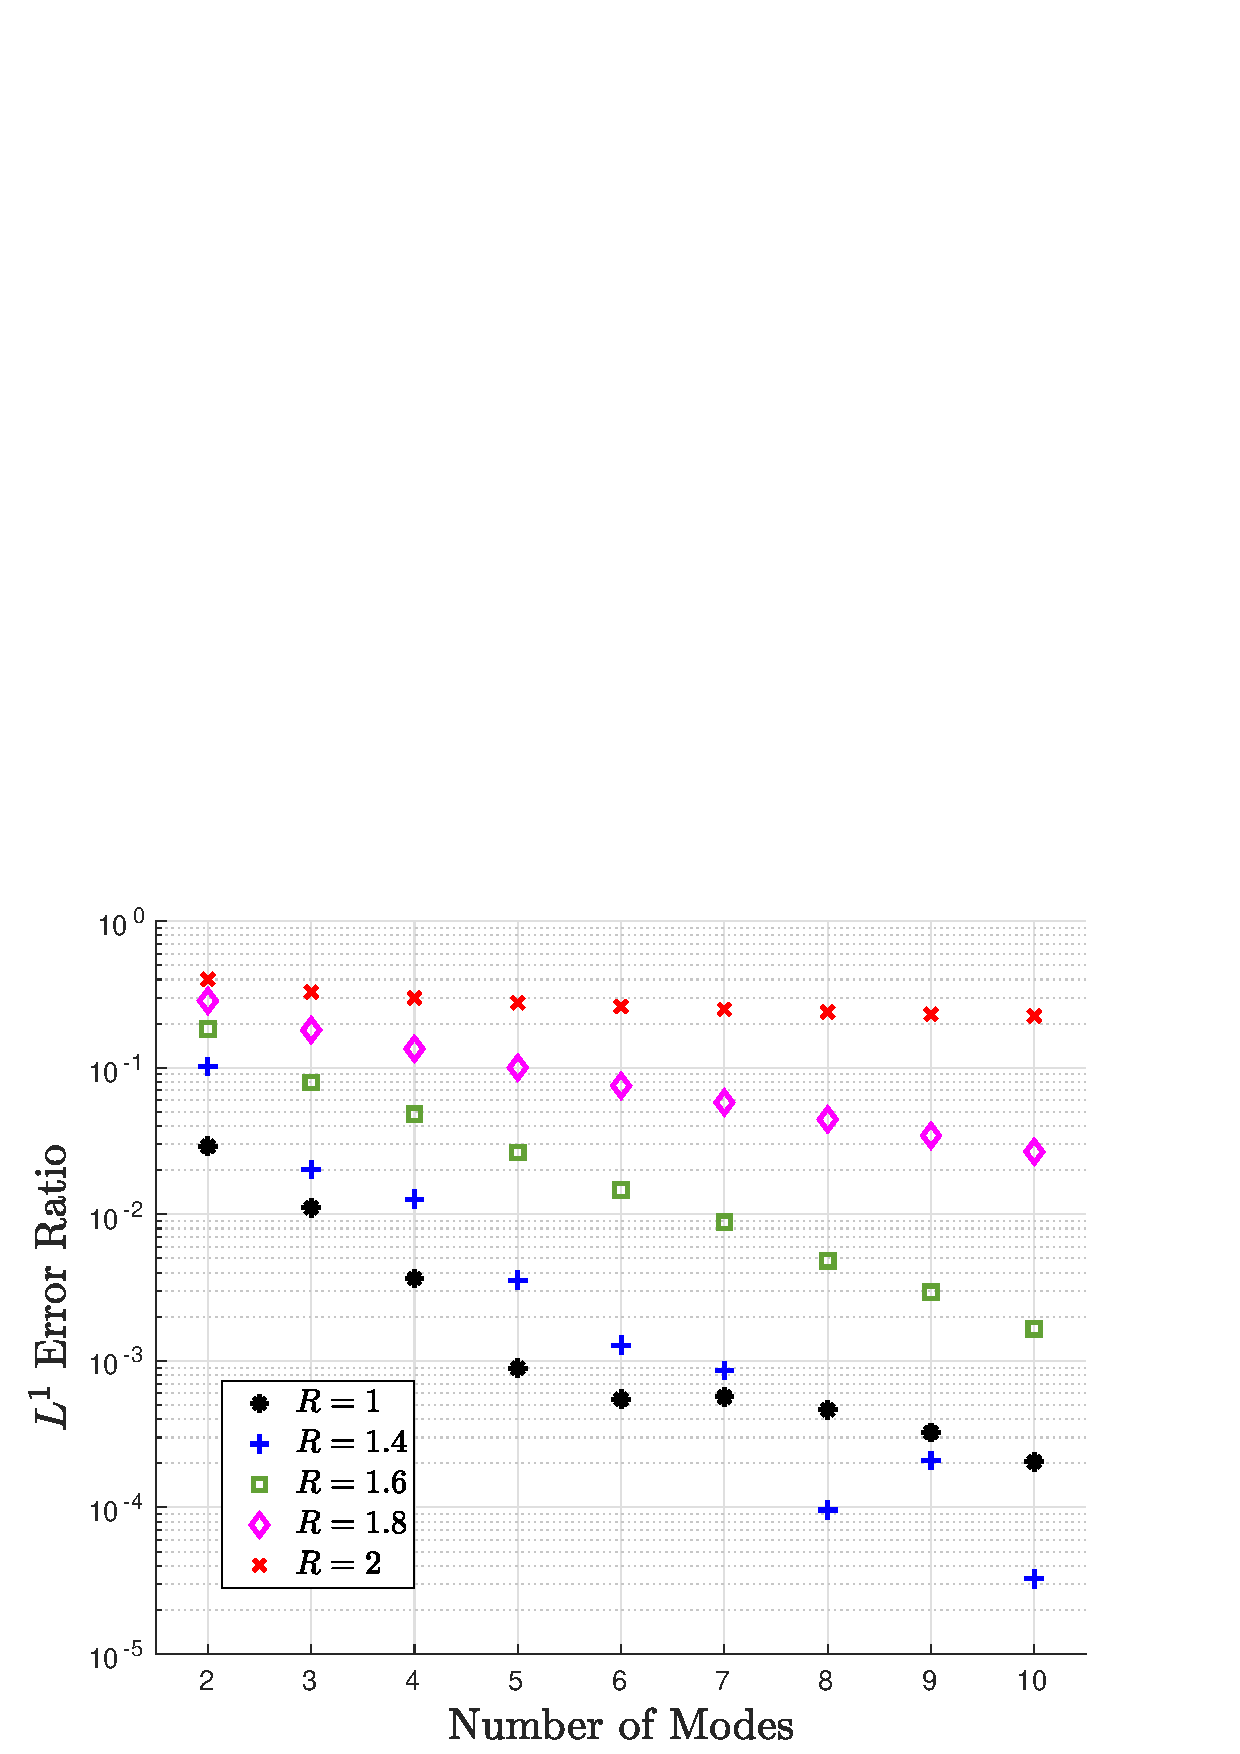
\includegraphics[width=0.8\linewidth]{06-appendix/SpectralMethodBoltzmann/Figures/free_stream_f0_approx_Ups_5.pdf}}
\caption{Errors in expansion of \req{zerothApprox} as a function of number of modes, $\Upsilon=0.5$. \radapt{Birrell:2014gea}.}\label{fig:freeStreamf0approxUps5}
 \centerline{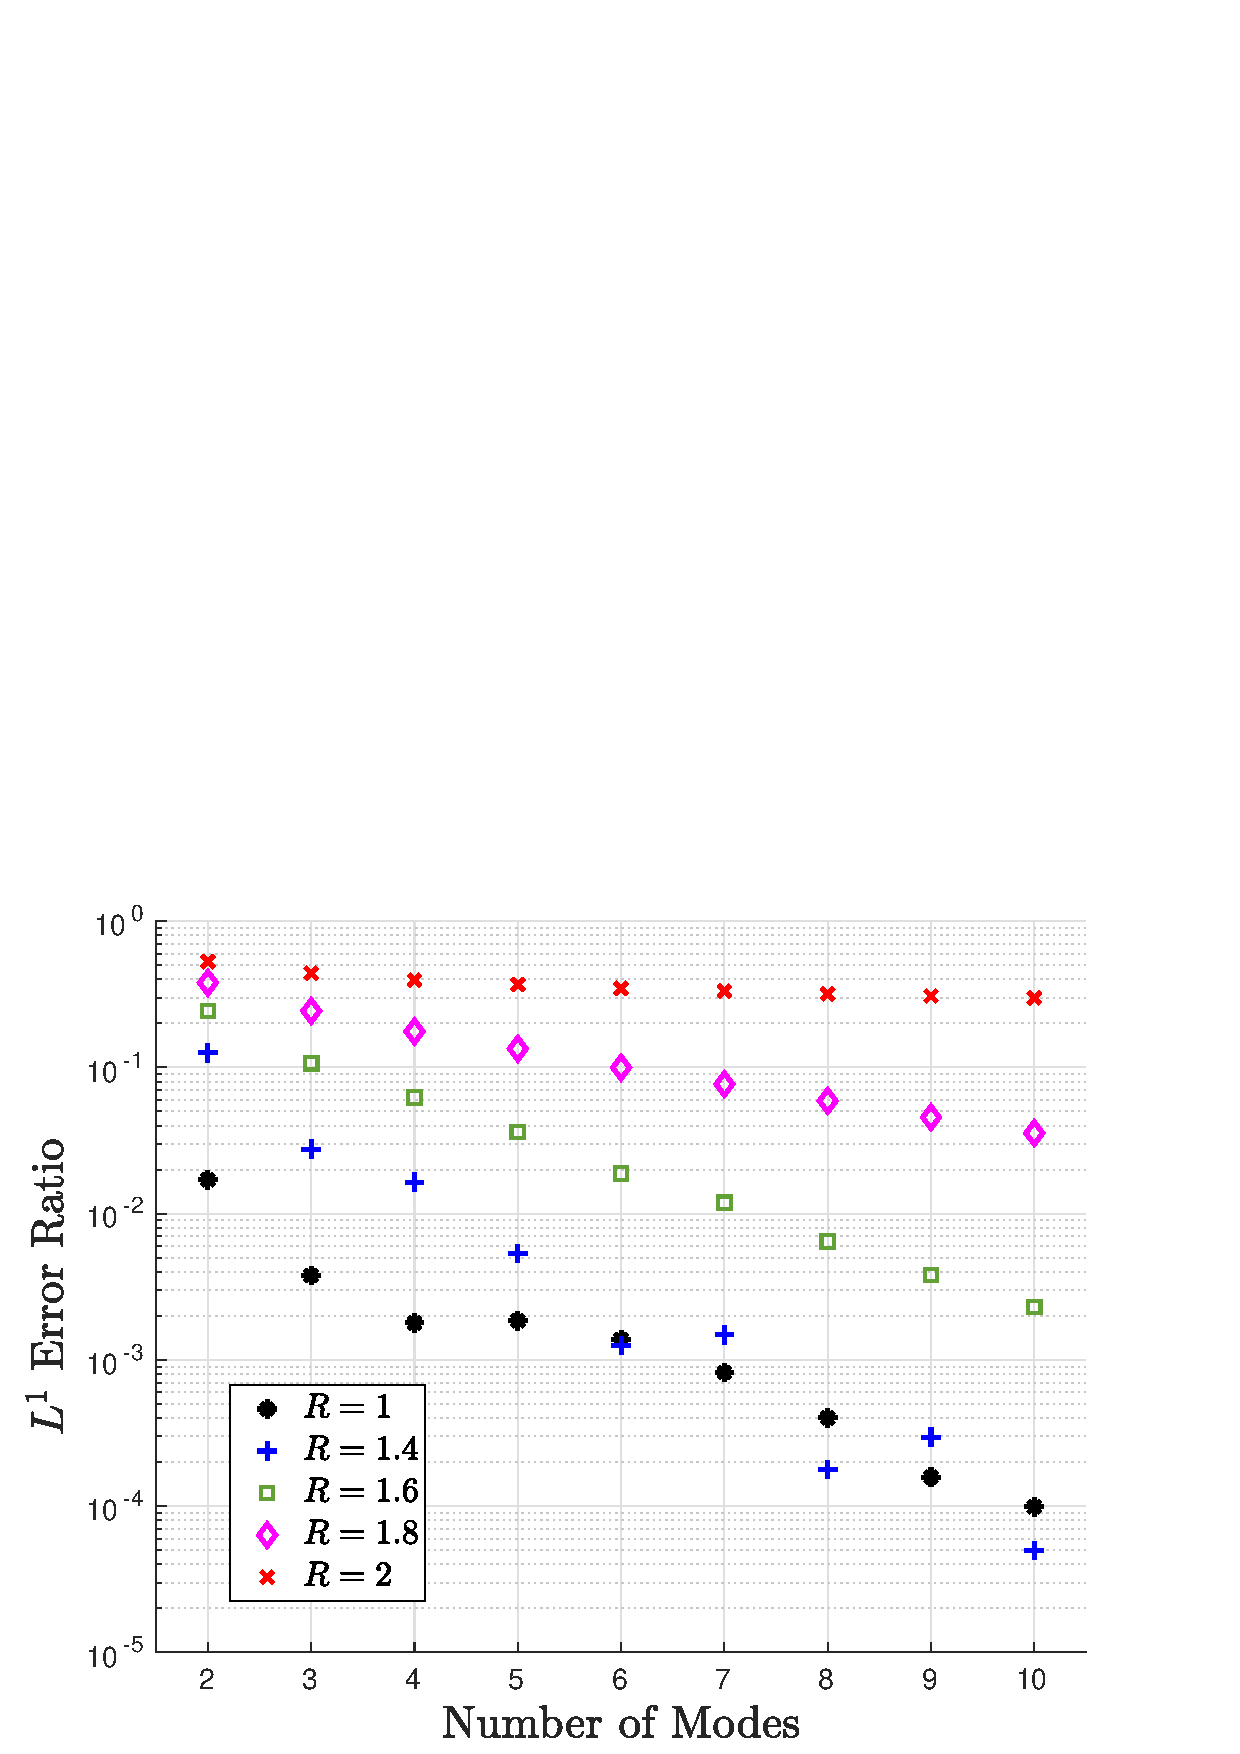
\includegraphics[width=0.8\linewidth]{06-appendix/SpectralMethodBoltzmann/Figures/free_stream_f0_approx_Ups_1_5.pdf}}
\caption{Errors in  expansion of \req{zerothApprox} as a function of number of modes, $\Upsilon=1.5$. \radapt{Birrell:2014gea}.}\label{fig:freeStreamf0approxUps15}
\end{figure}
%%%%%%%%%%%%%%%%%%%%%%%%%%%%%%%%%%%%


We note the appearance of the reheating ratio
\begin{equation}\label{reheat}
 R\equiv aT  
\end{equation}
in the denominator of \req{zerothApprox}, which comes from changing variables from $z=p/T$ in \req{weight} to $y=ap$ in order to compare with \req{freeStreamWeight}.  Physically, $R$ is the ratio of the physical temperature $T$ to the dilution controlled temperature scaling  of $1/a$.   In physical situations, including cosmology, $R$ can vary from unity when dimensioned energy scales influence dynamical equations for $a$. From the error plots we see that for $R$ sufficiently close to $1$, the approximation performs well with a small number of terms, even with $\Upsilon\neq 1$.  




 In the case of large reheating, we find that when $R$ approaches and surpasses $2$, large spurious oscillations begin to appear in the expansion and they persist even when a large number of terms are used, as seen in Figures  \ref{fig:freeStreamf0approxUps1Tr185} and \ref{fig:freeStreamf0approxUps1Tr2}, where we compare $f_\Upsilon/f_{ch}^{1/2}$ with $f_{\Upsilon}^N/f_{ch}^{1/2}$ for $\Upsilon=1$ and $N=20$. See Ref.~\cite{Birrell:2014gea} for further discussion of the origin of these oscillations. This demonstrates that the chemical equilibrium method with dilution temperature scaling will  perform extremely poorly in situations that experience a large degree of reheating. For $R\approx 1$, the benefit of including fugacity is not as striking, as the chemical equilibrium basis is able to approximate \req{zerothApprox} reasonably well.  However, for more stringent error tolerances including $\Upsilon$ can reduce the number of required modes in cases where the degree of chemical nonequilibrium is large.
%%%%%%%%%%%%%%%%%%%%%%%%%%%%%%%%%%%%%%%
\begin{figure}[ht]
\centerline{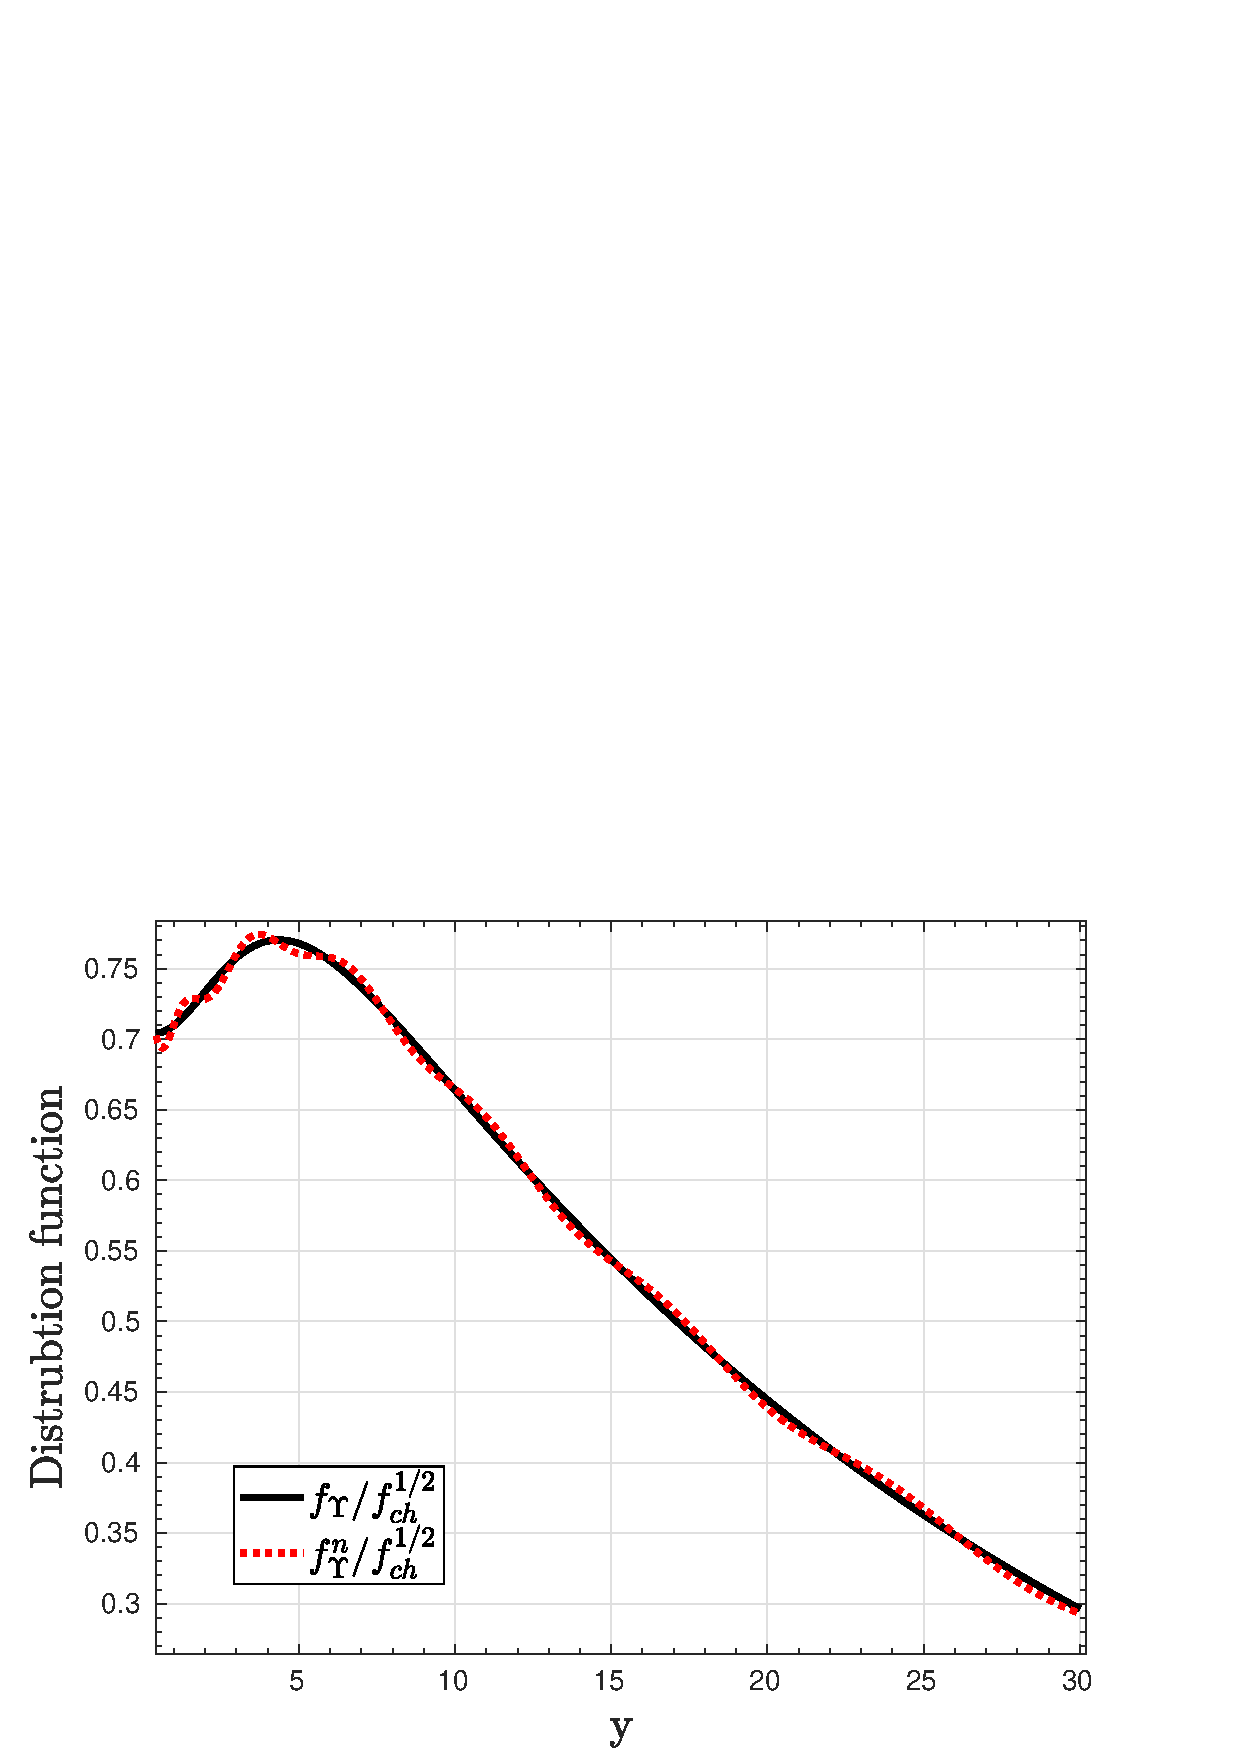
\includegraphics[width=0.8\linewidth]{06-appendix/SpectralMethodBoltzmann/Figures/free_stream_f0_approx_Ups_1_T_r_1_85_n_20.pdf}}
\caption{Approximation to \req{zerothApprox} for $\Upsilon=1$ and $R=1.85$ using the first $20$ basis elements generated by \req{freeStreamWeight}. \radapt{Birrell:2014gea}.}\label{fig:freeStreamf0approxUps1Tr185}
 \centerline{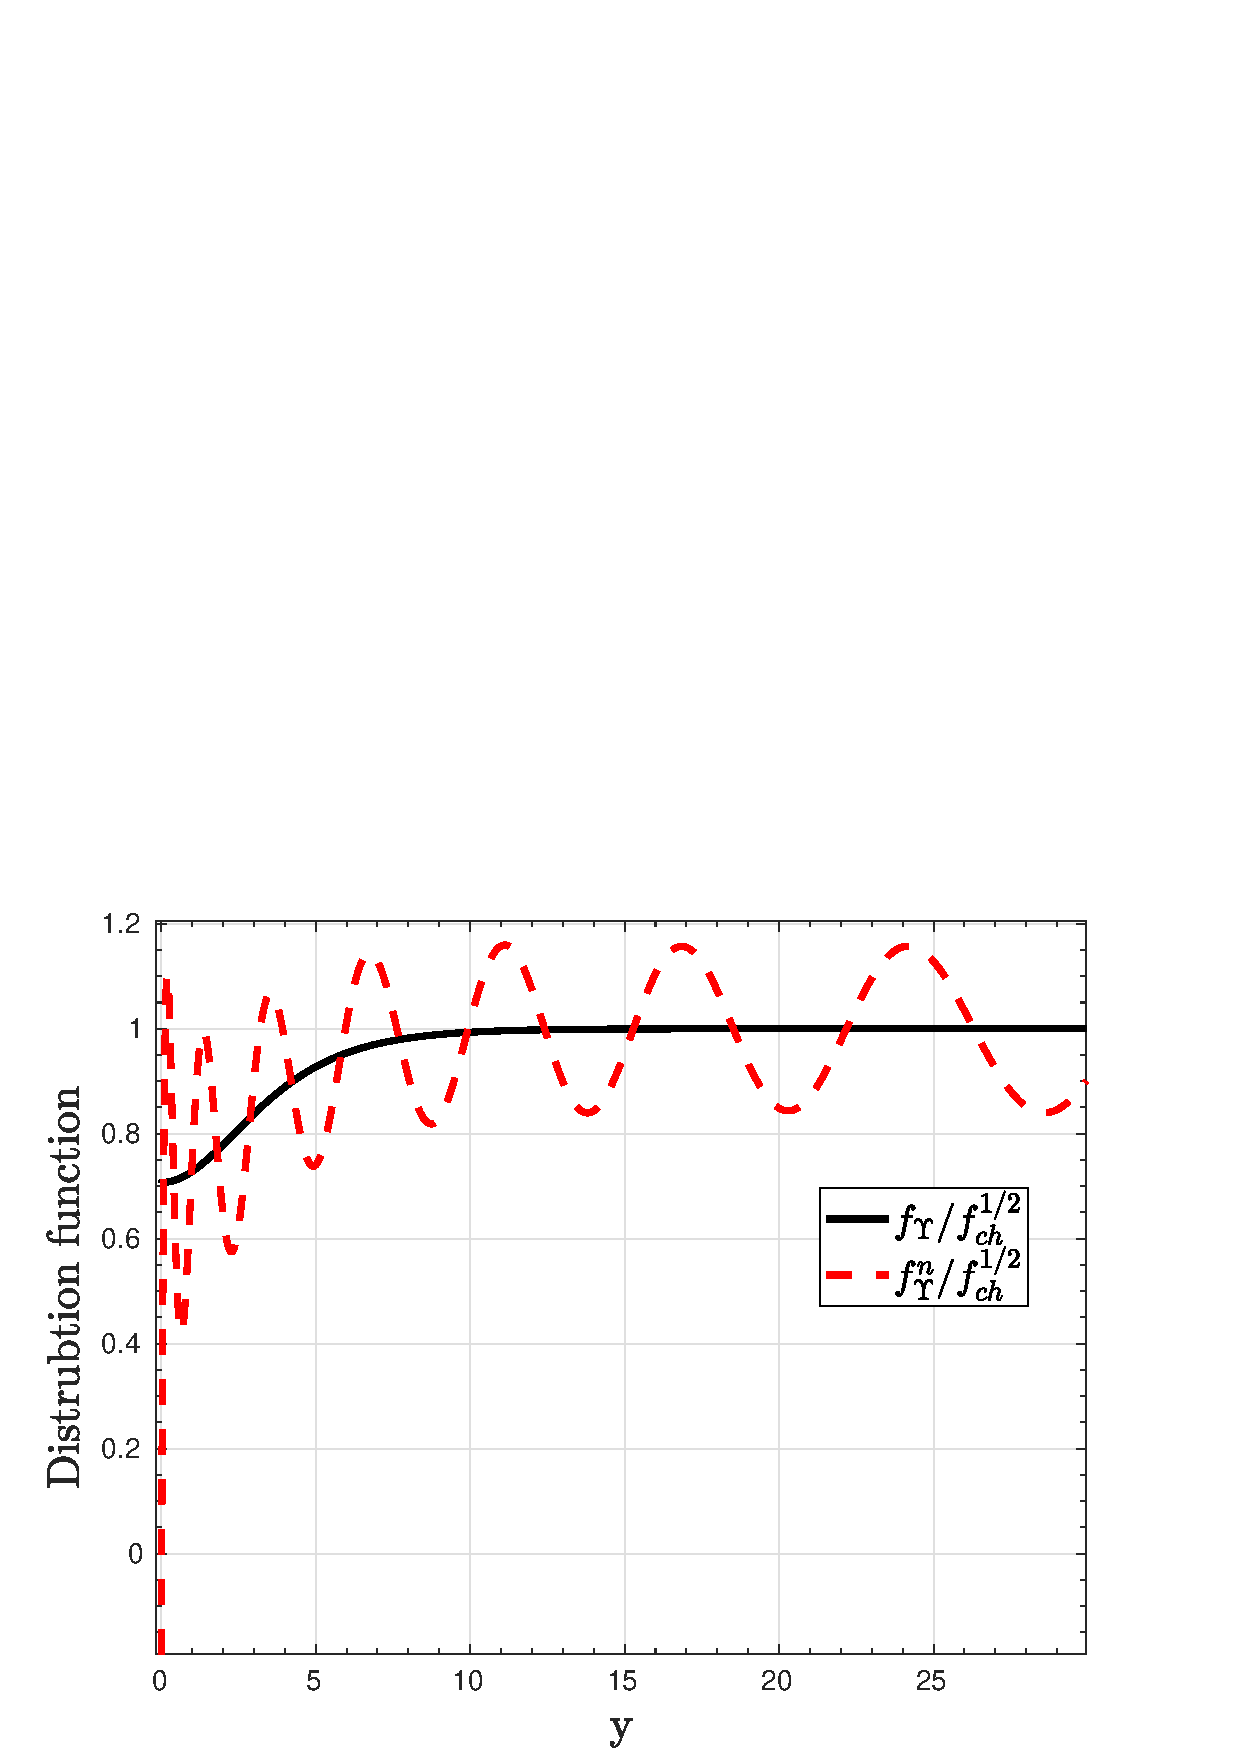
\includegraphics[width=0.8\linewidth]{06-appendix/SpectralMethodBoltzmann/Figures/free_stream_f0_approx_Ups_1_T_r_2_n_20.pdf}}
\caption{Approximation to \req{zerothApprox} for $\Upsilon=1$ and $R=2$ using the first $20$ basis elements generated by \req{freeStreamWeight}. \radapt{Birrell:2014gea}.}\label{fig:freeStreamf0approxUps1Tr2}
\end{figure}
%%%%%%%%%%%%%%%%%%%%%%%%%%%%%%%%%%%%

%%%%%%%%%%%%%%%%%%%%%%%%%%%%%%%%%%%%%%%%%%%%%%%%%%%%%%%%%%%
\para{Nonequilibrium dynamics}\label{dynamicsSec}
In this section we derive the dynamical equations for the chemical nonequilibrium method. In particular, we identify physically motivated dynamics for the effective temperature and fugacity. Using \req{TBoltzmann} and the definition of $\psi$ from \req{kineticApprox} we have
\begin{align}\label{nearEquilibEq}
\partial_t \psi+\frac{1}{f_\Upsilon }\frac{\partial f_\Upsilon }{\partial\Upsilon}\dot\Upsilon\psi-\frac{z}{f_\Upsilon }\left(H+\frac{\dot{T}}{T}\right)\left(\psi\partial_zf_\Upsilon +f_\Upsilon \partial_z \psi\right)=\frac{1}{f_\Upsilon E}C[f_\Upsilon \psi]\,.
\end{align}
Denote the monic orthogonal polynomial basis generated by the weight \req{weight} by $\psi_n$, $n=0,1,...$ where $\psi_n$ is degree $n$ and call the normalized versions  $\hat{\psi}_n$. Recall that $\hat\psi_n$ depend on $t$ due to the $\Upsilon$ dependence of the weight function used in the construction; therefore the method developed here is a moving-frame spectral method. Consider the space of polynomial of degree less than or equal to $N$, spanned by $\hat\psi_n$, $n=0,...,N$.   For $\psi$ in this subspace, we expand $\psi=\sum_{j=0}^Nb^j\hat\psi_j$ and use \req{nearEquilibEq}  to obtain
\begin{align}\label{Tvars}
\sum_i \dot{b}^i\hat\psi_i=&\sum_ib^i\frac{z}{f_\Upsilon }\left(H+\frac{\dot{T}}{T}\right)\left(\partial_z(f_\Upsilon )\hat\psi_i+f_\Upsilon \partial_z\hat\psi_i\right)\\
&-\sum_ib^i\left(\dot{\hat{\psi}}_i+\frac{1}{f_\Upsilon }\frac{\partial f_\Upsilon }{\partial\Upsilon}\dot\Upsilon\hat\psi_i\right)+\frac{1}{f_\Upsilon E}C[f]\,.
\notag
\end{align}
From this we see  that  projecting the Boltzmann-Einstein equation onto the finite dimensional subspace gives
\begin{align}
\dot b^k=& \sum_i b^i\left(H+\frac{\dot{T}}{T}\right)\left(\langle\frac{z}{f_\Upsilon }\hat\psi_i\partial_zf_\Upsilon ,\hat\psi_k\rangle+\langle z\partial_z \hat\psi_i,\hat\psi_k\rangle\right) \\
&-\sum_i b^i\dot{\Upsilon}\left(\langle\frac{1}{f_\Upsilon }\frac{\partial f_\Upsilon }{\partial\Upsilon}\hat\psi_i,\hat\psi_k\rangle+\langle\frac{\partial\hat{\psi}_i}{\partial \Upsilon},\hat\psi_k\rangle\right)+\langle\frac{1}{f_\Upsilon E}C[f],\hat\psi_k\rangle\notag\,,
\end{align}
where $\langle\cdot,\cdot\rangle$ denotes the inner product defined by the weight function \req{weight},
\begin{equation}
\langle h_1,h_2\rangle=\int_0^\infty h_1(z)h_2(z)w_\Upsilon(z)dz\,.
\end{equation}
The the collision term contains polynomial nonlinearities when multiple coupled distribution are being modeled using a $2$-$2$ collision operator \req{coll}, while the other terms are linear.  

To isolate the linear part, we define matrices
\begin{align}\label{ABmatrices}
A^k_i(\Upsilon)\equiv&\langle\frac{z}{f_\Upsilon }\hat\psi_i\partial_zf_\Upsilon ,\hat\psi_k\rangle+\langle z\partial_z \hat\psi_i,\hat\psi_k\rangle\,,\\
B^k_i(\Upsilon)\equiv& C_i^k(\Upsilon)+D_i^k(\Upsilon),\hspace{2mm} C_i^k\equiv\Upsilon\langle\frac{1}{f_\Upsilon }\frac{\partial f_\Upsilon }{\partial\Upsilon}\hat\psi_i,\hat\psi_k\rangle,\hspace{2mm} D_i^k\equiv\Upsilon\langle\frac{\partial\hat{\psi}_i}{\partial \Upsilon},\hat\psi_k\rangle\,. \notag
\end{align}
 With these definitions, the equations for the $b^k$ become
\begin{align}\label{bEq}
\dot b^k=& \left(H+\frac{\dot{T}}{T}\right)\sum_i A_i^k(\Upsilon)b^i-\frac{\dot{\Upsilon}}{\Upsilon}\sum_i B_i^k(\Upsilon)b^i+\langle\frac{1}{f_\Upsilon E}C[f],\hat\psi_k\rangle\,.
\end{align}
 See Section \ref{sec:orthopolyApp} for details on how to recursively construct the $\partial_z\hat\psi_i$. We showed how to compute the inner products $\langle\hat\psi_k,\partial_{\Upsilon}\hat\psi_k\rangle$ in  Section \ref{ortho-polynom-fam}. In  \req{eq:lowerTri1}-\req{eq:lowerTri5} we proved that that both $A$ and $B$ are lower triangular and show that the only inner products involving the $\partial_\Upsilon\hat{\psi}_i$ that are required in order to compute $A$ and $B$ are those the above mentioned diagonal elements, $\langle\hat\psi_k,\partial_{\Upsilon}\hat\psi_k\rangle$.


We fix the dynamics of $T$ and $\Upsilon$ by imposing the conditions
\begin{equation}\label{bIcs}
b^0(t)\hat\psi_0(t)=1\,,\hspace{2mm}b^1(t)=0\,.
\end{equation}
In other words,
\begin{equation}
f(t,z)=f_\Upsilon (t,z)\left(1+\phi(t,z)\right),\hspace{2mm} \phi=\sum_{i=2}^N b^i\hat\psi_i\,.
\end{equation}
This reduces the number of degrees of freedom in \req{bEq} from $N+3$ to $N+1$.  In other words, after enforcing \req{bIcs}, \req{bEq} constitutes $N+1$ equations for the remaining $N+1$ unknowns, $b^2,...,b^N$, $\Upsilon$, and $T$.  We will call $T$ and $\Upsilon$ the first two ``modes", as their dynamics arise from imposing the conditions \req{bIcs} on the zeroth and first order coefficients in the expansion. We will solve for their dynamics explicitly below.

To see the physical motivation for the choices \req{bIcs}, consider the particle number density and energy density.  Using orthonormality of the $\hat\psi_i$ and \req{bIcs} we have
\begin{align}
n=&\frac{g_pT^3}{2\pi^2}\sum_ib^i\int_0^\infty f_\Upsilon  \hat\psi_i z^2 dz=\frac{g_pT^3}{2\pi^2}\sum_ib^i\langle \hat\psi_i ,1\rangle\\
=&\frac{g_pT^3}{2\pi^2}b^0\langle \hat\psi_0 ,1\rangle=\frac{g_pT^3}{2\pi^2}\langle 1 ,1\rangle\,,\notag\\
\rho=&\frac{g_pT^4}{2\pi^2}\sum_ib^i\int_0^\infty f_\Upsilon  \hat\psi_i z^3 dz=\frac{g_pT^4}{2\pi^2}\sum_ib^i\langle\hat\psi_i, z\rangle\\
=&\frac{g_pT^4}{2\pi^2}\left(b^0\langle\hat\psi_0, z\rangle+b^1\langle\hat\psi_1, z\rangle\right)=
\frac{g_pT^4}{2\pi^2}\langle 1,z\rangle\,.\notag
\end{align}
These, together with the definition of the weight function \req{weight}, imply
\begin{align}\label{thEqMoments}
n=&\frac{g_pT^3}{2\pi^2}\int_0^\infty f_\Upsilon  z^2dz\,,\\
\label{thEqMoments2}
\rho=&\frac{g_pT^4}{2\pi^2}\int_0^\infty f_\Upsilon  z^3dz\,.
\end{align}
Equations (\ref{thEqMoments}) and (\ref{thEqMoments2}) show  that the first two modes, $T$ and $\Upsilon$, with time evolution fixed by \req{bIcs} cause the chemical nonequilibrium distribution $f_\Upsilon $ to capture the number density and energy density of the system exactly.  This fact is very significant, as it implies that within the chemical nonequilibrium approach as long as the back-reaction from the non-thermal distortions is small (meaning that the evolution of $T(t)$ and $\Upsilon(t)$ is not changed significantly when more modes are included), {\em all the effects relevant to the computation of  particle and energy flow are modeled by the time evolution of $T$ and $\Upsilon$ alone} and no further modes are necessary.  This gives a clear separation between the averaged physical quantities, characterized by $f_\Upsilon $, and the momentum dependent non-thermal distortions as captured by 
\begin{equation}
\phi=\sum_{i=2}^N b^i\hat\psi_i\,.
\end{equation}

One should contrast this chemical nonequilibrium behavior  with the chemical equilibrium method, where a minimum of four modes is required to describe the number and energy densities, as shown in \req{freeStreamMoments}.   Moreover we will show that convergence to the desired precision is faster in the chemical nonequilibrium approach as compared to chemical equilibrium. Due to the high cost of numerically integrating realistic collision integrals of the form \req{coll}, this fact can be very significant in applications. We remark that the relations \req{thEqMoments} are the physical motivation for including the $z^2$ factor in the weight function. All three modifications we have made in constructing our new method, the introduction of an effective temperature, i.e., $R\ne 1$, the generalization to chemical nonequilibrium $f_\Upsilon $, and the introduction of $z^2$ to the weight, \req{reheat}, were needed to obtain the properties \req{thEqMoments}, but it is the introduction of $z^2$ that reduces the number of required modes and hence reduces the computational cost. 

With $b^0$ and $b^1$ fixed as in \req{bIcs} we can solve the equations for $\dot b^0$ and $\dot b^1$ from \req{bEq} for $\dot\Upsilon$ and $\dot T$ to obtain

\begin{align}\label{UpsTEqs}
\dot{\Upsilon}/{\Upsilon}=&\frac{(Ab)^1\langle\frac{1}{f_\Upsilon E}C[f],\hat\psi_0\rangle-(Ab)^0\langle\frac{1}{f_\Upsilon E}C[f],\hat\psi_1\rangle }{[\Upsilon\partial_\Upsilon \langle1,1\rangle/(2||\psi_0||)+(Bb)^0](Ab)^1-(Ab)^0(Bb)^1}\,,\\[0.5cm]
\dot{T}/T
=&\frac{(Bb)^1\langle\frac{1}{f_\Upsilon E}C[f],\hat\psi_0\rangle-\langle\frac{1}{f_\Upsilon E}C[f],\hat\psi_1\rangle[\Upsilon\partial_\Upsilon \langle1,1\rangle/(2||\psi_0||)+(Bb)^0]}{[\Upsilon\partial_\Upsilon \langle1,1\rangle/(2||\psi_0||)+(Bb)^0](Ab)^1-(Ab)^0(Bb)^1}-H\notag\\[0.3cm]
=&\frac{1}{(Ab)^1}\left((Bb)^1\dot{\Upsilon}/\Upsilon-\langle\frac{1}{f_\Upsilon E}C[f],\hat\psi_1\rangle\right)-H\,.\label{Teq}
\end{align}

Here $(Ab)^n=\sum_{j=0}^NA^n_jb^j$ and similarly for $B$ and $||\cdot||$ is the norm induced by $\langle\cdot,\cdot\rangle$. In deriving this, we used
\begin{equation}
\dot{b}^0=\frac{1}{2||\psi_0||}\dot\Upsilon\partial_\Upsilon \langle1,1\rangle\,, \hspace{4mm} \partial_\Upsilon \langle1,1\rangle=\int_0^\infty \frac{z^2}{(e^{z/2}+ \Upsilon e^{-z/2})^2}dz\,,
\end{equation}
which comes from differentiating \req{bIcs}. 
 
It is easy to check that when the collision operator vanishes, then the above system is solved by 
\begin{equation}\label{freeStreamSol}
\Upsilon=\text{constant}\,,\hspace{4mm} \frac{\dot T}{T}=-H\,,\hspace{2mm}  b^n=\text{constant}\,,\hspace{1mm} n>2\,,
\end{equation}
i.e., the fugacity and non-thermal distortions are `frozen' into the distribution and the temperature satisfies dilution scaling $T\propto 1/a$.

When the collision term becomes small, \req{freeStreamSol} motivates another change of variables. Letting $T=(1+\epsilon)/a$  gives the equation
\begin{equation}
\dot\epsilon=\frac{1+\epsilon}{(Ab)^1}\left((Bb)^1\dot{\Upsilon}/\Upsilon-\langle\frac{1}{f_\Upsilon E}C[f],\hat\psi_1\rangle\right).
\end{equation}
Solving this in place of \req{Teq} when the collision terms are small avoids having to numerically track the free-streaming evolution. In particular this will ensure conservation of comoving particle number, which equals a function of $\Upsilon$ multiplied by $(aT)^3$, to much greater precision in this regime as well as resolve the freeze-out temperatures more accurately.\\

%%%%%%%%%%%%%%%%%%%%%%%%%%%%%%%%%%%%%%%%%%%%%%%%%%%%%%%%%%
\noindent{\bf Projected Dynamics are Well-defined:}\\
The following calculation shows that, for a distribution initially in kinetic equilibrium, the determinant factor in the denominator of \req{UpsTEqs} is nonzero and hence the dynamics for $T$ and $\Upsilon$, as well as the remainder of the projected system, are well-defined, at least for sufficiently small times. 

Kinetic equilibrium\index{kinetic equilibrium} implies the initial conditions $b^0=||\psi_0||$, $b^i=0$, $i>0$.  Therefore we have
\begin{align}
K\equiv& (\Upsilon\partial_\Upsilon \langle 1,1\rangle/(2||\psi_0||)+(Bb)^0)(Ab)^1-(Ab)^0(Bb)^1\\[0.3cm]
=&(C^0_0A^1_0-A^0_0C^1_0)(b^0)^2+\left[(D^0_0A^1_0-A^0_0D^1_0)(b^0)^2+\Upsilon\partial_\Upsilon \langle 1,1\rangle/(2||\psi_0||)A^1_0b^0\right]\notag\\[0.3cm]
\equiv & K_1+K_2\,.\notag
\end{align}
\begin{align}
K_1=&\langle \frac{1}{1+\Upsilon e^{-z}},1\rangle\langle \frac{-z}{1+\Upsilon e^{-z}}\hat\psi_1,\hat\psi_0\rangle-\langle\frac{-z}{1+\Upsilon e^{-z}},\hat\psi_0\rangle\langle\frac{1}{1+ \Upsilon e^{-z}}\hat\psi_1,1\rangle\,.
\end{align}
Inserting the formula for $\hat\psi_1$ from \req{polyRecursion} we find
\begin{align}
K_1=&-\frac{1}{||\psi_1||\,||\psi_0||}\left[\langle\frac{1}{1+ \Upsilon e^{-z}},\hat\psi_0\rangle\langle\frac{z^2}{1+\Upsilon e^{-z}},\hat\psi_0\rangle-\langle\frac{z}{1+\Upsilon e^{-z}},\hat\psi_0\rangle^2\right]\,.
\end{align}
The Cauchy-Schwarz inequality  applied to the inner product with weight function
\begin{equation}
\tilde{w}=\frac{w}{1+\Upsilon e^{-z}}\hat\psi_0
\end{equation}
together with linear independence of $1$ and $z$ implies that the term in brackets is positive and so $K_1<0$ at $t=0$.  For the second term, noting that $D^1_0=0$ by orthogonality and using \req{normDerivEq}, we have
\begin{align}
K_2=&[\langle\partial_\Upsilon\hat\psi_0,\hat\psi_0\rangle||\psi_0||+\partial_\Upsilon \langle 1,1\rangle/(2||\psi_0||)]\Upsilon A_0^1||\psi_0||=0\,.
\end{align}
This proves that $K$ is nonzero at $t=0$.\\

%%%%%%%%%%%%%%%%%%%%%%%%%%%%%%%%%%%%%%%%%%%%%
\subsection{Validation}\label{validation}
We will validate our numerical method on an exactly solvable model problem
\begin{equation}\label{toyEq}
\partial_t f-pH \partial_p f=M\left(\frac{1}{\Upsilon^{-1}e^{p/T_{eq}}+1}-f(p,t)\right)\,, \hspace{2mm} f(p,0)=\frac{1}{e^{p/T_{eq}(0)}+1}\,,
\end{equation}
where $M$ is a constant with units of energy and we choose units in which it is equal to $1$. This model describes a distribution that is attracted to a given equilibrium distribution at a prescribed time dependent temperature $T_{eq}(t)$ and fugacity\index{fugacity} $\Upsilon$. This type of an idealized scattering operator, without fugacity, was first introduced in \cite{Anderson:1974nyl}. By changing coordinates $y=a(t)p$ we find
\begin{equation}\label{freeStreamToy}
\partial_tf(y,t)=\frac{1}{\Upsilon^{-1}\exp[y/(a(t)T_{eq}(t))]+1}-f(y,t)\,.
\end{equation}
 which has as solution
\begin{equation}\label{exactSol}
f(y,t)=\int_0^t\frac{e^{s-t}}{\Upsilon^{-1}\exp[y/(a(s)T_{eq}(s))]+1}ds+\frac{e^{-t}}{\exp[y/(a(0)T_{eq}(0))]+1}\,.
\end{equation}
We now transform to $z=p/T(t)$ where the temperature $T$ of the distribution $f$ is defined as in Section \ref{dynamicsSec}.  Therefore, we have the exact solution to
\begin{equation}\label{kEqToy}
\partial_tf-z\left(H+\frac{\dot{T}}{T}\right)\partial_zf=\frac{1}{\Upsilon^{-1}e^{zT/T_{eq}}+1}-f(z,t)
\end{equation}
given by
\begin{align}
f(z,t)=&\int_0^t\frac{e^{s-t}}{\Upsilon^{-1}\exp[a(t)T(t)z/(a(s)T_{eq}(s))]+1}ds\\
&+\frac{e^{-t}}{\exp[a(t)T(t)z/(a(0)T_{eq}(0))]+1}\,.\notag
\end{align}
We use this to test the chemical equilibrium and chemical nonequilibrium methods under two different conditions. 

%%%%%%%%%%%%%%%%%%%%%%%%%%%%%%%%%%%%%%%%%%%%%%%%%%%%%%%%%%%%%%%%%%%%%
\para{Reheating Test}
First we compare the chemical equilibrium\index{chemical equilibrium} and nonequilibrium methods in a scenario that exhibits reheating.  Motivated by applications to cosmology, we choose a scale factor evolving as in the radiation dominated era, a fugacity $\Upsilon=1$, and choose an equilibrium temperature that exhibits reheating like behavior with $aT_{eq}$ increasing for a period of time,
\begin{align}\label{aTDef}
a(t)=\left(\frac{t+b}{b}\right)^{1/2}\,,\ \  \ \
T_{eq}(t)=\frac{1}{a(t)}\left(1+\frac{1-e^{-t}}{e^{-(t-b)}+1}(R-1)\right)\,,
\end{align}
where $R$ is the desired reheating ratio. Note that $(aT_{eq})(0)=1$ and $(aT_{eq})(t)\rightarrow R$ as $t\rightarrow\infty$. Qualitatively, this is reminiscent of the dynamics of neutrino freeze-out, but the range of reheating ratio for which we will test our method is larger than found there.

We solved \req{freeStreamToy} and \req{kEqToy} numerically using the chemical equilibrium and chemical nonequilibrium methods respectively for $t\in[0,10]$ and $b=5$ and the cases $R=1.1$, $R=1.4$, as well as the more extreme ratio of $R=2$.  The bases of orthogonal polynomials were generated numerically using the recursion relations from \ref{sec:orthopolyApp}.  For the applications we are considering, where the solution is a small perturbation of equilibrium, only a small number of terms are required and so the numerical challenges associated with generating a large number of such orthogonal polynomials are not an issue.\\

%%%%%%%%%%%%%%%%%%%%%%%%%%%%%%%%%%%%%%%%%%%%%
\noindent{\bf Chemical Equilibrium Method:}\\
We solved \req{freeStreamToy} using the chemical equilibrium method, with the orthonormal basis defined by the weight function \req{freeStreamWeight} for $N=2,...,10$ modes (mode numbers $n=0,...,N-1$) and prescribed  single step relative and absolute error tolerances of $10^{-13}$ for the numerical integration, and with asymptotic reheating ratios of $R=1.1$, $R=1.4$, and $R=2$.   



In Figures \ref{fig:freeStreamNumErr} and  \ref{fig:freeStreamEerr} we show the maximum relative error in the number densities and energy densities respectively over the time interval $[0,10]$ for various numbers of computed modes.  The particle number density and energy density are accurate, up to the integration tolerance level, for $3$ or more and $4$ or more modes respectively. This is consistent with \req{freeStreamMoments} which shows the number of modes required to capture each of these quantities. However, fewer modes than these minimum values lead to a large error in the corresponding moment of the distribution function.
%%%%%%%%%%%%%%%%%%%%%%%%%%%%%%%%%%%%%%%
\begin{figure}
\centerline{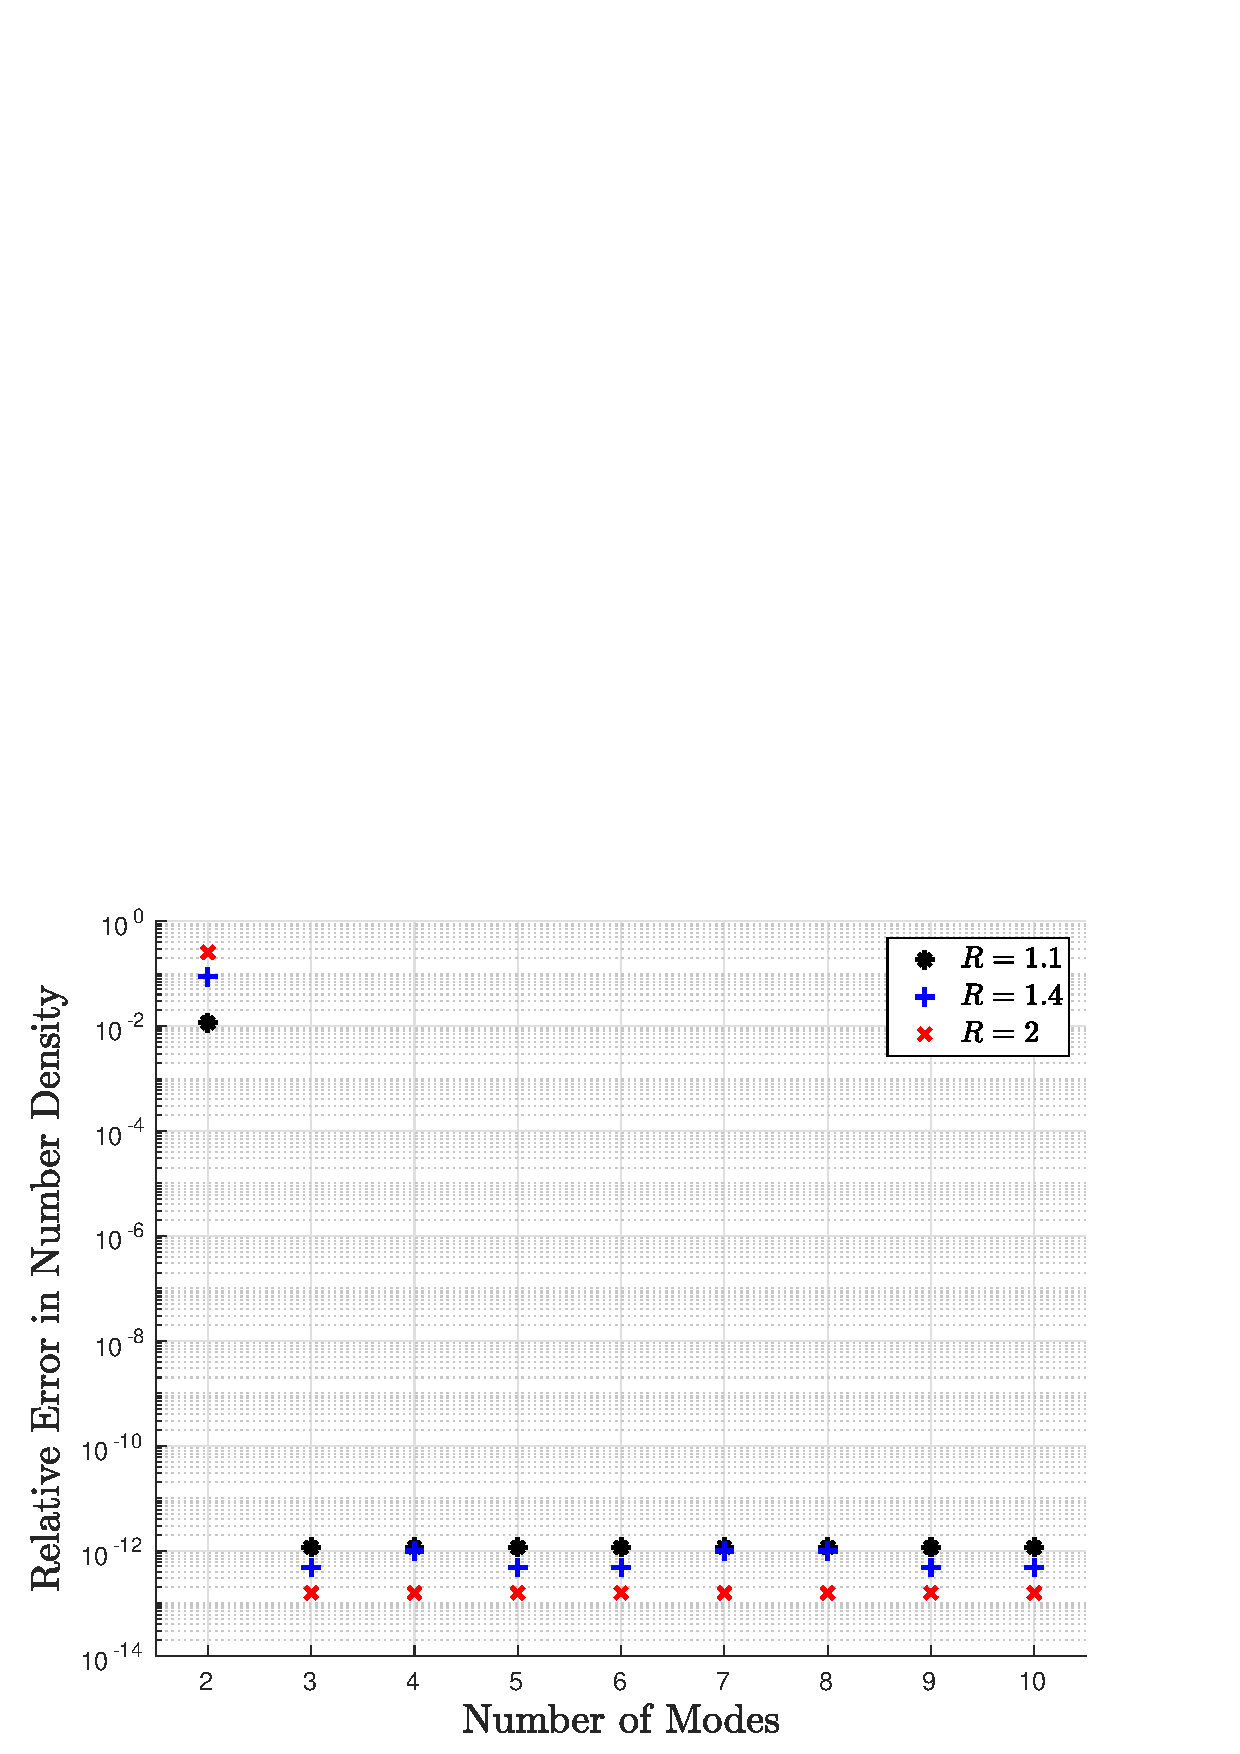
\includegraphics[width=0.8\linewidth]{06-appendix/SpectralMethodBoltzmann/Figures/free_stream_num_err.pdf}}
\caption{Maximum relative error in particle number density. \radapt{Birrell:2014gea}.}\label{fig:freeStreamNumErr}
\centerline{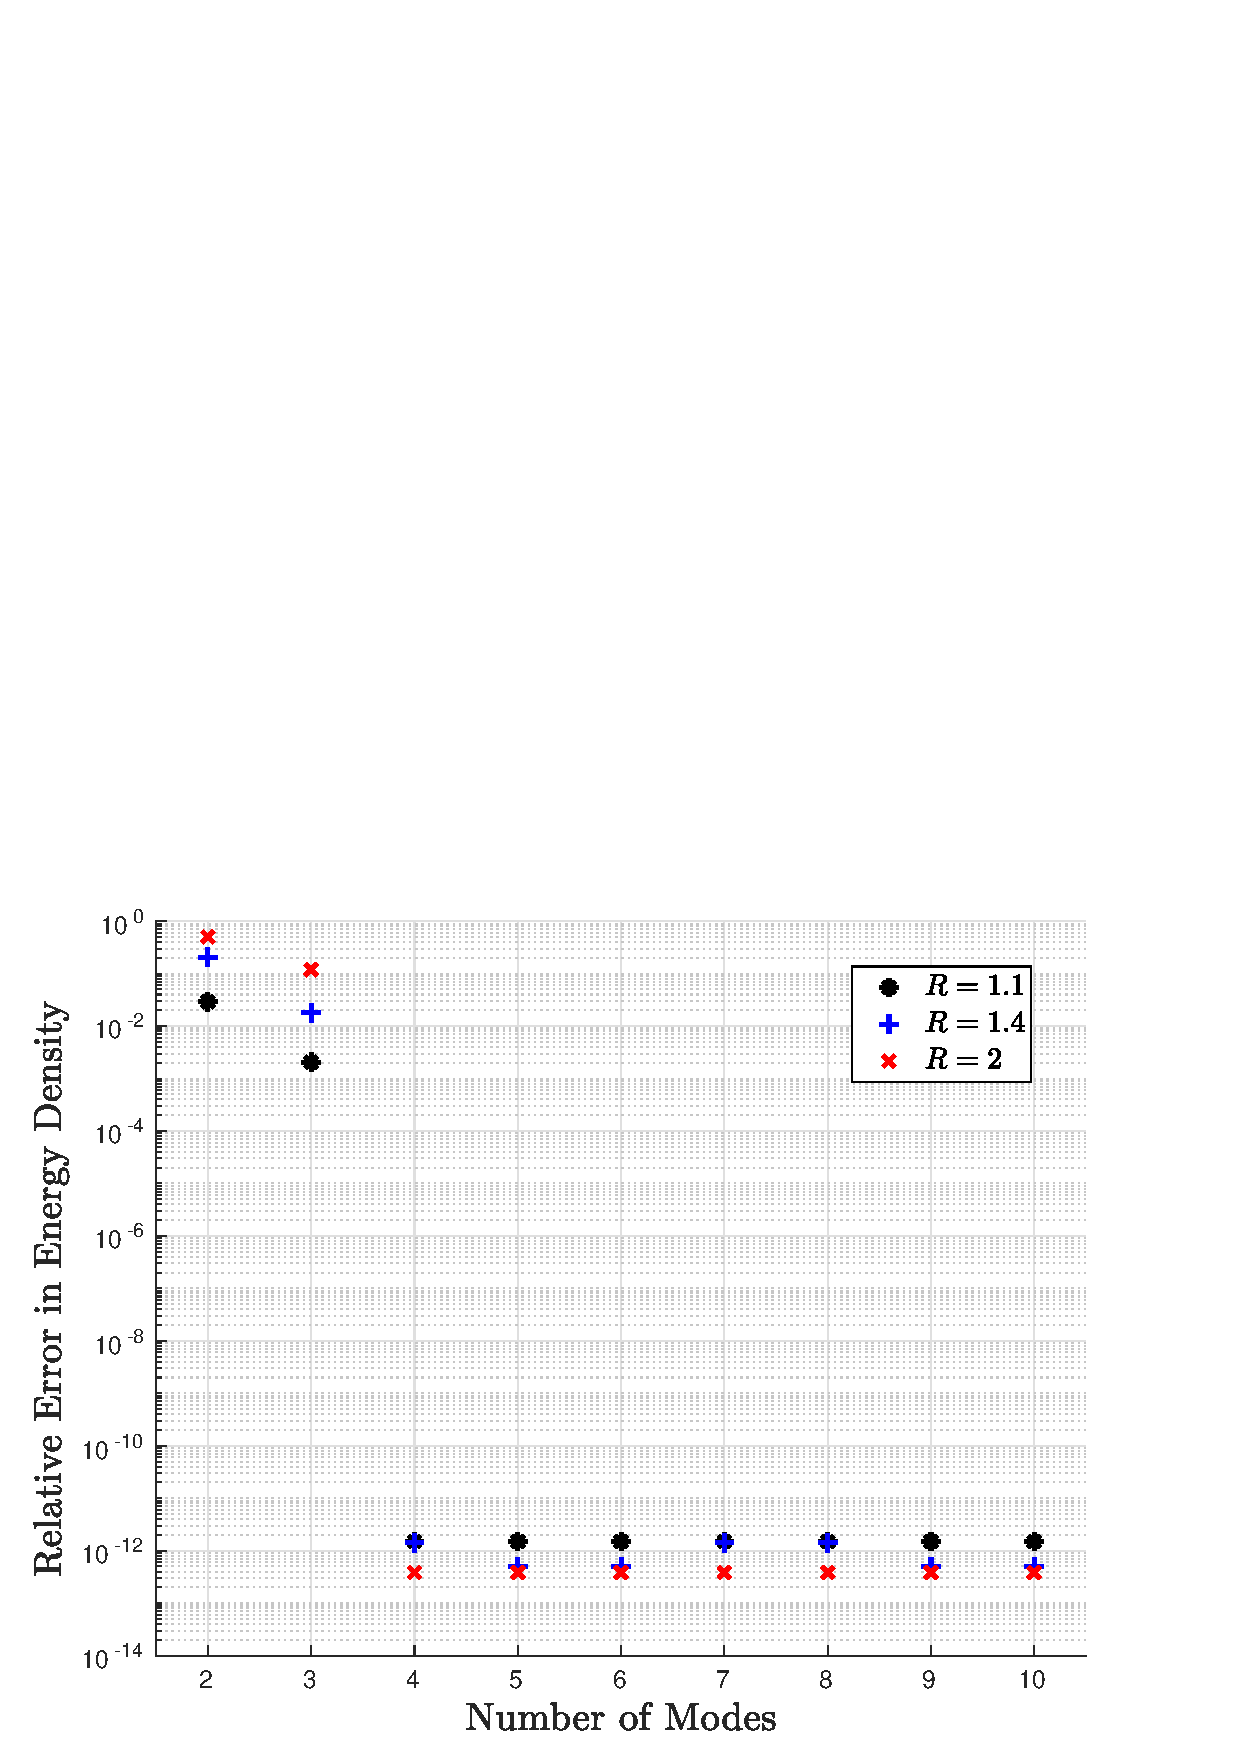
\includegraphics[width=0.8\linewidth]{06-appendix/SpectralMethodBoltzmann/Figures/free_stream_E_err.pdf}}
\caption{Maximum relative error in energy density. \radapt{Birrell:2014gea}.}\label{fig:freeStreamEerr}
\end{figure}
%%%%%%%%%%%%%%%%%%%%%%%%%%%%%%%%%%%%%%%

%%%%%%%%%%%%%%%%%%%%%%%%%%%%%%%%%%%%%%%
\begin{figure}[ht]
\centerline{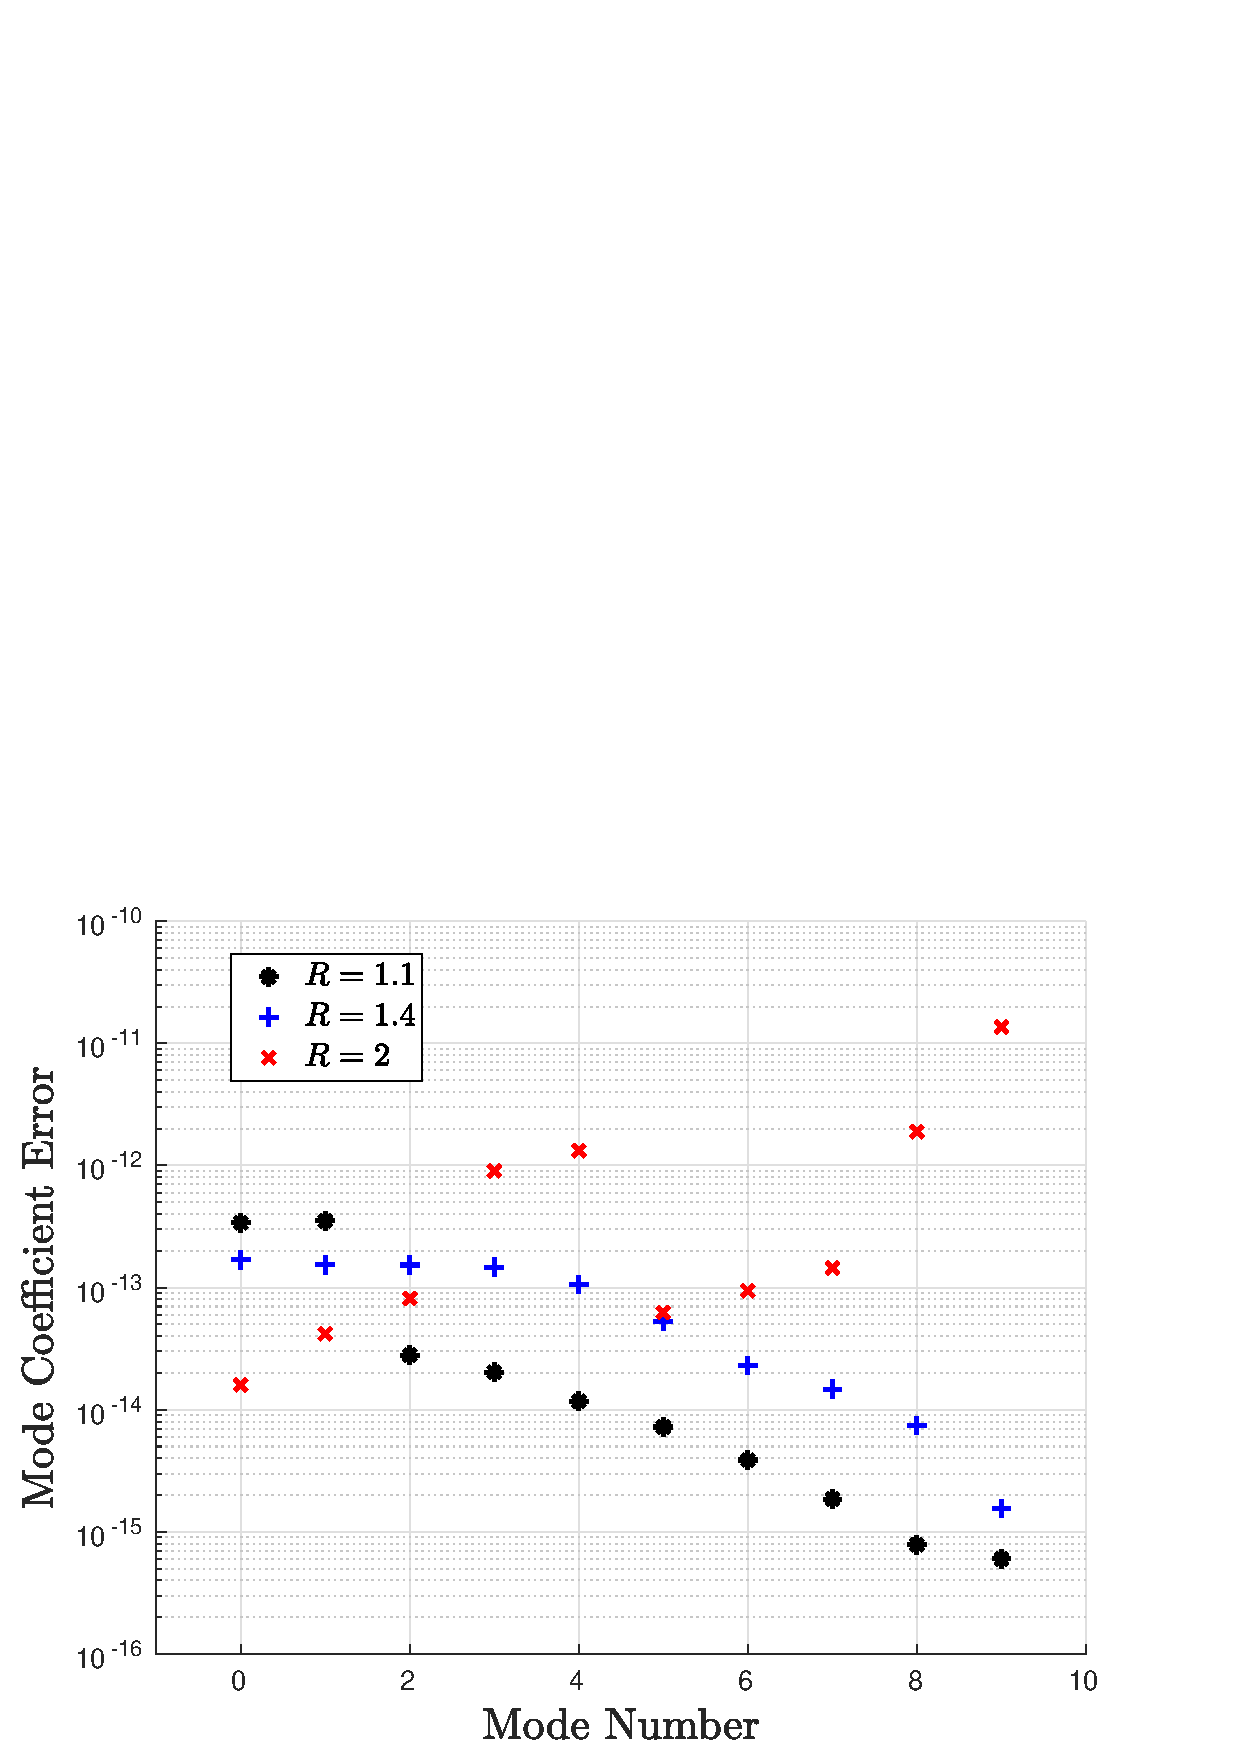
\includegraphics[width=0.8\linewidth]{06-appendix/SpectralMethodBoltzmann/Figures/free_stream_b_err.pdf}}
\caption{Maximum error in mode coefficients. \radapt{Birrell:2014gea}.}\label{fig:freeStreambErr}
\centerline{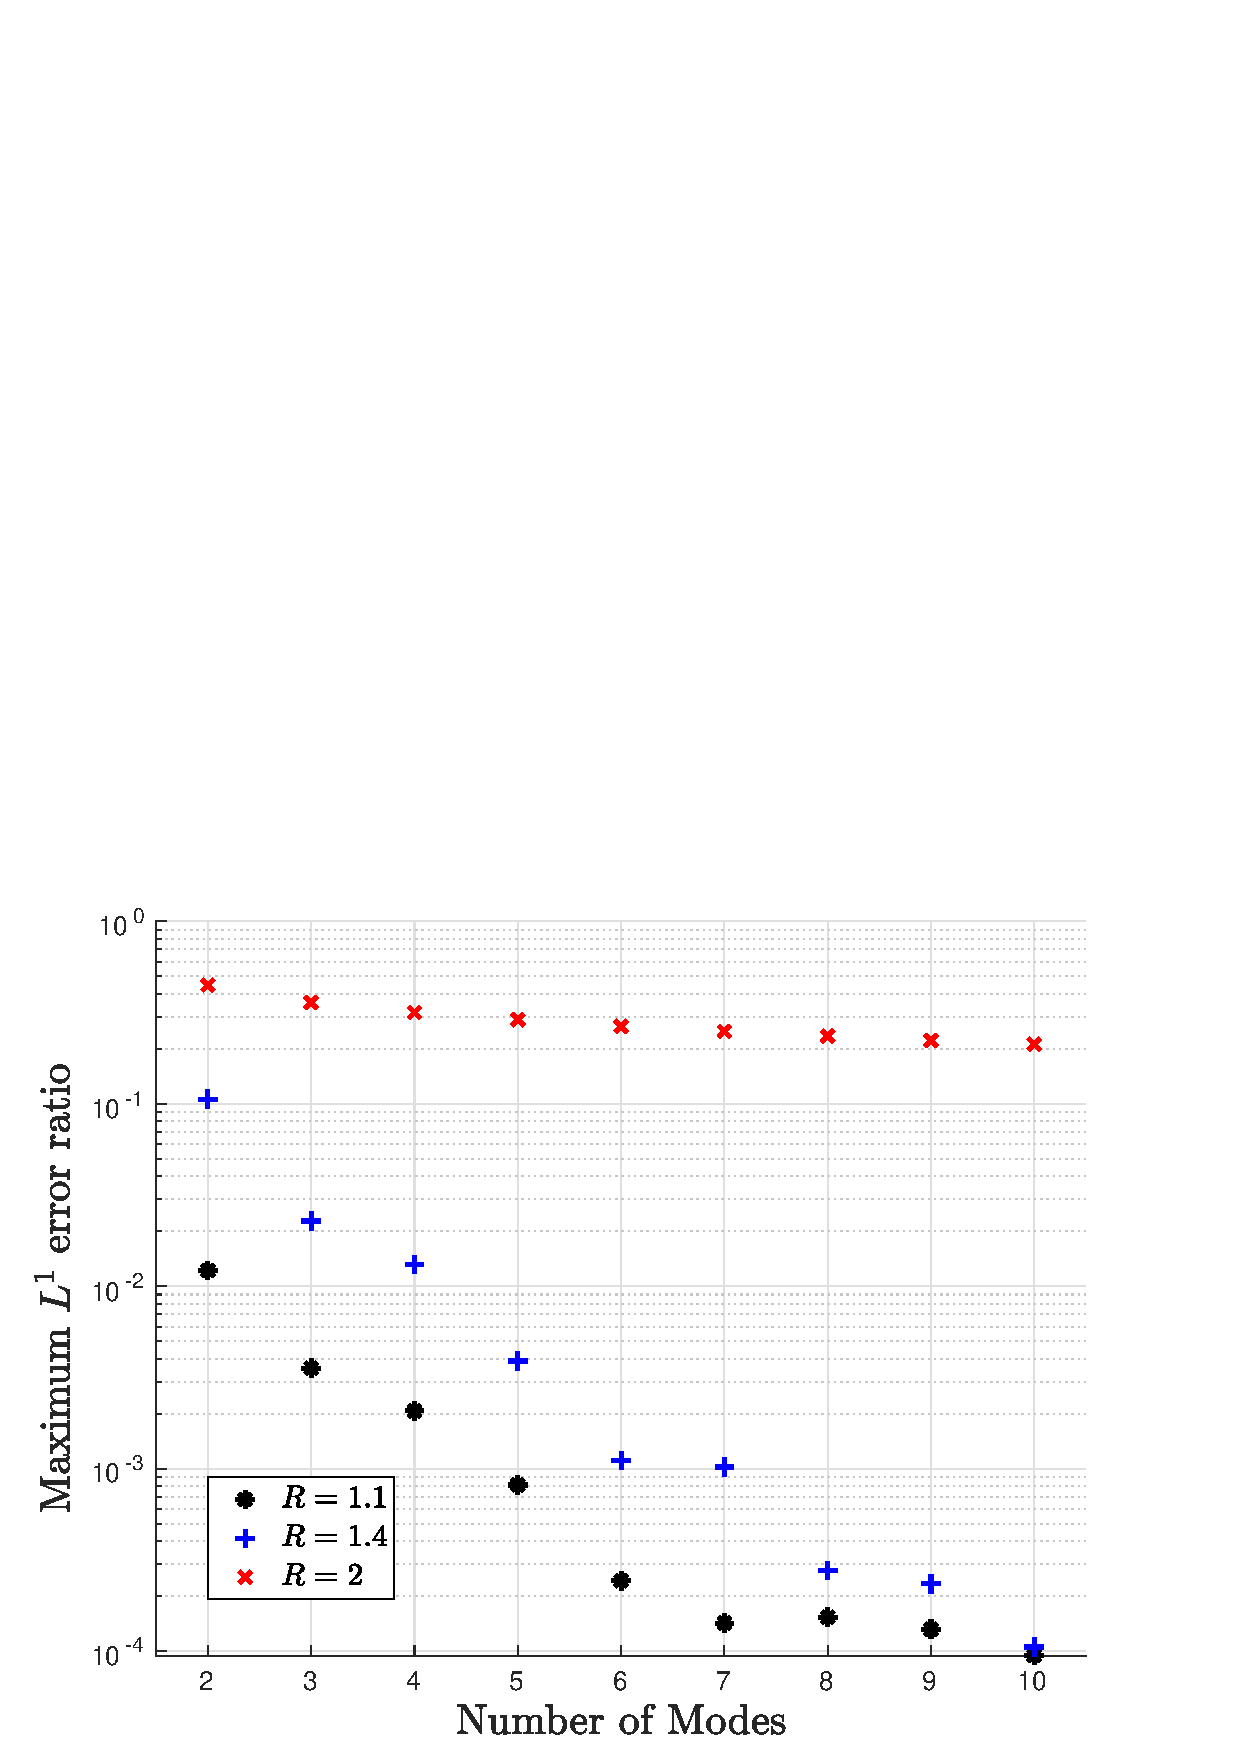
\includegraphics[width=0.8\linewidth]{06-appendix/SpectralMethodBoltzmann/Figures/free_stream_L1_err.pdf}}
\caption{Maximum ratio  of $L^1$ error between computed and exact solutions to $L^1$ norm of the exact solution. \radapt{Birrell:2014gea}.}\label{fig:freeStreamL1Err}
\end{figure}
%%%%%%%%%%%%%%%%%%%%%%%%%%%%%%%%%%%%%%%

To show that the numerical integration accurately captures the mode coefficients of the exact solution, \req{exactSol}, in Figure \ref{fig:freeStreambErr} we show the error between the computed coefficients and actual coefficients, denoted by $\tilde b_n$ and $b_n$ respectively,
\begin{equation}\label{modeErrDef}
\text{error}_n=\max_{t} |\tilde{b}_n(t)-b_n(t)|\,,
\end{equation}
 where the evolution of the system was computed using $N=10$ modes.



In Figure  \ref{fig:freeStreamL1Err} we show the error between the exact solution $f$, and the numerical solution $f^N$ computed using $N=2,...,10$ modes over the solution time interval, where we define the error by
\begin{equation}\label{fErr}
\text{error}_N=\max_{t} \frac{\int |f-f^N|dy}{\int |f|dy}\,.
\end{equation}
%%%%%%%%%%%%%%%%%%%%%%%%%%%%%%%%%%%%%%%
\begin{figure}[ht]
\centerline{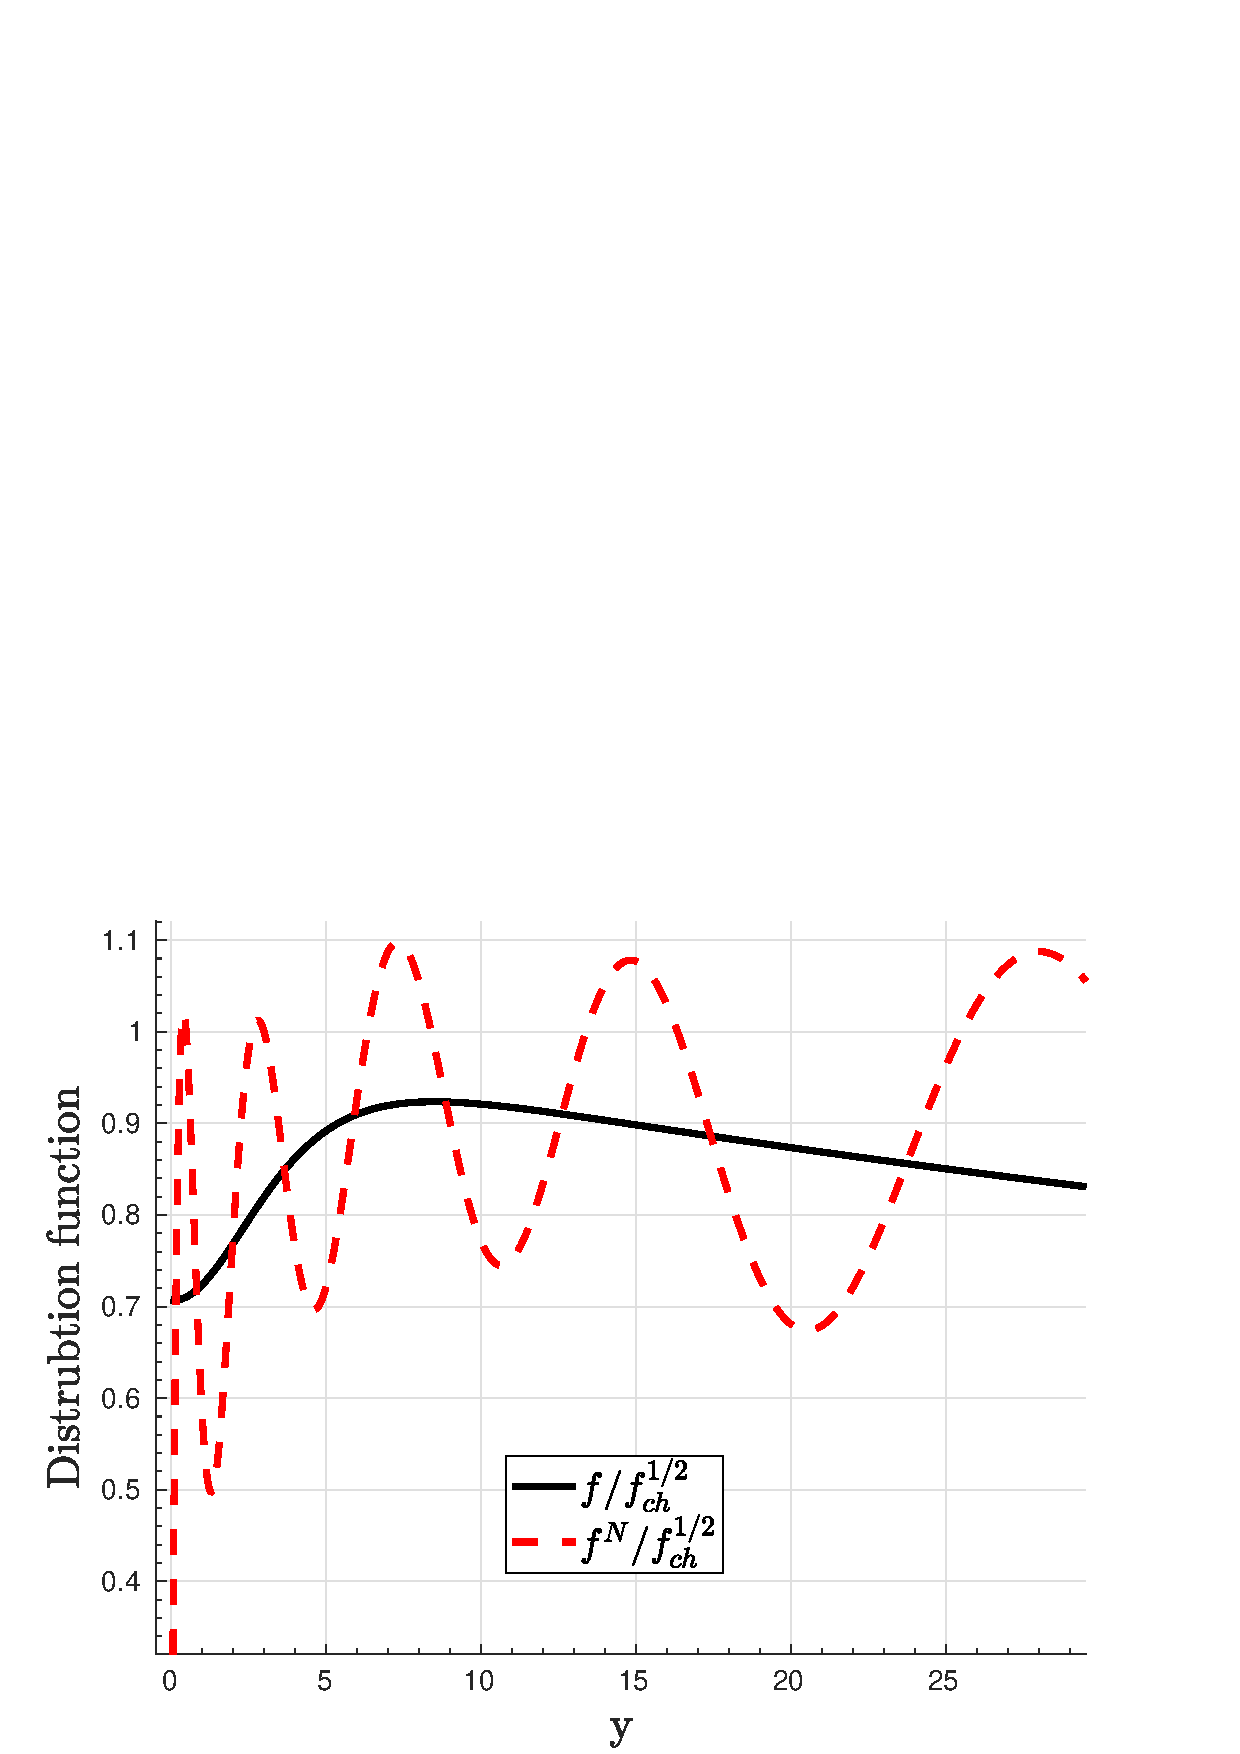
\includegraphics[width=0.8\linewidth]{06-appendix/SpectralMethodBoltzmann/Figures/free_stream_approx_T_r_2.pdf}}
\caption{Approximate and exact solution for a reheating ratio $R=2$ and $N=10$ modes. \radapt{Birrell:2014gea}.}\label{fig:freeStreamApproxTr2}
 \centerline{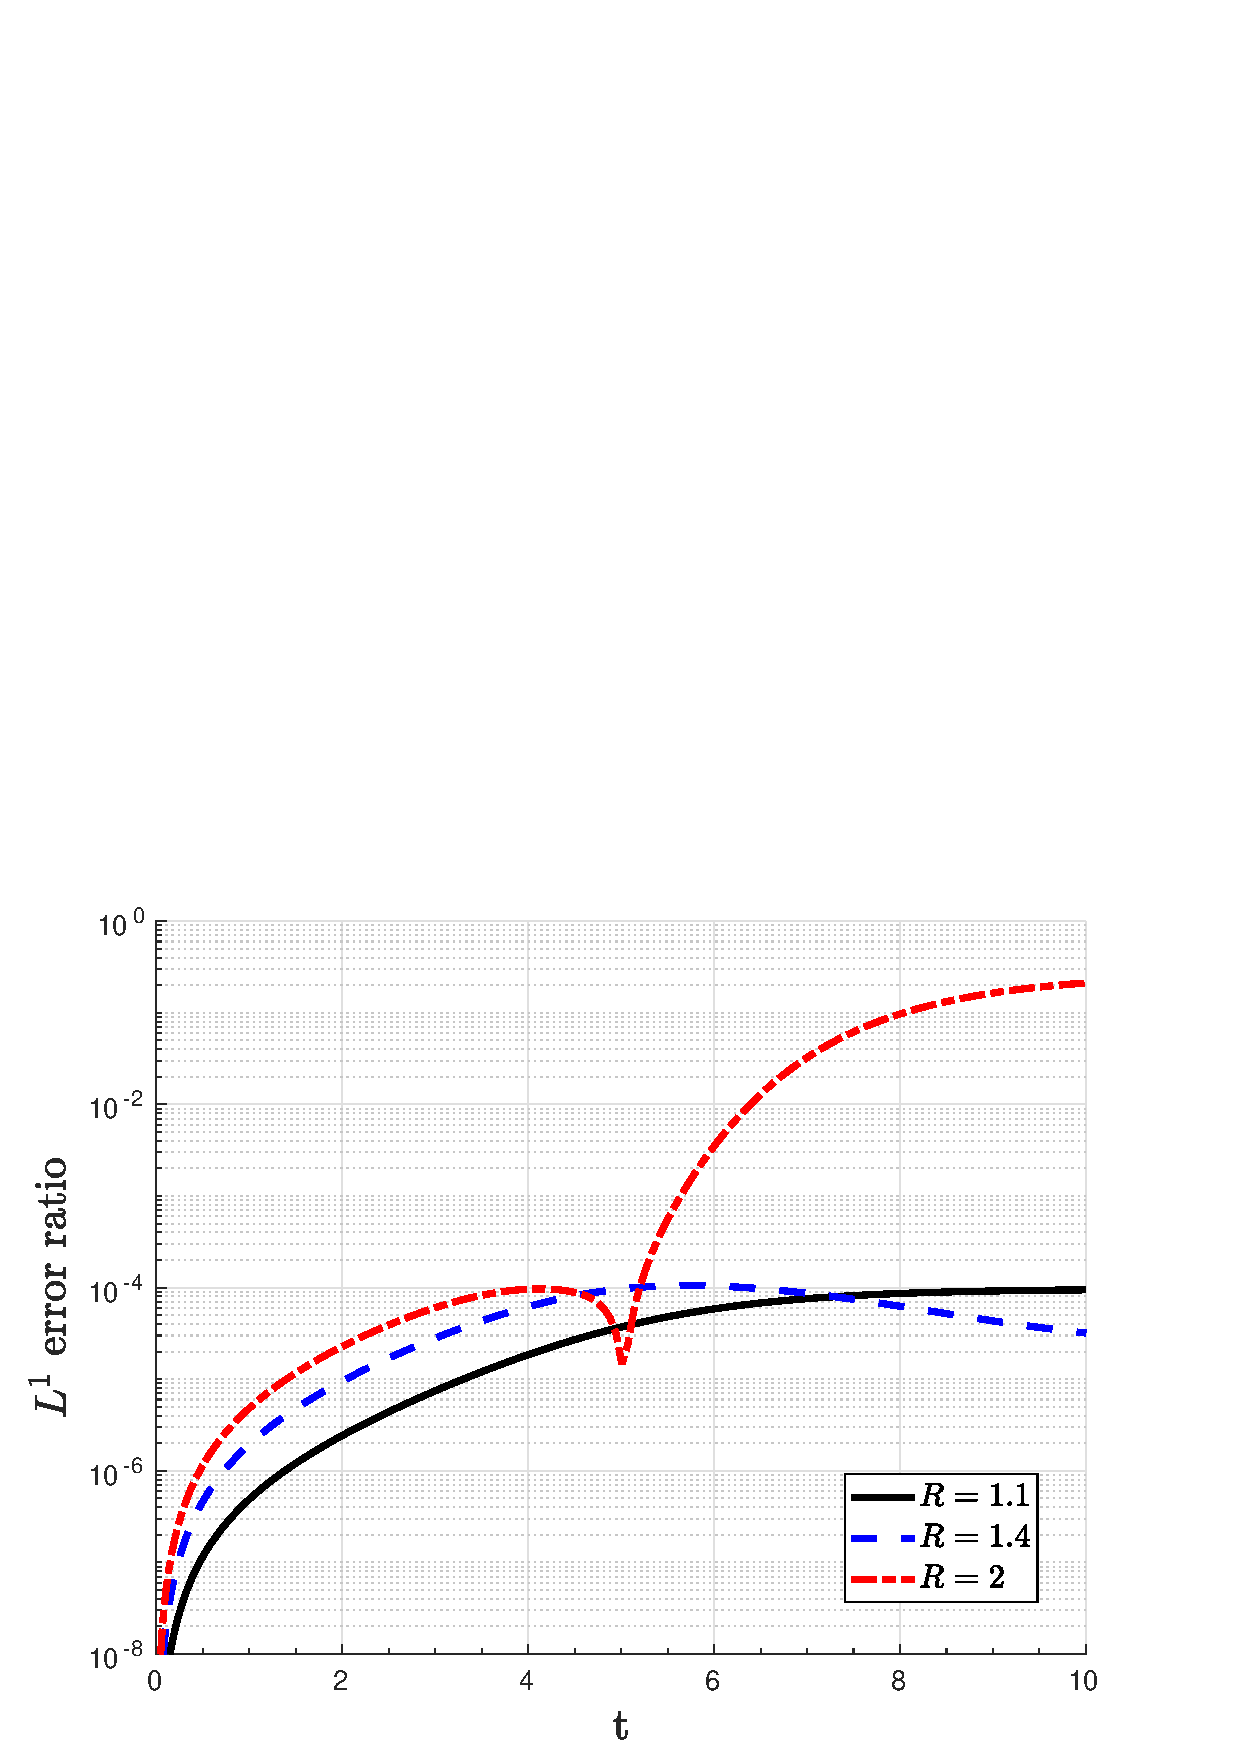
\includegraphics[width=0.8\linewidth]{06-appendix/SpectralMethodBoltzmann/Figures/free_stream_L1_err_time.pdf}}
\caption{$L^1$ error ratio as a function of time for $N=10$ modes. \radapt{Birrell:2014gea}.}\label{fig:freeStreamL1errTime}
\end{figure}
%%%%%%%%%%%%%%%%%%%%%%%%%%%%%%%%%%%%%%%
For $R=1$ and $R=1.4$  the chemical equilibrium method works reasonably well (as long as the number of modes is at least 4, so that the energy and number densities are properly captured) but for $R=2$ the approximate solution exhibits spurious oscillations, as seen in Figure \ref{fig:freeStreamApproxTr2}, and has significantly degraded $L^1$ error;  this behavior is expected based on the results in Section \ref{basisComparison}. Further clarifying the behavior, in Figure \ref{fig:freeStreamL1errTime}  we show the $L^1$ error ratio as a function of time for $N=10$ modes. In the $R=2$ case we see that the error increases as the reheating ratio approaches its asymptotic value of $R=2$ as $t\rightarrow\infty$.  As we will see, our methods achieves a much higher accuracy for a small number of terms in the case of large reheating ratio due to the replacement of dilution temperature scaling with the dynamical effective temperature $T$.  


%%%%%%%%%%%%%%%%%%%%%%%%%%%%%%%%%%%%%%%%%%%%%%%%%%%%%%
\noindent{\bf Chemical Non-Equilibrium Method:}\\
We now solve  \req{freeStreamToy} using the chemical nonequilibrium method, with the orthonormal basis defined by the weight function \req{weight} for $N=2,...,10$ modes, a prescribed numerical integration tolerance of $10^{-13}$, and asymptotic reheating ratios of $R=1.1$, $R=1.4$, and $R=2$.  Recall that we are referring to $T$ and $\Upsilon$ as the first two modes ($n=0$ and $n=1$). 
%%%%%%%%%%%%%%%%%%%%%%%%%%%%%%%%%%%%%%%
\begin{figure}[ht]
\centerline{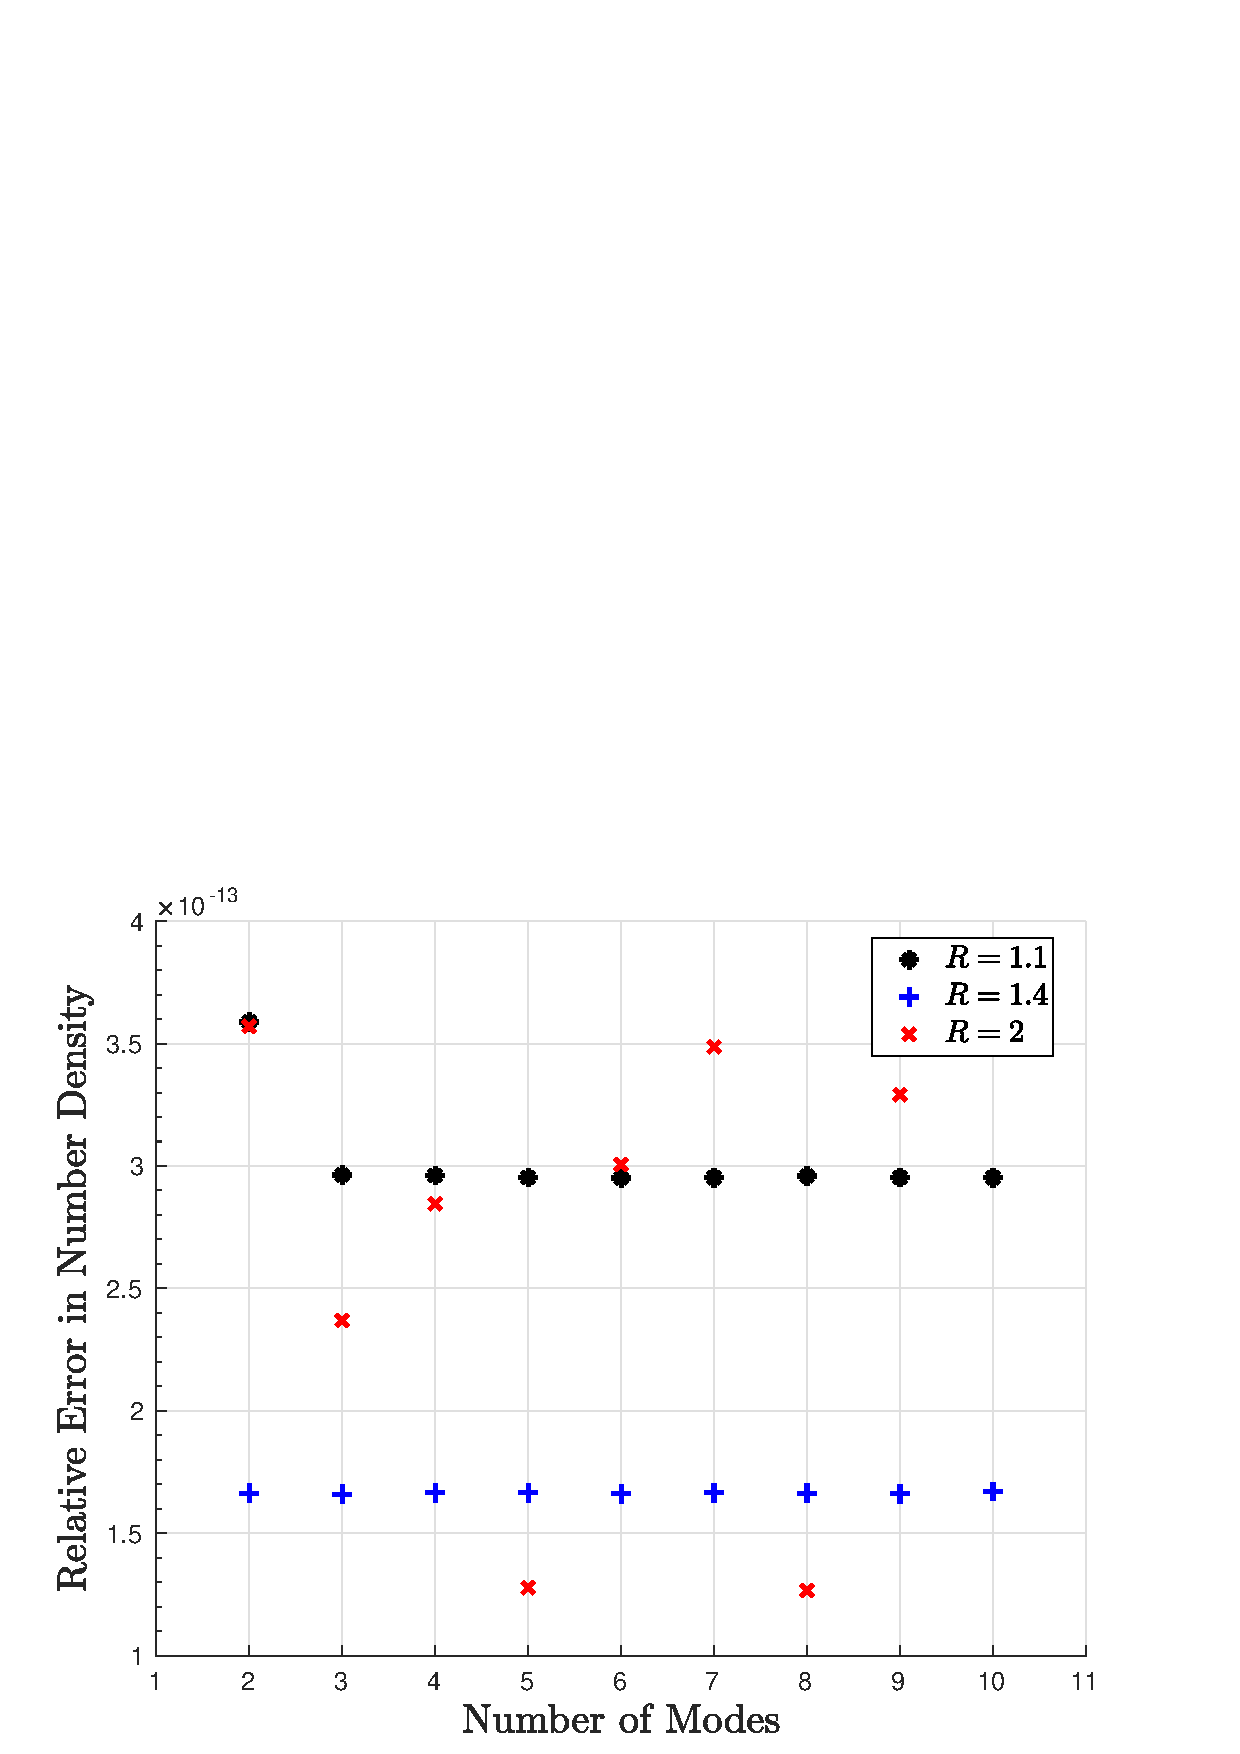
\includegraphics[width=0.9\linewidth]{06-appendix/SpectralMethodBoltzmann/Figures/keq_num_err.pdf}}
\caption{Maximum relative error in particle number density. \radapt{Birrell:2014gea}.}\label{fig:keqNumErr}
 \centerline{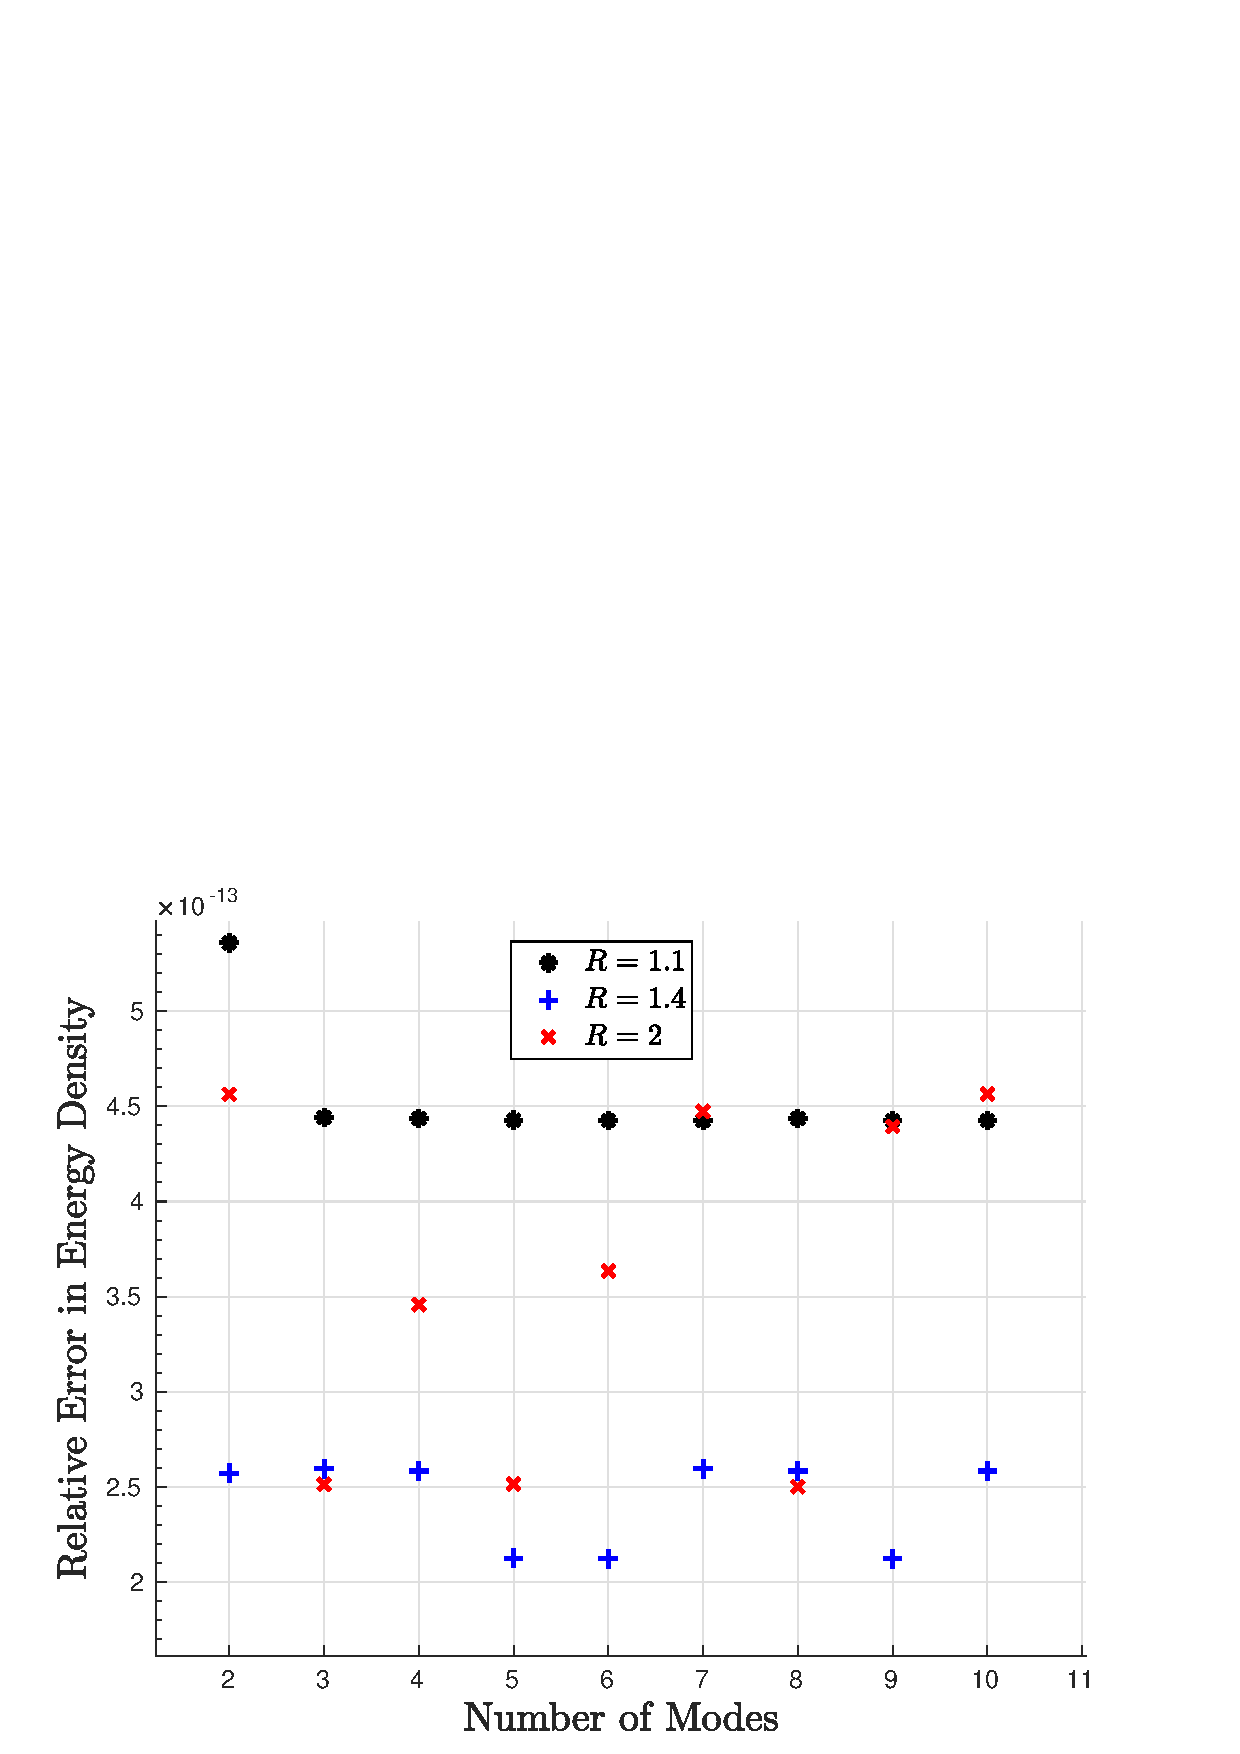
\includegraphics[width=0.9\linewidth]{06-appendix/SpectralMethodBoltzmann/Figures/keq_E_err.pdf}}
\caption{Maximum relative error in energy density. \radapt{Birrell:2014gea}.}\label{fig:keqEerr}
\end{figure}
%%%%%%%%%%%%%%%%%%%%%%%%%%%%%%%%%%%%%%%
In Figures \ref{fig:keqNumErr} and  \ref{fig:keqEerr} we show the maximum relative error over the time interval $[0,10]$ in the number densities and energy densities respectively for various numbers of computed modes. Even for only $2$ modes, the number and energy densities are accurate up to the integration tolerance level.  This is in agreement with the analytical expressions in \req{thEqMoments}.



%%%%%%%%%%%%%%%%%%%%%%%%%%%%%%%%%%%%%%%
\begin{figure}[ht]
\centerline{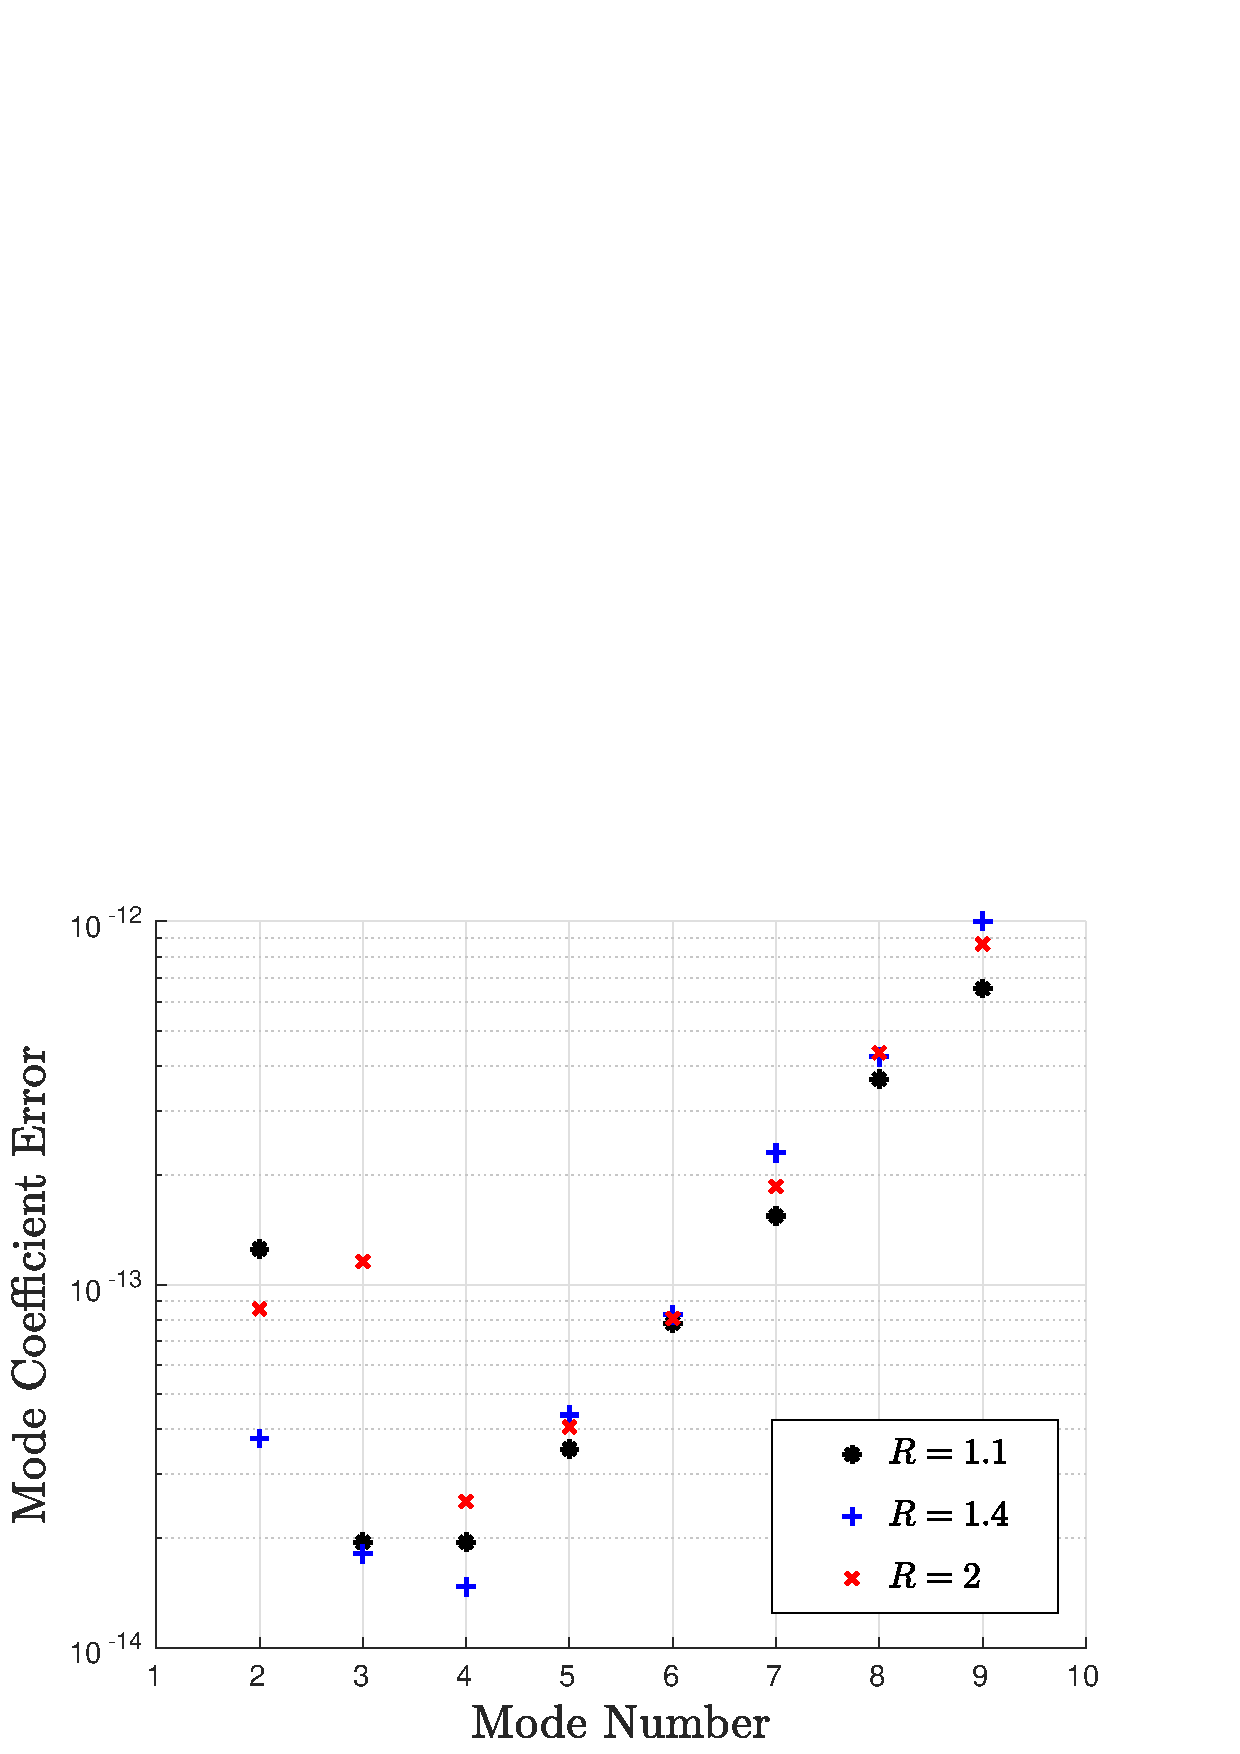
\includegraphics[width=0.9\linewidth]{06-appendix/SpectralMethodBoltzmann/Figures/keq_b_err.pdf}}
\caption{Maximum error in mode coefficients. \radapt{Birrell:2014gea}.}\label{fig:keqbErr}
\centerline{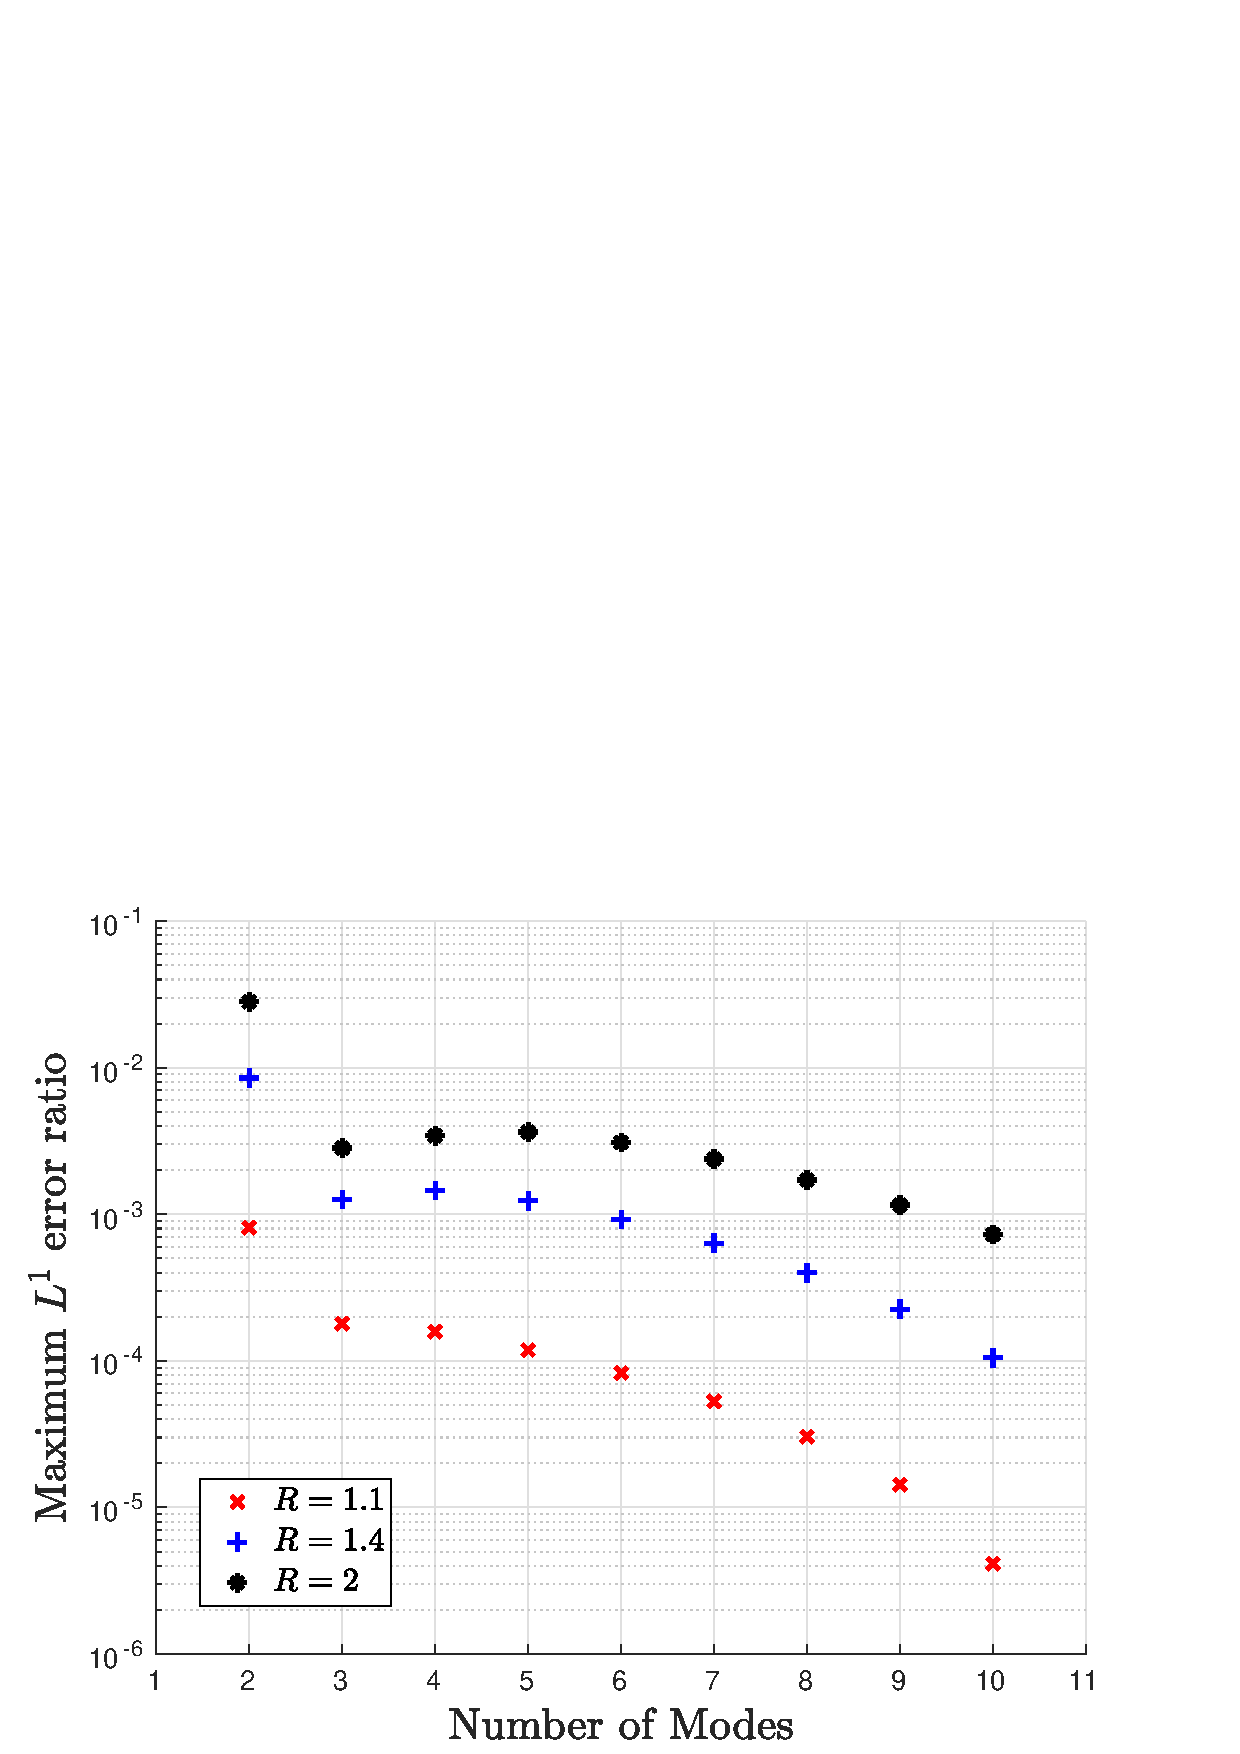
\includegraphics[width=0.9\linewidth]{06-appendix/SpectralMethodBoltzmann/Figures/keq_L1_err.pdf}}
\caption{Maximum ratio of $L^1$ error between computed and exact solutions to $L^1$ norm of the exact solution. \radapt{Birrell:2014gea}.}\label{fig:keqL1Err}
\end{figure}
%%%%%%%%%%%%%%%%%%%%%%%%%%%%%%%%%%%%%%%


To show that the numerical integration accurately captures the mode coefficients of the exact solution, \req{exactSol}, in Figure \ref{fig:keqbErr} we show the error in the computed mode coefficients \req{modeErrDef}, where the evolution of the system was computed using $N=10$ modes. In Figure \ref{fig:keqL1Err} we show the error between the approximate and exact solutions, computed as in \req{fErr} for $N=2,...,10$ and $R=1.1$, $R=1.4$, and $R=2$ respectively.  For most mode numbers and $R$ values, the error using $2$ modes is substantially less than the error from the chemical equilibrium\index{chemical equilibrium} method using $4$ modes.  The result is most dramatic for the case of large reheating, $R=2$, where the spurious oscillations from the chemical equilibrium solution are absent in our method, as seen in Figure \ref{fig:keqApproxTr2}, as compared to the chemical equilibrium method in Figure \ref{fig:freeStreamApproxTr2}.  Note that we plot from $z\in [0,15]$ in comparison to $y\in[0,30]$ in Figure \ref{fig:keqApproxTr2} due to the relation $z=y/R$ as discussed in Section \ref{basisComparison}. Additionally, the error no longer increases as $t\rightarrow\infty$, as it did for the chemical equilibrium method, see Figure \ref{fig:keqL1errTime}.  In fact it decreases since the exact solution approaches chemical equilibrium at a reheated temperature and hence can be better approximated by $f_\Upsilon$. 

In summary, in addition to the reduction in the computational cost when going from $4$ to $2$ modes, we also reduce the error compared to the chemical equilibrium method, all while accurately capturing the number and energy densities. 

%%%%%%%%%%%%%%%%%%%%%%%%%%%%%%%%%%%%%%%
\begin{figure}[ht]
\centerline{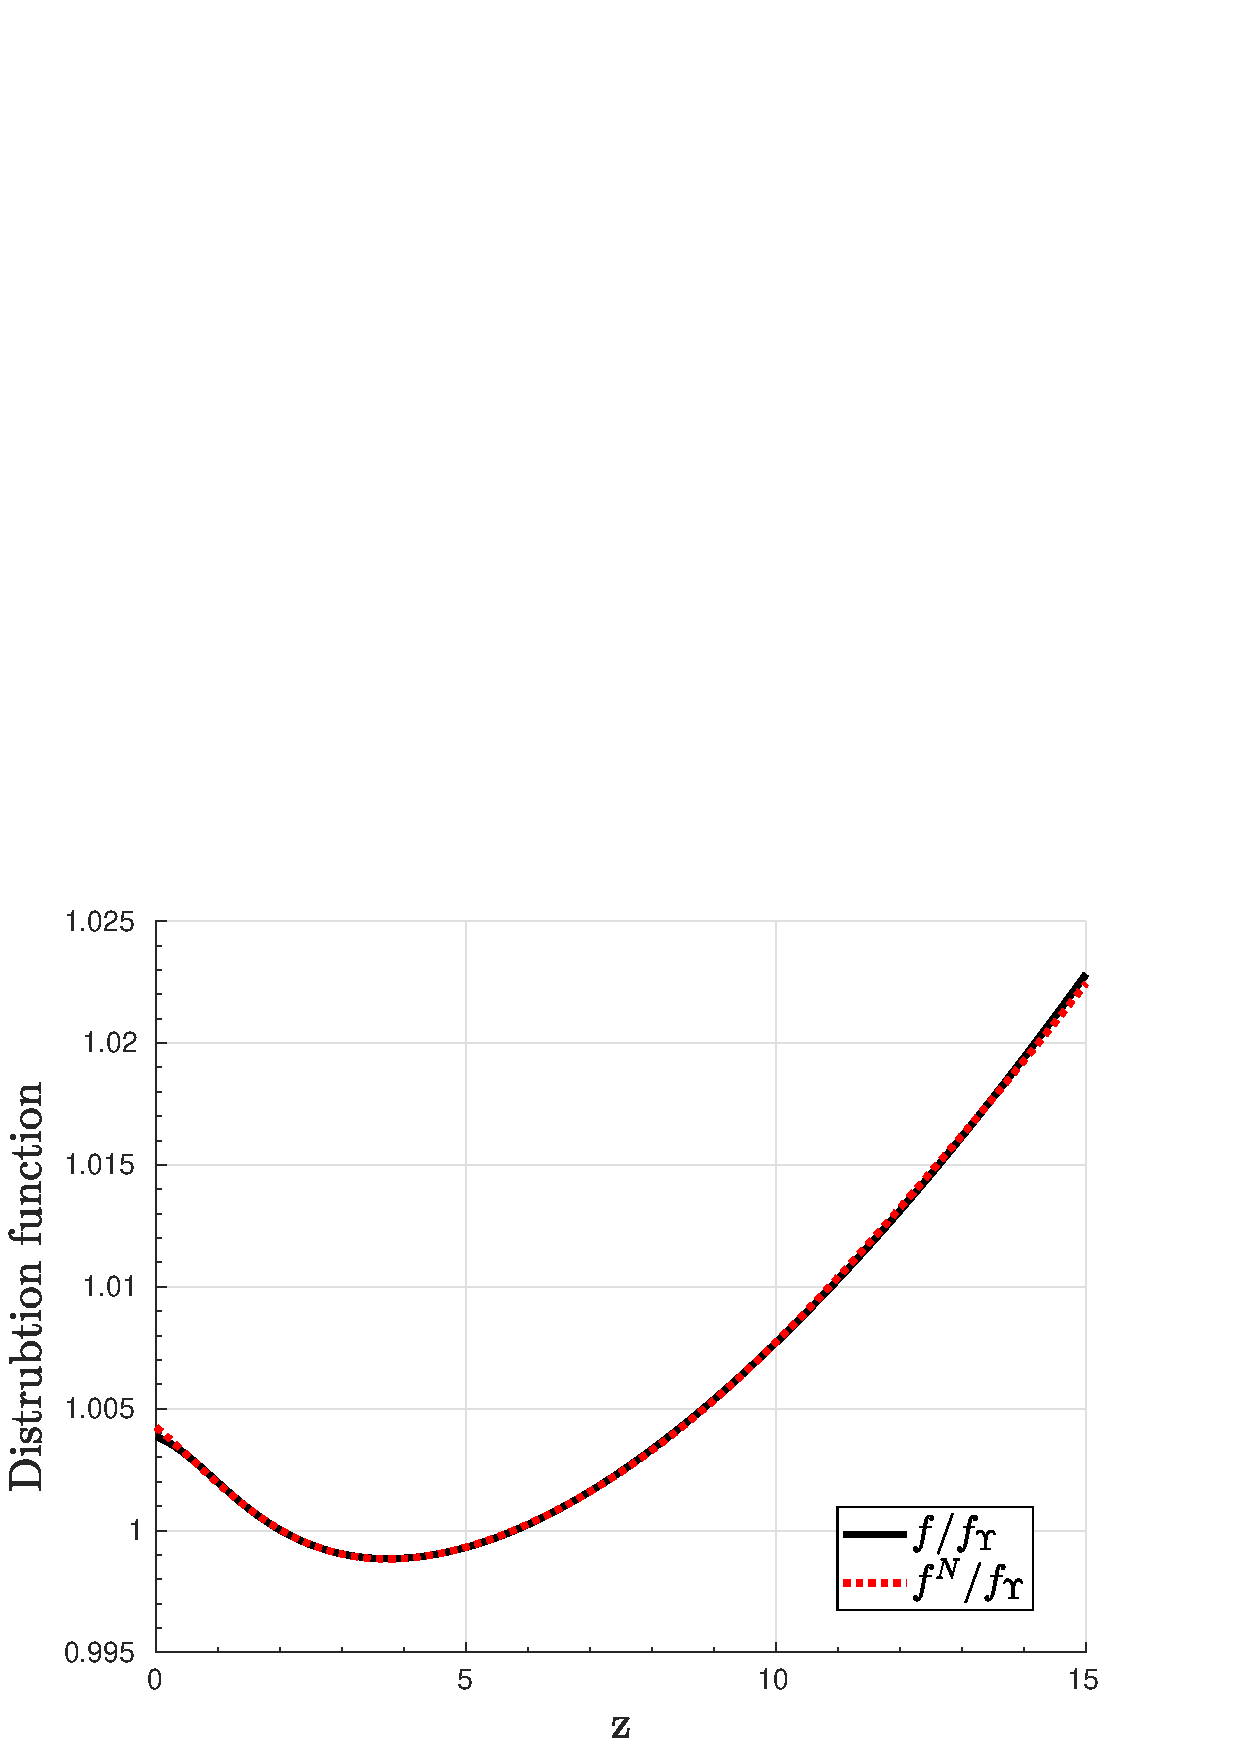
\includegraphics[width=0.9\linewidth]{06-appendix/SpectralMethodBoltzmann/Figures/keq_approx_T_r_2.pdf}}
\caption{Approximate and exact solution for $R=2$ obtained with two modes. \radapt{Birrell:2014gea}.}\label{fig:keqApproxTr2}
\centerline{\includegraphics[width=0.9\linewidth]{06-appendix/SpectralMethodBoltzmann/Figures/keq_L1_err_time.pdf}}
\caption{$L^1$ error ratio as a function of time for $n=10$ modes. \radapt{Birrell:2014gea}.}\label{fig:keqL1errTime}
\end{figure}
%%%%%%%%%%%%%%%%%%%%%%%%%%%%%%%%%%%%%%%


\clearpage
\input{16NeutrinoScatteringIntegrals.tex}

%%%%%%%%%%%%%%%%%%%%%%%%
\addcontentsline{toc}{section}{List of Figures}
\listoffigures
%%%%%%%%%%%%%%%%%%%%%%%%

%%%%%%%%%%%%%%%%%%%%%%%%
\addcontentsline{toc}{section}{References}
%\bibliographystyle{sn-aps}
\bibliographystyle{sn-basic}
\bibliography{refs.bib}

%%%%%%%%%%%%%%%%%%%%%%%%
\addcontentsline{toc}{section}{Index}
\printindex
%%%%%%%%%%%%%%%%%%%%%%%%
\end{document}
